%!TEX TS-program = xelatex
%!TEX encoding = UTF-8 Unicode

\documentclass{Dissertate}

\usepackage{graphicx} 
\usepackage{amsmath}
\usepackage{hyperref}
\usepackage{amsfonts}
%\usepackage{amsmath}
\usepackage{amssymb}
\usepackage{amsthm}
\usepackage{subeqnarray}
\usepackage{epstopdf}
\usepackage{natbib}
%\usepackage{deluxetable}
%\bibliographystyle{apj}

\newcommand{\emgr}[1]{\emph{ \color{gray} #1}}

\newcommand{\ie}{i.e.\ }
\newcommand{\eg}{e.g.\ }
\newcommand{\p}{\partial}
\newcommand{\xv}{\vc{x}}
\newcommand{\kv}{\vc{k}}
\newcommand{\brak}[1]{\langle #1\rangle}


\newcommand{\gcc}{\;\mathrm{g\; cm^{-3}}}
\newcommand{\gsc}{\;\mathrm{g\; cm^{-2}}}
\newcommand{\cm}{\; {\rm cm}}
\newcommand{\mm}{\; {\rm mm}}
%\newcommand{\ps}{\; {\rm s^{-1}}}
\newcommand{\km}{\; {\rm km}}

\newcommand{\AU}{\; {\rm AU}}
\newcommand{\yr}{\; {\rm yr}}
\def\K{\; {\rm K}}

\newcommand{\vcs}[1]{\mbox{\boldmath{$\scriptstyle{#1}$}}}
\newcommand{\vc}[1]{\mbox{\boldmath{$#1$}}}
\newcommand{\nab}{\vc{\nabla}}
\DeclareMathSymbol{\varOmega}{\mathord}{letters}{"0A}
\DeclareMathSymbol{\varSigma}{\mathord}{letters}{"06}
\DeclareMathSymbol{\varPsi}{\mathord}{letters}{"09}

\newcommand{\eq}[1]{equation\,(\ref{#1})}
\newcommand{\Eq}[1]{Equation\,(\ref{#1})}
\newcommand{\Eqs}[2]{Equations (\ref{#1}) and~(\ref{#2})}
\newcommand{\Eqss}[2]{Equations (\ref{#1})--(\ref{#2})}
\newcommand{\Eqsss}[3]{Equations (\ref{#1}), (\ref{#2}) and~(\ref{#3})}
\newcommand{\App}[1]{Appendix~\ref{#1}}
\newcommand{\Sec}[1]{Sect.~\ref{#1}}
\newcommand{\Chap}[1]{Chapter~\ref{#1}}
\newcommand{\Fig}[1]{Figure~\ref{#1}}
\newcommand{\Figs}[2]{Figs.~\ref{#1} and \ref{#2}}
\newcommand{\Figss}[2]{Figs.~\ref{#1}--\ref{#2}} 
\newcommand{\Tab}[1]{Table \ref{#1}}

\newenvironment{packed_item}{
\begin{itemize}
  \setlength{\itemsep}{1pt}
  \setlength{\parskip}{0pt}
  \setlength{\parsep}{0pt}
}{\end{itemize}}

\newcommand{\delad}{\nabla_{\rm ad}}
\newcommand{\delrad}{\nabla_{\rm rad}}
\newcommand{\Rg}{\mathcal{R}}
\newcommand{\RB}{R_{\rm B}}
\newcommand{\RH}{R_{\rm H}}
\newcommand{\co}{_{\rm c}}
\newcommand{\pla}{_{\rm p}}
\newcommand{\di}{_{\rm d}}
\newcommand{\cb}{_{\rm RCB}}
\newcommand{\mc}{m_{\rm c \oplus}}
\newcommand{\mcn}[1] { m_{ \rm c #1} }
\newcommand{\mpn}[1] { m_{ \rm p #1} }
\newcommand{\MC}{M_{\rm crit}}
\newcommand{\au}{a_\oplus}
\newcommand{\aun}[1]{ a_{#1} }
\def\crit{_{\rm{c, crit}}}



\begin{document}

% the front matter
% Some details about the dissertation.
\title{Origins of Gas Giant Compositions: The Role of Disk Location and Dynamics}
\author{Ana-Maria A. Piso}
\advisor{Karin I. \"Oberg}

% ... about the degree.
\degree{Doctor of Philosophy}
\field{Astronomy and Astrophysics}
\degreeyear{2016}
\degreemonth{May}
\department{Astronomy}

% ... about the candidate's previous degrees.
\pdOneName{B.S.}
\pdOneSchool{Boston University}
\pdOneYear{2018}

\pdTwoName{M.A.}
\pdTwoSchool{Monster's Univeristy}
\pdTwoYear{2021}

\maketitle
\copyrightpage

\setstretch{1.2}
\abstractpage
\tableofcontents
%\authorlist
\listoffigures
\dedicationpage
\acknowledgments

\doublespacing

% include each chapter...
%\setcounter{chapter}{-1}  % start chapter numbering at 0
\chapter{Introduction}

In recent years, the field of giant planet formation has aimed to answer two fundamental questions:

\begin{enumerate}
\item Where in the protoplanetary disk can gas giants form?
\item What compositions will the formed giant planets have obtained?
\end{enumerate} 

We can start uncovering the answers to these questions through a combination of studying planet formation in protoplanetary disks, the end-results of planet formation (i.e., exoplanets), and the architecture and composition of our own Solar System. In the last two decades, more than one thousand extrasolar planets (exoplanets)
have been discovered \citep{batalha14}. Their diversity in terms of mass, radius, location and composition
\citep{lissauer14} provides an exciting field of research, with the eventual goal of finding planets that are
similar to our own Earth and may sustain life. For this purpose, it is thus crucial to explore
and understand how planets obtain their compositions. Observations of Earth-like planets
that can provide useful insight about their composition are challenging --- the solid interior
structure of terrestrial planets cannot be detected, and their gaseous envelopes are small by
comparison (both in mass and radius), which makes it difficult to obtain atmospheric spectra
and find out what chemical compounds they are made of. 

To obtain constraints on how planets obtain their compositions, we instead turn to giant planets. Gas giants contain most
of their mass in their atmosphere, hence their chemical composition is largely determined by that
of their envelopes. These envelopes are observable with existing telescopes. The last few years have seen a substantial increase in the number of
giant planets with observed atmospheric spectra (e.g., \citealt{debes13}, \citealt{kreidberg15}), which has enhanced our
understanding of these planets' chemical structure, and has provided us with quantitative
information about the abundances of various compounds in their envelopes besides hydrogen
and helium. Gas giant formation is also important to constrain since gas giants shape the architecture of planetary systems and affect the
delivery of volatile compounds to terrestrial planets, which has direct consequences for the
habitability of worlds similar to our own. Thus testing theories of planet formation against
gas giant compositions will help constrain planet formation theories more generally.


Both terrestrial and giant planets are born in protoplanetary disks, which implies that
their compositions are determined by and tightly linked to the structure and
composition of the disk. The chemical and dynamical evolution of disks, as well the
formation of giant planets have both been previously investigated in isolation. However, the
coupled chemo-dynamical disk evolution, planet compositions, and most importantly the
disk-planet connection have not yet been considered in detail. In this thesis, we uncover some of the answers to this issue from two standpoints: (1) by looking at the role of disk location in setting the conditions for the formation of wide-separation gas giants, and (2) by investigating how the structure and chemical composition of the protoplanetary disk at different radii affects the composition of nascent giant planets.


\section{The Core Accretion Mechanism and Its Challenges}

Gas giants are widely believed to form through core accretion (e.g., \citealt{pollack96}), a theory in which
solid protoplanetary cores grow large enough to accumulate a massive atmosphere. In this
model, planetesimals in a disk grow larger through collisions, eventually forming a planetary
embryo, which continues to grow by attracting planetesimals in its neighborhood. Once an
embryo becomes large enough so that its escape velocity exceeds the thermal velocity of the
nebular gas in its vicinity, it starts accumulating a gaseous envelope. From this point on, the
accretion of gas is regulated by the pressure support within the envelope --- the amount of
gas a core can accumulate is limited by the atmosphere's ability to radiate away the energy
due to the incoming planetesimals, as well as by envelope contraction.

Protoplanetary disks dissipate on relatively short timescales of a few Myr \citep{williams11}. This implies that cores must grow fast in order to become large enough to attract massive atmospheres, and thus they need high planetesimal accretion rates. Studies that consider such high and constant rates (e.g., \citealt{stevenson82}, \citealt{boden86}, \citealt{wuchterl93}, \citealt{rafikov06}) find that the envelope accumulating around the planet is in steady state at all times, since all the energy due to the incoming planetesimals is radiated away by the atmosphere. It follows that the core and envelope grow simultaneously, and the mass of the atmosphere is a function of the core mass. Once the core and atmosphere have attained comparable masses, a rapid phase of runaway gas accretion starts and the gas giant can form. In this steady state scenario, there is therefore a uniquely determined core mass at which runaway accretion commences, called the critical core mass $M_{\rm crit}$. High planetesimal accretion rates cause the core to grow quickly, but this poses an additional challenge: fast accretion heats up the core's atmosphere, increases pressure support and inhibits the ability of the envelope to cool and contract, thus eventually increasing $M_{\rm crit}$. This is particularly challenging in the outer disk, where long dynamical times prevent large cores from forming before disk dissipation. \citet{rafikov11} shows that core accretion cannot operate beyond 40-50 AU at the accretion rates required to form the core and the atmosphere on the same timescale. 

%\begin{figure}[t!]
%\centering
%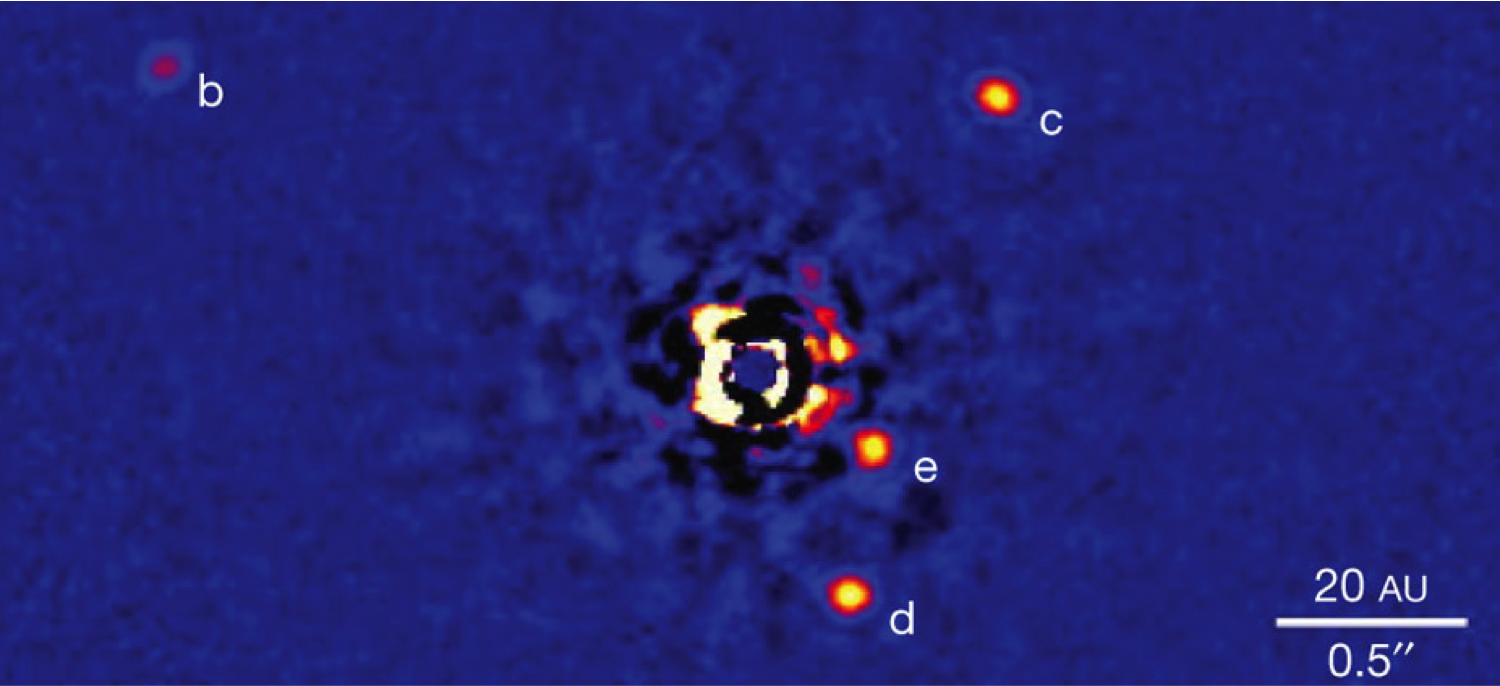
\includegraphics[width=0.8\textwidth]{figures/HR8799.png}
%%\vspace{-0.5in}
%\caption{The directly imaged HR 8799 system. Planets are located at 14.5 AU, 24 AU, 38 AU and 68 AU. From \citet{marois10}. }
%\label{fig:HR8799}
%\end{figure}

All this seems to indicate that core accretion cannot work in the outer disk. This poses an intriguing question: could wide-separation gas giants, such as the HR 8799 system, have formed through core accretion? We can start answering this question by noting that planetesimal accretion does not need to be constant with time at a given location in the disk, which has been shown to be a viable scenario (e.g., \citealt{ikoma00}, \citealt{pollack96}). Figure 1 from \citet{pollack96} shows an example of this scenario. At early times, the core is in a high planetesimal accretion rate regime and grows fast, but the atmosphere remains small in comparison. As the planet depletes its feeding zone of solids, planetesimal accretion is reduced. From this point on, the core no longer grows significantly, and thus the energy due to planetesimals can no longer balance radiative losses by the atmosphere; now the envelope accumulates gas while undergoing Kelvin-Helmholtz contraction, until its mass approximately exceeds the core mass and runaway gas accretion begins. Since now the envelope grows with time, there is no longer a uniquely determined $M_{\rm crit}$ --- in this scenario, the critical core mass is that of a core than can accrete an atmosphere with a mass equal to its own on a timescale equal to the disk lifetime. 

%\begin{figure}[t!]
%\centering
%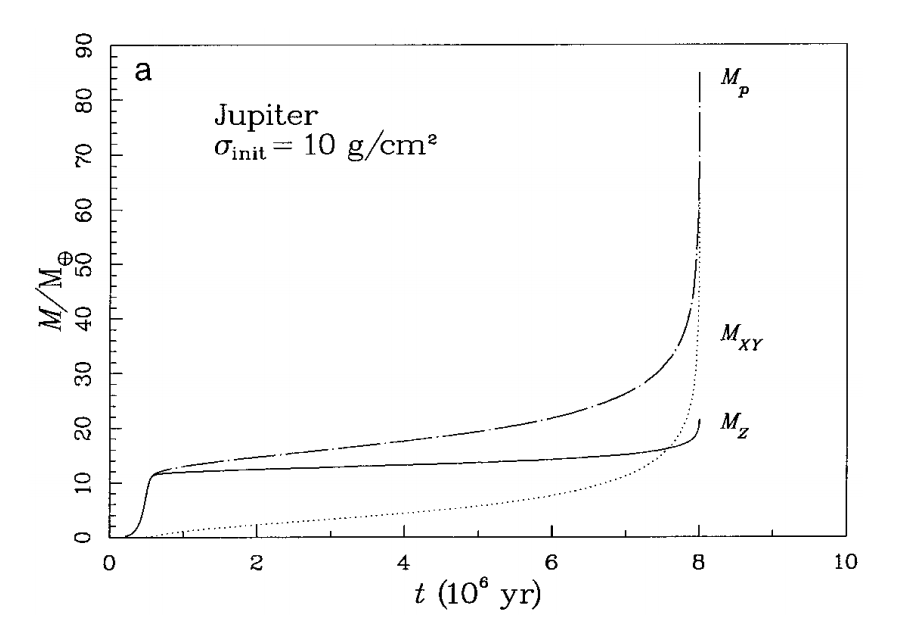
\includegraphics[width=0.8\textwidth]{figures/pollack.png}
%%\vspace{-0.5in}
%\caption{The evolution of a nascent planet's core (denoted with the subscript Z), atmosphere (denoted with the subscript XY), and total mass (denoted with the subscript p) as a function of time, for a planet forming at 5.2 AU through core accretion. The plot depicts the three phases of the planet's evolution: (1) core growth while atmosphere remains small (until $\sim1.2$ Myr), (2) atmospheric growth while core growth is practically stalled (until $\sim$7 Myr), and (3) runaway gas accretion.}
%\label{fig:pollack}
%\end{figure}

Such studies potentially provide a viable solution to the core accretion challenge at wide separations, but they are primarily focused on explaining the formation of Jupiter at 5.2 AU and thus do not explore a larger radii parameter space. Moreover, in order to truly understand whether core accretion can indeed work at stellocentric distances significantly larger than that of Jupiter, a more interesting question can be asked: what is the lowest possible core mass required to form a gas giant before disk dissipation? This minimum core mass is determined when planetesimal accretion has fully stopped, since additional accretion would actually increase this core mass (see above). Moreover, how does this minimum core mass depend on disk location, the properties of the nebular gas, and the opacity of the dust grains? We provide an answer to these questions in Chapters 2 and 3. 



\section{Dynamics and Chemistry in Protoplanetary Disks}

Protoplanetary disks are the result of the collapse of a molecular cloud. They are structures composed of gas and dust that are rotationally supported and that represent the birth environment of planets (Figure \ref{fig:proto}). Despite their simple geometry, disks are complex objects, whose structure and evolution are affected by a multitude of chemical and dynamical processes. The latter include transport of both dust through radial drift and gas through viscous gas accretion, as well as grain growth and dust settling to the disk midplane, which affect the disk structure. In terms of chemistry, the strongly irradiated disk surface is dominated by photochemical reactions, while the ionized lower layers have a rich ion-molecule chemistry. Finally, the cold disk midplane is mostly shielded from irradiation, and volatile compounds experience freeze-out.  Many of these processes are summarized in \citet{henning13}, and several of them are not yet fully understood.  Moreover, the timescales for various disk chemical and dynamical processes may be comparable at least in some parts of the disk \citep{semenov11}, which makes the coupling between chemistry and dynamics very challenging. 

Not all disk regions (and therefore all disk chemistry) are equally important to understand the disk-planet connection, however. Planets form in the midplane of disks, where the chemical structure is mainly set by condensation and sublimation of volatiles. As a first step we focus on the different dynamical and chemical processes that occur in the disk midplane, with the goal to understand their role and relative importance in shaping disk and planet compositions. 

\begin{figure}[h]
\centering
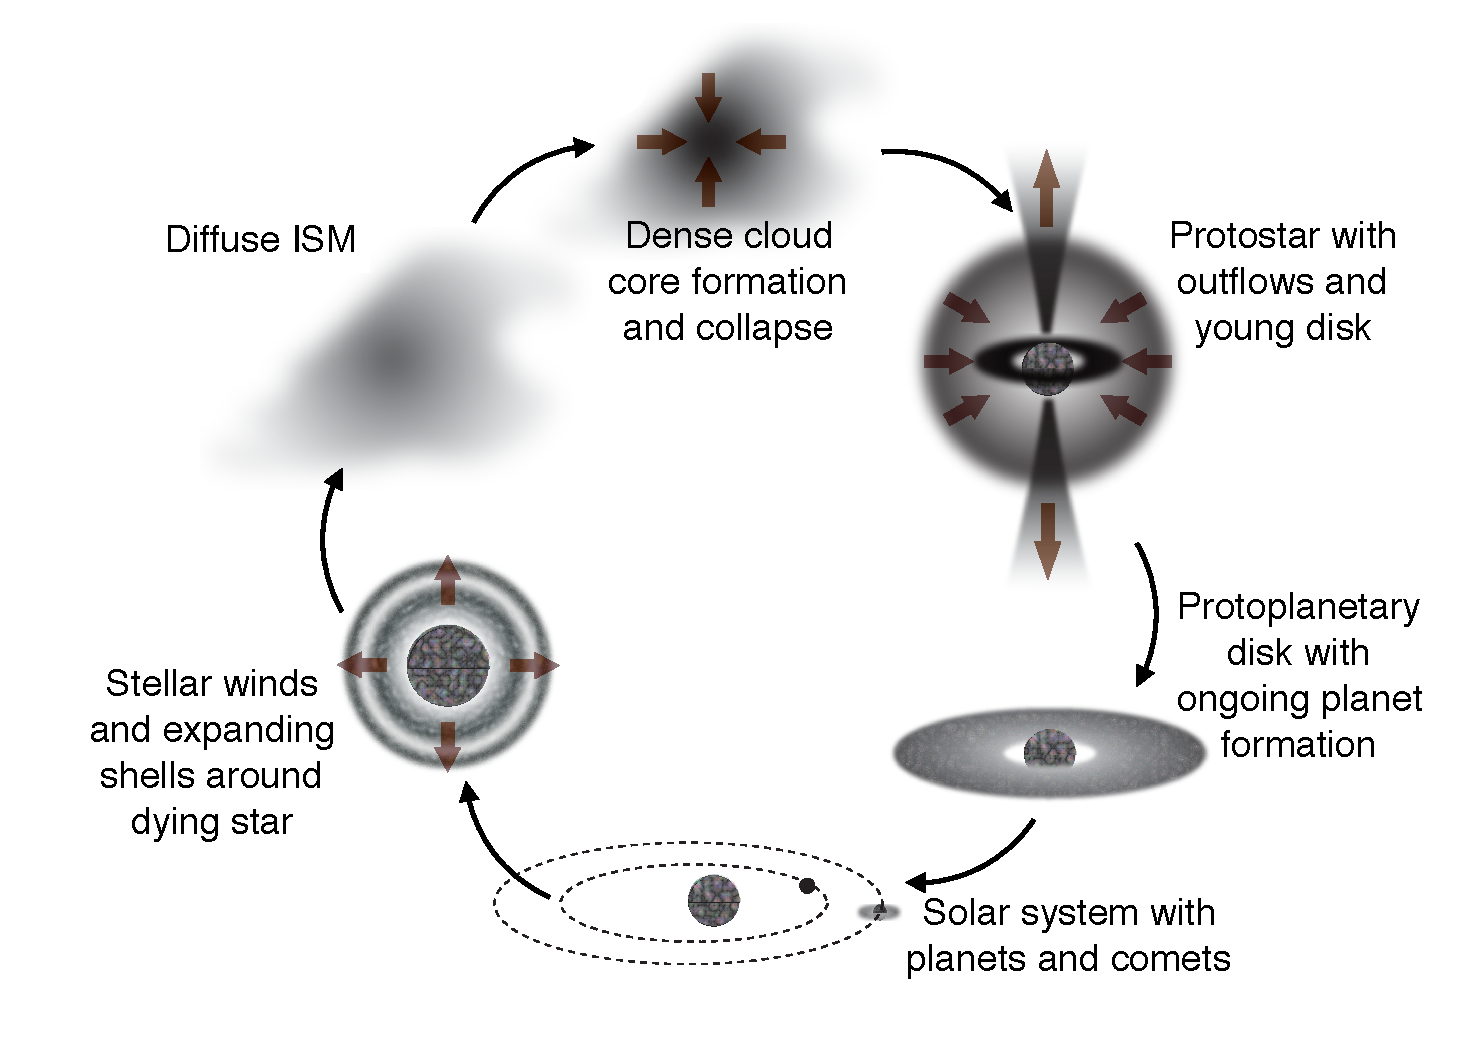
\includegraphics[width=0.8\textwidth]{figures/proto.pdf}
%\vspace{-0.5in}
\caption{The standard picture of molecular cloud to protostar to protoplanetary disk to planet formation. Reprinted with permission from \citet{oberg09}.}
\label{fig:proto}
\end{figure}

%\subsection{Disk Temperature and Density Structure}
\subsection{Disk Temperature and Density Structure}

The midplane temperature in a protoplanetary disk is set both by the irradiation from the host star and by accretion heating (e.g., \citealt{armitage10}). Accretion heating dominates in the inner disk (typically within a few AU) where the accretion flows are strongest, while the outer disk is dominated by stellar irradiation. While the irradiation component of the temperature simply follows a power-law in radius, the accretional component is determined by viscosity and the gas mass accretion rate, which in turn depend on the temperature itself, as well as the gas surface density (for a more complete review see \citealt{shakura73}). As the gas surface density changes with time in an active disk, it follows that determining the midplane temperature in an active disk in which both stellar irradiation and accretion heating contribute to the thermal evolution of the disk is non-trivial. We simplify this problem in Chapters 4 and 5 by assuming a steady-state disk with a constant mass accretion flow, and by solving the thin disk Shakura-Sunyaev equations.

The gas surface density in a viscous disk follows the continuity equation, and is set by both the disk temperature and viscosity. Infall of material onto the disk or outflow may also contribute to the gas surface density evolution \citep{birnstiel10}. The dust surface density can be described by an advection-diffusion equation (e.g., \citealt{birnstiel12}), where both the radial movement of the dust and diffusion contribute to its evolution. The diffusion term is due to the fact that the dust is turbulently mixed by the gas, which causes a change in the dust-to-gas ratio and thus a radial gradient in the ratio between solid and gas surface densities. In the case of small particles that are well coupled to the gas, the surface density follows that of the gas and a constant dust-to-gas ratio is maintained. The movement of larger particles, however, is affected both by radial drift, gas drag and diffusion, which cause the dust surface density to "decouple" from that of the gas. This results in depletion of solids in some disk regions and a pile-up in others, depending on a particle's radial drift velocity and the level of turbulent mixing. The dust surface density is further affected by grain growth and fragmentation. We do not address all these effects in Chapter 4 and 5, and instead assume a constant inflow of particles such that the dust surface density remains spatially and temporally constant. We note, however, that these effects have to be taken into account for a more realistic modeling of the dust surface density, and thus of the surface density evolution of volatiles, both in solid and gaseous form.  





%\begin{figure}[t!]
%\centering
%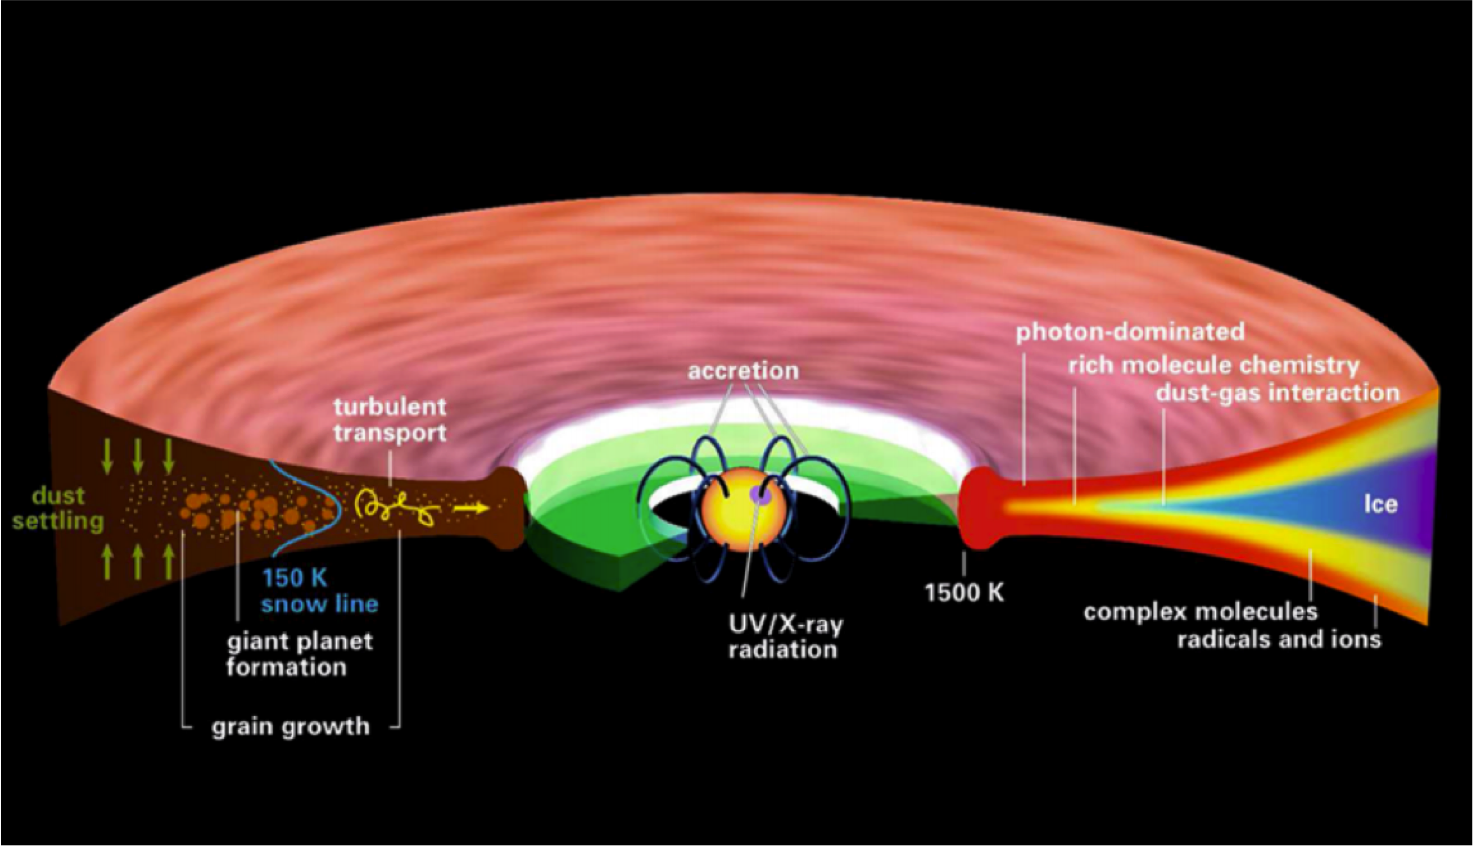
\includegraphics[width=0.8\textwidth]{figures/disk.png}
%%\vspace{-0.5in}
%\caption{Cross section through a protoplanetary disk showing various chemical and dynamical processes that occur in disks. From \citet{henning13}.}
%\label{fig:disk_henning}
%\end{figure}

%\begin{figure*}[t!]
%\centering
%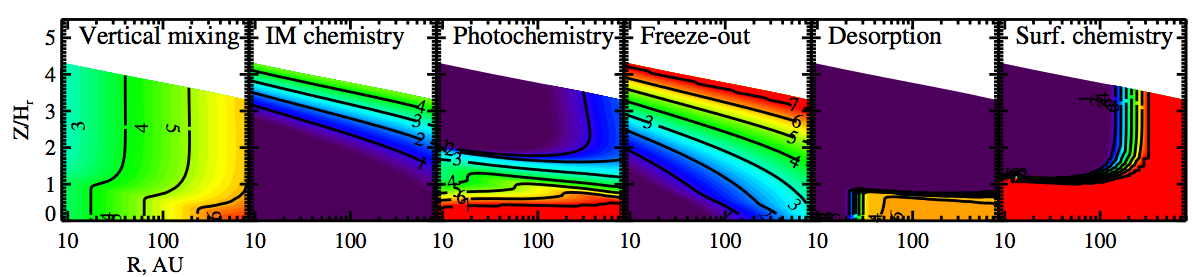
\includegraphics[width=0.8\textwidth]{figures/chemical_timescales.png}
%%\vspace{-0.5in}
%\caption{The distribution of characteristic chemical and dynamical timescales $\tau$ in disks as a function of semi-major axis and height. The numbered curves are $\log_{10} (\tau)$ in million years. From \citet{semenov11}}
%\label{fig:timescales_semenov}
%\end{figure*}

\subsection{Disk Snowlines}

Volatile compounds, which have low sublimation temperatures, are of particular importance for this thesis since they set the gas and dust compositions in the gas giant formation zone in disks. The relative sublimation and condensation rates of the volatiles determine where in disks they transition from being primarily gaseous to being primarily condensed out onto grains. These transitions turn out to be sharp and are referred to as snowlines.  Snowlines are essential in the planet formation process (e.g., \citealt{pontoppidan14}). Observational advancements in recent years have provided us with an increasing amount of information regarding volatiles in disks. Volatile compounds have been detected in disks (e.g., \citealt{henning13}), which gives us clues about their abundance in different disks and at different disk locations. Moreover, with the advent of ALMA volatile snowlines have also been observed. This is essential as it provides us with knowledge regarding volatile abundances in gas and dust throughout the disk, and thus the compositions of giant planets. Figure \ref{fig:qi13} shows the detection of the CO snowline in TW Hya at 30 AU \citep{qi13}. This snowline has been detected indirectly through its tracer molecule N$_2$H$^+$, which becomes highly abundant as CO freezes out. The H$_2$O snowline has also been detected in TW Hya \citep{zhang13}, as well as the CO snowline in HD 163296 \citep{qi15}. 

%\begin{figure}[t!]
%\centering
%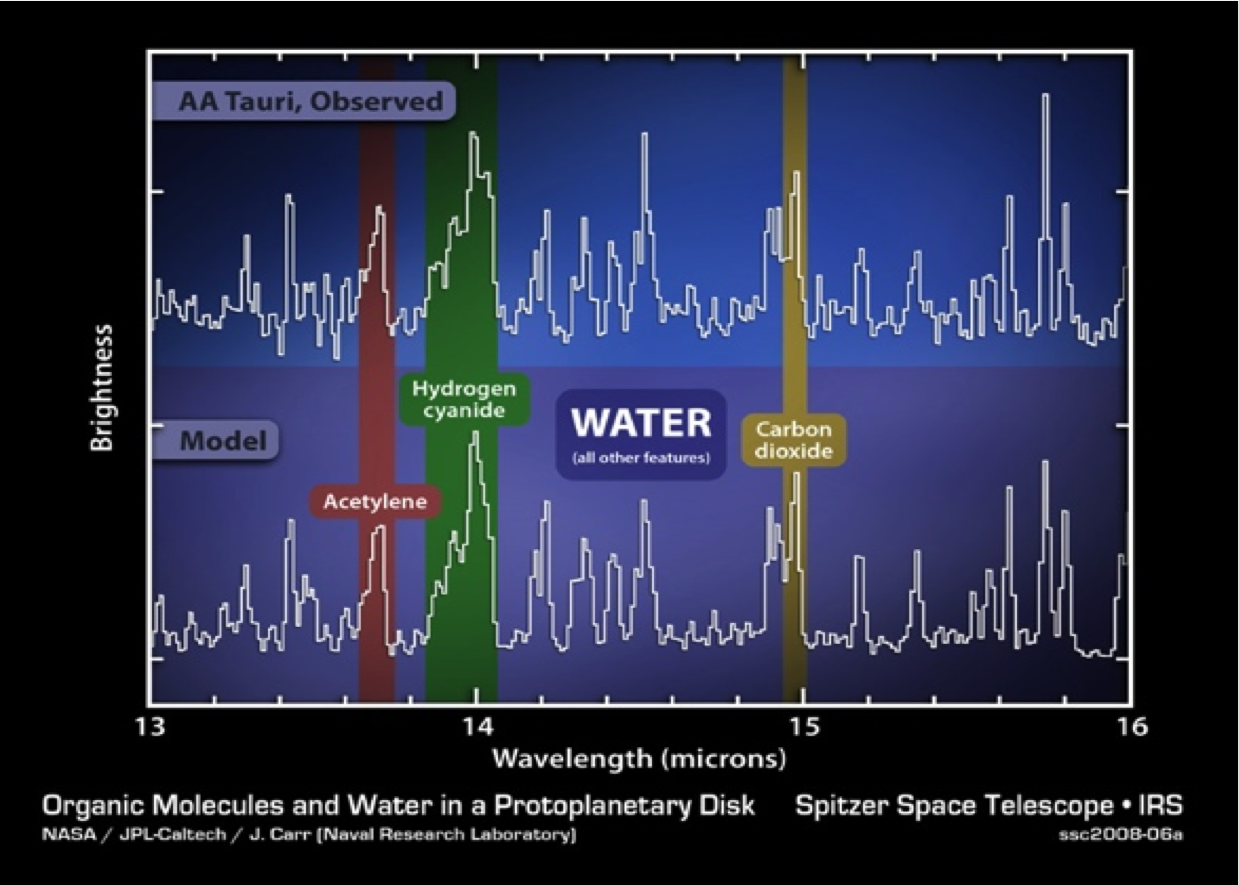
\includegraphics[width=0.8\textwidth]{figures/spitzer.png}
%%\vspace{-0.5in}
%\caption{Spitzer IR spectrum of the disk around AA Tauri showing detections of acetylene, hydrogen cyanide, carbon dioxide and water.}
%\label{fig:spitzer}
%\end{figure}

\begin{figure}[h]
\centering
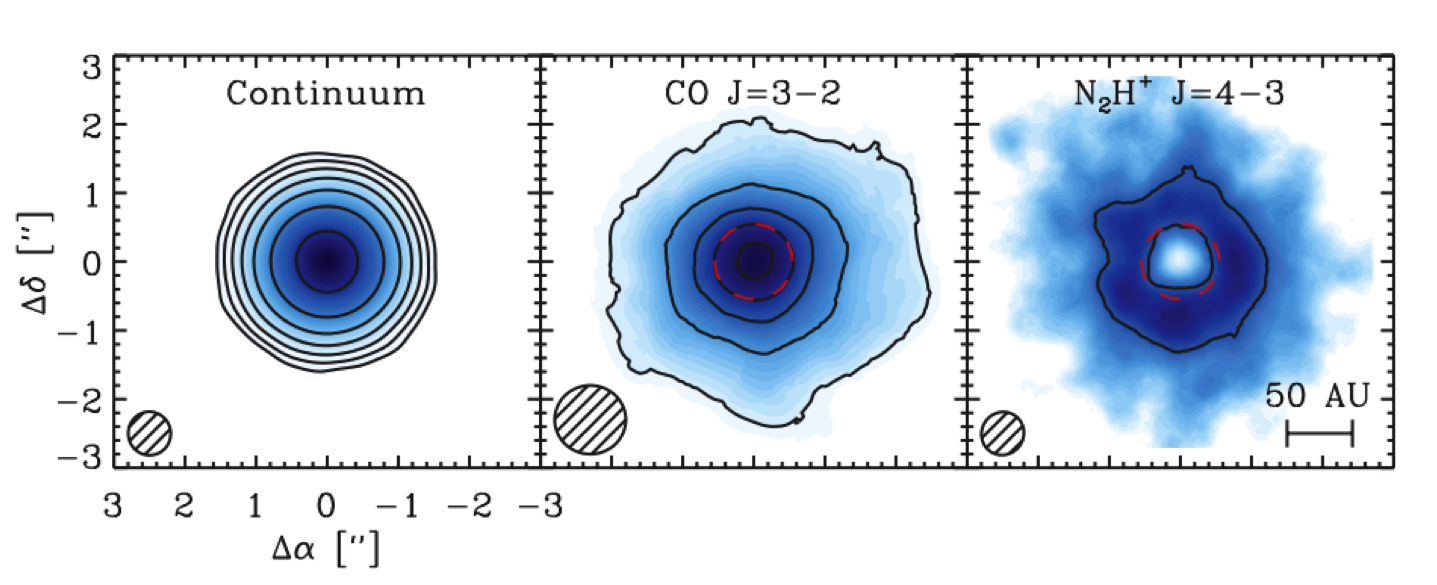
\includegraphics[width=0.8\textwidth]{figures/CO.png}
%\vspace{-0.5in}
\caption{ALMA detection of the CO snowline in TW Hya at 30 AU. Reprinted with permission from \citet{qi13}.}
\label{fig:qi13}
\end{figure}

%\begin{figure}[t!]
%\centering
%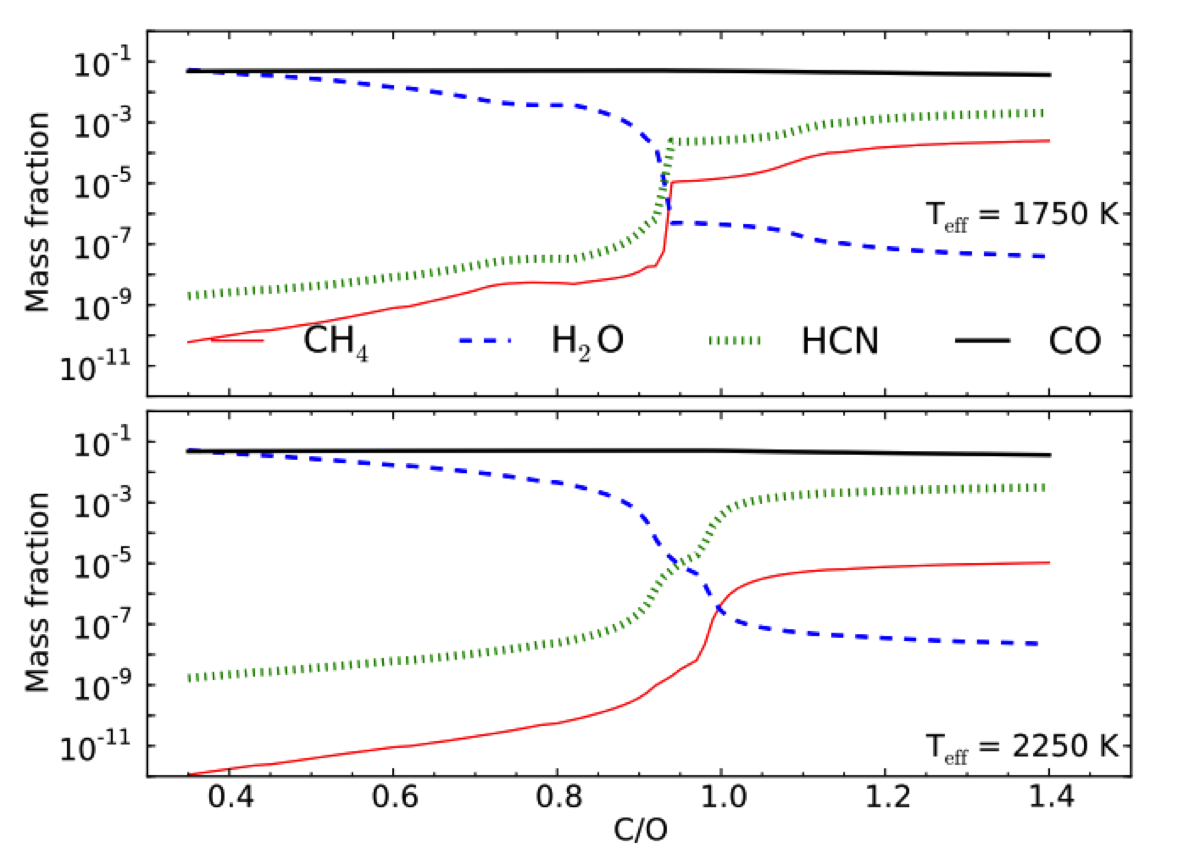
\includegraphics[width=0.8\textwidth]{figures/molliere.png}
%%\vspace{-0.5in}
%\caption{Theoretical model of an exoplanet atmosphere showing that small variations in the C/O ratio produce very large variations in the abundance of other volatiles. From \citet{molliere15}.}
%\label{fig:molliere}
%\end{figure}

%\subsubsection{C/O Ratios in Disks}

One important effect of the existence of snowlines is that disks are expected to contain different amounts of volatiles in gas and in dust at different locations. As the main carbon and oxygen carriers, i.e. H$_2$O, CO$_2$ and CO, are amongst the most abundant volatiles in comets and protostellar cores (\citealt{rodgers02}, \citealt{mumma11}, \citealt{henning13}), variations in the carbon-to-oxygen (C/O) ratio in gas and dust throughout a disk are particularly important. This issue was first addressed by \citet{oberg11}. Figure \ref{fig:oberg} shows the C/O ratio in gas and dust as a function of semimajor axis, assuming protostellar abundances for the volatiles. The C/O ratio in gas is enhanced compared to the stellar value, particularly between the CO$_2$ and CO snowlines where it reaches unity. The pioneering work of \citet{oberg11} inspired Chapter 4 of this thesis. \citet{oberg11} consider a static disk, and thus do not account for dynamical processes such as redistribution of solids due to radial drift, the radial movement of the nebular gas, and accretion heating. We expand this model by considering the processes outlined above and their effect on snowline locations. In particular, we focus on how radial drift of solids and viscous gas accretion onto the central star affect the H$_2$O, CO$_2$ and CO snowline locations for particles of different sizes. %We find that drift and accretion heating alone may move the snowlines inward by factors of $\sim$2 compared to a static disk, thus substantially changing the disk regions with enhanced gas-phase C/O ratios. %, which has direct consequences for planet formation. 

\begin{figure}[h]
\centering
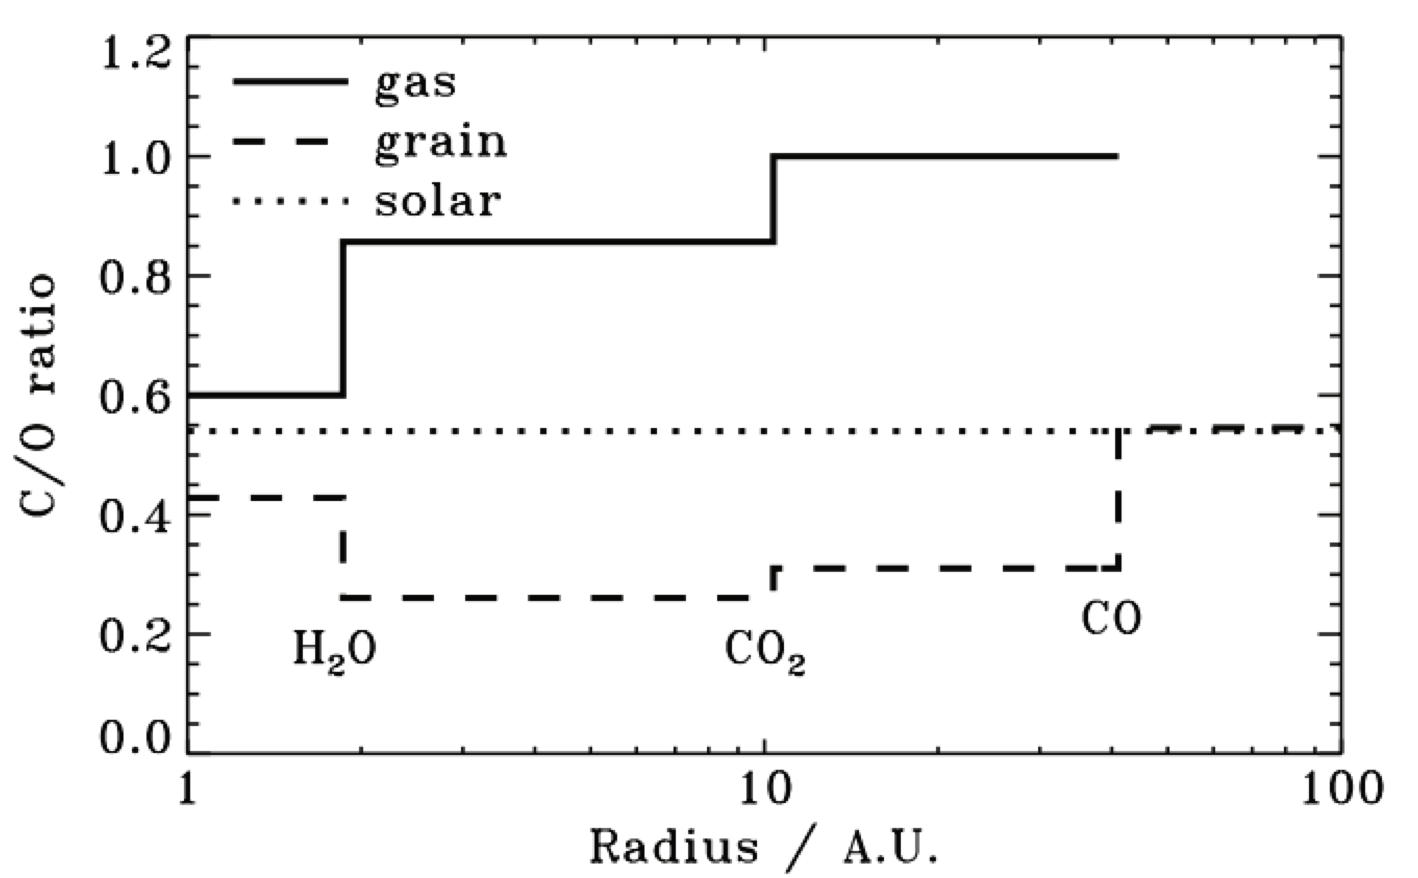
\includegraphics[width=0.8\textwidth]{figures/oberg11.png}
%\vspace{-0.5in}
\caption{The C/O ratio in gas (solid line) and dust (dashed line) as a function of semimajor axis in a static disk. The dotted line shows the stellar value of 0.54. Gas-phase C/O ratios of order unity can be achieved in the outer disk. Reprinted with permission from \citet{oberg11}. }
\label{fig:oberg}
\end{figure}



%\subsubsection{The Importance of Nitrogen}

As we show above, the C/O ratio is highly important to study, but it only provides us with one piece of the puzzle that is disk gas and grain elemental compositions in dynamic disks. In order to improve our theoretical models, we thus need to look at other molecules and volatile compounds. The first that comes to mind is nitrogen, as it highly abundant in the Solar System \citep{lodders03}, and primarily believed to exist as N$_2$ (e.g., \citealt{owen01}). Molecular nitrogen cannot be detected directly. However, an inventory of nitrogen cometary abundances shows that NH$_3$ is the most abundant observed nitrogen carrier, and yet its concentration is only a small fraction of the total nitrogen abundance, which leaves N$_2$ as the main nitrogen bearing species. In the context of planet compositions, N$_2$ is important due to its high volatility. The gas phase
nitrogen-to-oxygen (N/O) ratio in the outer disk may thus be even more enhanced than the C/O ratio. %We calculate the N/O ratio in gas and dust in Chapter 5, and confirm that it is indeed highly enhanced compared to the stellar value throughout most of the disk.

%We note that this differential volatile condensation effect has already been used to explain potential claims hat some planets, such as WASP-12 b, have a superstellar C/O ratio \citep{madhu11}. While this particular detection has since been unequivocally refuted (e.g., \citealt{kreidberg15}), the advent of JWST in the near future will provide us with a significantly larger sample of atmospheric spectra which may be used to constrain C/O ratios in other giant planet atmospheres. 
%
%
%
%While there are several volatiles in disks that can be further investigated, one important signature of atmospheric chemistry is the carbon-to-oxygen (C/O) ratio. This is demonstrated in Figure \ref{fig:molliere}, which shows a theoretical model of an exoplanet atmosphere: variations in the C/O ratio by factors of $\sim$3 change the abundance of other volatiles, such as H$_2$O and CH$_4$ by several orders of magnitude. From the observational perspective, an exciting potential discovery was that some planets, such as WASP-12 b, have a superstellar C/O ratio \citep{madhu11}. While this particular detection has since been unequivocally refuted (e.g., \citealt{kreidberg15}), the advent of JWST in the near future will provide us with a significantly larger sample of atmospheric spectra which may be used to constrain C/O ratios in other giant planet atmospheres. The possibility of a superstellar C/O ratio in a disk or planet atmosphere is also intriguing from a theoretical standpoint. One likely explanation is that the main carbon and oxygen carriers, i.e. H$_2$O, CO$_2$ and CO, have different condensation temperatures. This will result in variations in the abundance of the volatiles in gas and solid form between their respective snowlines, which will subsequently change the C/O ratio at different disk radii. This idea was first postulated by   



%\subsection{Ice Morphology}


The snowline locations of volatiles, including carbon, oxygen and nitrogen carriers, are highly dependent on the morphology of the icy particles. These can either be mixed ices or layered ices, where each ice layer is pure (e.g., \citealt{pontoppidan03}). As H$_2$O is the least volatile species with high abundance in disks, one can typically expect the more volatile molecules to form on a water substrate (but see \citealt{bisschop06} for other scenarios). In some environments the more volatile species may form a thick enough layer on top of the water ices that they essentially behave as pure ices, however. The ice environment in which the molecules reside, i.e. pure or water dominated ices, will determine their binding energies. This, in turn, will change the temperatures at which the ices desorb, and thus their snowline locations. This effect is particularly important in the case of CO and N$_2$, since their volatility is significantly higher than that of other carbon and nitrogen carriers, such as CO$_2$ or NH$_3$. Laboratory experiments \citep{fayolle16} have determined new values for the CO and N$_2$ binding energies, both as pure ices and water dominated. Figure \ref{fig:fayolle} shows the results of a temperature programmed desorption (TPD) experiment for the CO and N$_2$ desorption rate as a function of temperature, in water dominated and pure ice environments. The peak of the desorption curves shifts considerably between the different binding environments. This translates into a difference in binding energies by up to a factor of two between pure and water dominated CO or N$_2$. %We show in Chapter 5 that this large difference in binding energies changes the CO and N$_2$ snowline locations by factors of 3-4 spending on the ice environment. By taking into account also the effect of disk dynamics, we find that the CO and N$_2$ snowlines may span several tens of AU. This uncertainty in snowline locations suggests yet again that more observations are needed to constrain disk volatile compositions at different locations. %, and thus trace the origins of gas giants based on their atmospheric compositions.  

\begin{figure}[t!]
\centering
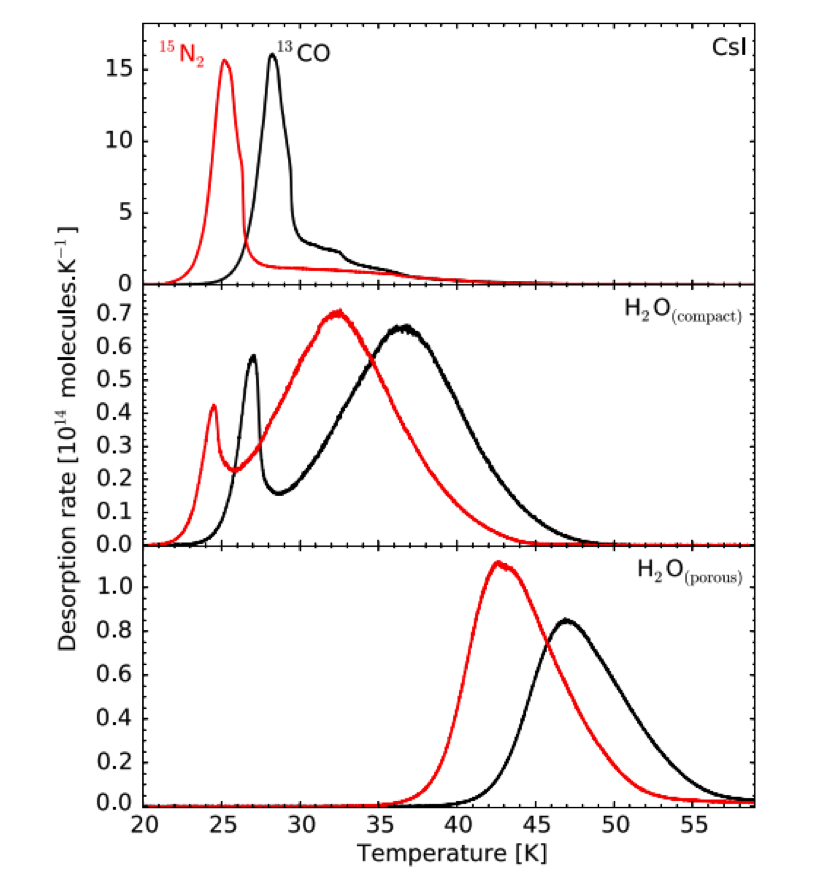
\includegraphics[width=0.8\textwidth]{figures/fayolle.png}
%\vspace{-0.5in}
\caption{Desorption rate as a function of temperature in a TPD experiment, for CO and N$_2$ as pure ices (top panel), on a compact H$_2$O substrate (middle panel), and on porous H$_2$O substrate (bottom panel). The peaks in the desorption curves are at substantially higher temperatures for the water dominated ices. Reprinted with permission from \citet{fayolle16}.}
\label{fig:fayolle}
\end{figure}





   


   

%\subsection{The Role of Disk Location in Setting the Minimum Core Mass for Giant Planet formation}
%
%\begin{itemize}
%
%\item Gas giants are largely believed to form through core accretion (insert core accretion sketch from various talks). This process is particularly challenging in the outer disk due to long dynamical timescales. At the same time, wide separation gas giants have been discovered (HR 8799 plot). This poses an intriguing question: how do these planets form: I answer this question in the first part of my thesis; specifically I calculate the minimum Mcrit, which applies when cores no longer accrete solids. Standard core accretion studies are not built to properly explore this Mcrit. Here explain standard core accretion studies in more detail and insert e.g. one of the Mass vs time figures from Pollack et al. 1996. Explain how our study is different. Finalize by saying that the studies I performed clearly challenge previous claims that  core accretion cannot operate at wide separations, thus reopening the case for in-situ formation of wide separation gas giants.
%
%\end{itemize}
%
%\subsection{The Role of Disk Dynamics and Morphology in Setting Snowline locations and C/N/O Ratios}
%
%\begin{itemize}
%
%\item Disk Composition Regulates Planet Composition. It is thus essential to (1) predict what kinds of planet compositions result from planet location in different parts of the disk, and (2) conversely, bacl-track planet formation location based on planet composition.
%
%\item Disks are complex. Show figure from Henning and Semenov with all processes that occur in disks and discuss which ones I tackle in the thesis.
%
%\item However, we do know some things about disks. Volatile molecules have detected in disks (show figure with Spitzer IR spectrum of AA Tauri). Snowlines have also been detected (show CO snowline plot from Qi+13).
%
%\item One important signature of atmospheric chemistry is the C/O ratio (explain why and show plot from Molliere+15 which shows the effect of varying C/O ratio on the abundance of other volatiles). Discuss claims that super stellar C/O ratios have been detected (show Wasp 12-b spectrum from Madhusudhan), but have since been refuted. Explain that this poses an intriguing question from a theoretical standpoint. Mention idea proposed by Oberg+11 (show plot). Discuss that disk dynamics have an important role, which is partly what we tackle in this part of the thesis.
%
%\item There are other important volatiles besides H2O, CO2 and CO. Discuss the importance of N2 and show plot with abundances in comets that show that NH3 is the main carrier based on observations, but it doesn't account for all the nitrogen in the solar system. 
%
%\item Ice morphology is important. Discuss why. Discuss how binding energies depend on the ice environment and show plot from Edit's paper. 
%
%\item It follows that we have to take into account additional volatiles, abundances and ice morphologies besides disk dynamics to see their effect on snowline locations and the C/N/O ratios. We tackle this in Chaper xx.
%
%\item We demonstrate in this part to the thesis that C/N/O ratios may be used to track a planet's formation origin, when combined with observations, but that more observations are needed.
%
%\end{itemize}

\section{The Disk-Planet Connection}

\subsection{Consequences of Different Disk C/N/O Ratios on Planetary Atmospheres}

Variations in the C/O ratio in gas and dust due to different volatile condensation temperatures have also been investigated in exoplanet atmospheres, both from a theoretical and observational standpoint. \citet{molliere15} show that varying the C/O ratio in a gas giant envelope by factors of $\sim$3 changes the abundance of other volatiles, such as H$_2$O and CH$_4$, by several orders of magnitude. From the observational perspective, an exciting potential discovery was that some planets, such as WASP-12 b, have a superstellar C/O ratio \citep{madhu11}. While this particular detection has since been unequivocally refuted (e.g., \citealt{kreidberg15}), the advent of JWST in the near future will provide us with a significantly larger sample of atmospheric spectra which may be used to constrain C/O ratios in other giant planet atmospheres. 

While observational constraints for the N/O ratio in planetary atmospheres do not currently exist, the high gas-phase N/O ratio enhancement at most disk radii suggests that giant planets that form at wide separations should have an excess of nitrogen in their atmospheres, which could be used to trace their formation origin. Theoretical and observational knowledge of both C/O and N/O ratios could further help back-track the planet formation location based on planet composition. 



\subsection{Thesis Outline}

This thesis is organized as follows. In Chapter 2, we determine the minimum core mass for giant planet formation for a range of disk radii, using idealized assumptions about the properties of the nebular gas and of the dust grains. We expand this model in Chapter 3, where we calculate this minimum core mass assuming a realistic gas equation of state and realistic opacities. In Chapter 4, we explore the role of disk dynamics in setting the snowline locations of the main carbon and oxygen carriers, and the consequences for the C/O ratio in gas and dust throughout the disk, as well as for the compositions of giant planets forming at different radii. Finally, we expand this model in Chapter 5 by considering additional volatile species and different ice morphologies. 

%where we find that the minimum core mass for giant planet formation is lower than the one typically quoted, 10 $M_{\oplus}$ (\citealt{stevenson82}, \citealt{rafikov06}), and may be as low as 1 $M_{\oplus}$. Our study thus reopens the case for in situ formation of wide-separation gas giants through core accretion.

Our work in the two main parts of this thesis (Chapters 2 \& 3, and 4 \& 5, respectively) confirms that there is indeed a tight link between disks and planets. Our study on core accretion shows that the core mass required to form a gas giant is highly dependent on the disk properties and composition, while our chapters on snowline locations and C/N/O ratios also demonstrate that the disk structure and chemical composition has direct effects on the volatile composition of giant planets atmospheres. This thesis thus sets the stage to uncovering the role of disk volatile composition, dynamics and chemistry in shaping the compositions of nascent giant planets. 




%\begin{savequote}[75mm]
%Nulla facilisi. In vel sem. Morbi id urna in diam dignissim feugiat. Proin molestie tortor eu velit. Aliquam erat volutpat. Nullam ultrices, diam tempus vulputate egestas, eros pede varius leo.
%\qauthor{Quoteauthor Lastname}
%\end{savequote}

\chapter{On the Minimum Core Mass For Giant Planet Formation at Wide Separations}
%
%\newthought{There's something to be said} for having a good opening line. Morbi commodo, ipsum sed pharetra gravida, orci  $x = 1/\alpha$ magna rhoncus neque, id pulvinar odio lorem non turpis \cite{Eigen1971, Knuth1968}. Nullam sit amet enim. Suspendisse id velit vitae ligula volutpat condimentum. Aliquam erat volutpat. Sed quis velit. Nulla facilisi. Nulla libero. Vivamus pharetra posuere sapien. Nam consectetuer. Sed aliquam, nunc eget euismod ullamcorper, lectus nunc ullamcorper orci, fermentum bibendum enim nibh eget ipsum. Donec porttitor ligula eu dolor. Maecenas vitae nulla consequat libero cursus venenatis. Nam magna enim, accumsan eu, blandit sed, blandit a, eros.
%$$\zeta = \frac{1039}{\pi}$$
%

\section*{Abstract}

In the core accretion hypothesis, giant planets form by gas accretion onto solid protoplanetary cores.  The minimum (or critical) core mass to form a gas giant is typically quoted as $10 M_{\oplus}$. The actual value depends on several factors: the location in the protoplanetary disk, atmospheric opacity, and the accretion rate of solids. Motivated by ongoing direct imaging searches for giant planets, this study investigates core mass requirements in the outer disk.  To determine the fastest allowed rates of gas accretion, we consider solid cores that no longer accrete planetesimals, as this would heat the gaseous envelope. Our spherical, two-layer atmospheric cooling model includes an inner convective region and an outer radiative zone that matches onto the disk.  We determine the minimum core mass for a giant planet to form within a typical disk lifetime of 3 Myr.   The minimum core mass declines with disk radius, from $\sim$$8.5 M_{\oplus}$ at 5 AU to $\sim$$3.5 M_{\oplus}$ at 100 AU, with standard interstellar grain opacities.  Lower temperatures in the outer disk explain this trend, while variations in disk density are less influential.  At all distances, a lower dust opacity or higher mean molecular weight reduces the critical core mass. Our non-self-gravitating, analytic cooling model reveals that self-gravity significantly affects early atmospheric evolution, starting when the atmosphere is only $\sim$$10\%$ as massive as the core.

\noindent The contents of this chapter are published in \textit{Piso, A.-M. A \& Youdin, A. N. Y}

\section{Introduction}
\label{intro}

Models of giant planet formation fall in two categories:  core accretion or gravitational instability \citep{dangelo11, youdin13}. In core accretion models, a solid core grows until it becomes massive enough to rapidly accrete gas \citep{PerCam74, mizuno78}.  Gravitational instability (GI) theories investigate the fragmentation of the protoplanetary disk into bound clumps \citep{cameron78, boss97}. 

Forming giant planets at wide separations in the protoplanetary disk poses theoretical challenges for both models.  While disks cannot fragment close to their host star, GI is more promising in the outer disk \citep{matzner05, rafikov05}.   However,  for GI to form planetary mass objects versus brown dwarfs, both instantaneous disk conditions and the history of gas infall must be finely tuned \citep{kratter10}.  The main concern for core accretion models, which are successful in the inner disk, is that they operate too slowly in the outer disk. The few Myr lifetime of gas disks sets the constraint \citep{williams11}.  However, mechanisms for the rapid accretion of solids, even at large separations, exist \citep{dones93, kenyon09, lambrechts12}. We thus consider the complementary problem of gas accretion timescales in the outer disk.

Core accretion models fall in several categories: static, quasi-static evolutionary and hydrodynamic.
In static models, the accretion of planetesimals provides a steady luminosity that determines the structure and mass of the atmosphere \citep{stevenson82}.    For a given planetesimal accretion rate, static solutions only exist up to a maximum core mass, referred to as the ``critical core mass",  $\MC$. Above this mass, the atmosphere is assumed to collapse and rapidly accrete disk gas, a process known as the ``core accretion instability."

Many static studies reproduce a canonical $\MC \sim 10 M_\oplus$.  However, \citet[hereafter R06]{Raf11, rafikov06} finds a wide range of values, $0.1 M_\oplus \lesssim \MC \lesssim 100 M_\oplus$, depending on the planetesimal accretion rate and disk parameters. % \citep[see also][]{Raf11}.  
Section \ref{sec:placc} compares our results to R06.  A general limitation of static models is the neglect of heat generated by atmospheric collapse, which can transform the core accretion instability into a slower process of Kelvin-Helmholtz (KH) contraction.

Quasi-static models include time-dependent atmospheric evolution due to KH contraction, and typically include a time-varying planetesimal accretion rate \citep{boden86, alibert05}.   Successful quasi-static models describe three phases of giant planet formation \citep{pollack96}.  In phase 1, rapid planetesimal accretion gives significant core growth, but prevents the accretion of a massive atmosphere.  When planetesimal accretion abates, as the core's feeding zone is depleted of solids, phase 2 begins.  During phase 2, the atmosphere grows gradually, cooling by KH contraction.  An ongoing trickle of planetesimal accretion can heat the atmosphere and slow this contraction.  Eventually, the atmosphere reaches the ``crossover mass", when it equals the mass of the now slowly growing core.  Phase 3, the runaway growth of the atmosphere, begins around the crossover mass.  This runaway occurs quasi-statically, i.e.\ in hydrostatic balance, but very rapidly compared to disk lifetimes. 

Dynamical models are needed to understand how runaway growth ends and final planet masses are determined.  Relevant processes -- including gap opening in disks and the transition of accretion from spherical to planar -- can be simulated and then added to atmospheric evolution calculations \citep{LisHub09}.

This work develops quasi-static models in which the core has a fixed mass and is no longer accreting solids.  By isolating the process of KH contraction, we determine the minimum timescale for runaway atmospheric growth, and thus for giant planet formation by core accretion.  Previous studies have considered this type of growth \citep[hereafter I00; PN05, respectively]{ikoma00, pn05}, which is an end-member case of phases 2 and 3 in more detailed quasi-static models.  Especially since phase 2 of atmospheric growth is often the slowest stage of core accretion, understanding the fastest allowed rates of gas accretion is of crucial importance.  Our study develops simplified cooling models for the purposes of broadly exploring parameter space -- especially in the outer disk -- and developing a more detailed understanding of atmospheric accretion.

This paper is organized as follows. Section \S\ref{sec:model} describes our model of atmospheric growth.  In Section \S\ref{sec:coolingan}, we develop a simplified analytic version of our atmospheric model.  We describe the structure and evolution of our atmosphere solutions in Section \S\ref{sec:KH}.   Section \S\ref{sec:critical} gives our final results for growth timescales and critical core masses.  We discuss some neglected effects in Section \S\ref{sec:neglected} and summarize our findings in Section \S\ref{sec:conclusions}.  Some detailed derivations are presented in the appendices.


\section{Atmospheric Accretion Model} \label{sec:model}

To model the accretion of gas by a solid protoplanet, we develop a simplified two-layer model for time-dependent atmospheric growth via cooling, i.e. KH contraction.  With a convective interior and radiative exterior, this model is motivated by similar models of hot Jupiters \citep{ab06, ym10}. 

Our model can  treat atmospheric growth up to the early stages of runaway growth, around the crossover mass.  At higher masses, our approximate treatment of the radiative zone (explained below) breaks down.   Since evolution after the onset of runaway growth contributes minimally to the total planet formation timescale, we can model growth times to good accuracy. 
%Our treatment is also inappropriate for hot, short-period planets, where dust sublimation gives deeper radiative zones that require more detailed models.

Our main assumptions are summarized as follows:
\begin{enumerate}
\item The atmosphere is spherically symmetric, remains in hydrostatic balance, and matches onto the disk's midplane temperature and pressure at the planet's Hill radius.
\item The core mass and radius are fixed in evolutionary calculations, neglecting ongoing planetesimal or dust accretion.
%\item At the planet's Hill radius, the atmospheric temperature and pressure match the conditions in the disk midplane.
\item Gravitational contraction of the atmosphere is the only source of planetary luminosity.  
\item Cooling of the atmosphere is dominated by the convective interior.  Thus the luminosity in the radiative exterior is held spatially constant. We justify this assumption in \S\ref{sec:twolayer} and confirm its validity in \S\ref{sec:endoftime}.
%\item A global cooling model connects independent static solutions into a time-dependent sequence.
\item The atmosphere obeys a polytropic equation of state (EOS), with adiabatic index $\gamma = 7/5$ for an ideal diatomic gas.  Corrections from a realistic EOS are discussed in \S\ref{sec:EOS} and deferred to future work.
\item Dust grains provide the opacity in the radiative zone. For the cool temperatures in the outer disk, the radiative layer remains cool enough to avoid dust sublimation. Other opacity choices are discussed in \S\ref{sec:op}.
%\item Because gas accretion accelerates after the crossover mass, the time to reach the crossover mass, i.e. the crossover time, is a good approximation of the total time to form a gas giant.
\end{enumerate}
%The remainder of this section develops our model in more detail.

The first assumption of spherical accretion breaks down early in the inner disk, as explained below.  However, our focus is on the outer disk, where this standard approximation is better justified.

\subsection{Disk and Opacity Model}\label{sec:disk}

We adopt a minimum mass solar nebula (MMSN) model for a passively irradiated disk \citep{chiang10}. With the semimajor axis $a$ normalized to the outer disk as $\aun{10} = a/(10 \text{ AU})$, the gas surface density and mid-plane temperature are  
\begin{subeqnarray} \label{eq:diskparam}
\varSigma\di  &=& 70 \,F_\varSigma \aun{10}^{-3/2} ~{\rm g~cm}^{-2} \\
T\di &=& 45  \,F_T\, \aun{10}^{-3/7} ~{\rm K} \, .
%\Sigma\di&=&2200 F_{\Sigma} a^{-3/2}\,\, \text{g cm}^{-2} \slabel{eq:diska}\\
%T\di &=& 120 F_T a^{-3/7} \, \text{K}, \slabel{eq:diskb}
\end{subeqnarray}
The normalization factors $F_{\Sigma}$ and $F_T$  adjust the model relative to the fiducial MMSN.  We fix $F_{\varSigma}=F_T=1$ unless noted otherwise.  Some observations support a flatter surface density profile, $\varSigma\di \propto a^{-1}$ \citep{andrews10}.  We find that gas density and pressure are weak corrections to atmospheric growth (see Section \S\ref{sec:critical}).  However, a greater surface density of solids in the outer disk could favor the rapid growth of cores \citep{bromley11}.

For a vertically isothermal disk in hydrostatic balance (with no self-gravity), the mid-plane pressure of disk gas is 
\begin{equation}
\label{eq:Pd}
P\di = 6.9 \times 10^{-3} F_\varSigma \sqrt{F_T} \, \aun{10}^{-45/14}~{\rm dyn~cm^{-2}}
%P\di=1.1 \times 10^{-4} F_{\Sigma} \sqrt{F_T} a^{-45/14} \,\, \text{dyne cm}^{-2} %\times \sqrt{m_\ast}
\end{equation}
for a molecular weight of $\mu=2.35$ proton masses and a Solar mass star.  %Changes to the stellar mass (not considered here) would affect both the dynamic mass and, by heating the disk, $T\di$.
%The fiducial pressure is a paltry 7 nanobars.

The (thermodynamically isothermal) sound speed in the disk is
\begin{equation}
c\di = \sqrt{\Rg T\di} = 0.4 \sqrt{F_T} \aun{10}^{3/14} ~\text{km s}^{-1} \,,
\end{equation}  
in terms of the specific gas constant $\Rg$.  The disk scale height is 
\begin{equation}
H\di = {c\di / \varOmega} = 0.42 \sqrt{F_T}  \, \aun{10}^{9/7} \AU\, ,
\end{equation} 
in terms of the Keplerian frequency $\varOmega = \sqrt{G M_\ast/a^3}$, with $G$ the gravitational constant and $M_\ast$ the stellar (in this work Solar) mass. 

We assume a dust opacity characteristic of interstellar grains, following \citet{bell94}:
\begin{equation}
\label{eq:opacitylaw}
\kappa= 2 F_\kappa  \left(\frac{T}{100\; \rm{K}}\right)^{\beta} \; \mathrm{cm^2 ~ g^{-1}},
\end{equation}
with a power-law index $\beta = 2$ and normalization $F_\kappa = 1$ unless noted otherwise. Grain growth tends to lower both $F_\kappa$ and $\beta$, while dust abundance scales with $F_\kappa$.   Section \S\ref{sec:op} discusses dust sublimation and more realistic opacity laws.


\subsection{Length Scales}
\label{sec:scales}

The characteristic length scales for protoplanetary atmospheres are crucial for choosing boundary conditions and for understanding the validity of  spherical symmetry in a gas disk of scale height $H\di$.

The solid core has a radius
\begin{equation}
\label{eq:rc}
R\co \equiv \left(\frac{3 M\co}{4 \pi \rho\co}\right)^{1/3} \approx 10^{-4} \mcn{10}^{1/3} ~\text{AU},
\end{equation}
where the core mass, $M\co$, is normalized to 10 Earth masses as $\mcn{10} \equiv M\co/(10~M_\oplus)$. The core density is held fixed at $\rho\co=3.2$ g cm$^{-3}$, representing a mixture of ice and rocky material \citep{pap99}.  We thus neglect  the detailed EOS of the solid core \citep{fortney07}.

A planet can bind a dense atmosphere if its escape velocity exceeds the sound speed.  This criterion is satisfied inside the Bondi radius
\begin{equation}
\label{eq:RB}
\RB \equiv \frac{G M\pla}{c\di^2} \approx 0.17 \, {\mpn{10}  \, \aun{10}^{3/7} \over F_T} ~\AU,
\end{equation}
where the enclosed planet mass, $M\pla = M\co + M_\mathrm{atm}$, includes the core and any atmosphere within the Bondi radius and $\mpn{10} \equiv M\pla /(10~M_\oplus)$.   The contribution of the atmospheric mass is small in early evolutionary stages.

Stellar tides dominate the planet's gravity beyond the Hill radius
\begin{equation}
\label{eq:RHill}
R_{\rm H} = \left(M\pla \over 3 M_\ast \right)^{1/3}a \approx 0.22 \, {\mpn{10}^{1/3} \, \aun{10} }~\AU ,
\end{equation}
where spherical symmetry and hydrostatic balance break down.  (Here we use the same symbol, $M\pla$, to now mean the mass within $\RH$.) 

The relevant length scales of the atmosphere and disk satisfy the relation $\RB H\di^2 = 3 R_{\rm H}^3$.  The length scales are roughly equal at the ``thermal mass'' (e.g., \citealt{menou04})
\begin{equation}\label{eq:Mth}
M_{\rm th} > {c\di^{3} \over G \varOmega} \approx 25 \, {F_T^{3/2} \over \sqrt{m_\ast} } \, \aun{10}^{6/7}~ M_\oplus \, .
\end{equation} 

In the low mass regime, $M\pla < M_{\rm th}/\sqrt{3}$, the length scales order as $\RB< \RH<H\di$.  In this regime, many studies assume the atmosphere matches the disk conditions at $\RB$.  We use $\RH$ as the matching radius, i.e.\ outer boundary, in all regimes. We discuss this choice further below.  
%\textbf{This choice reflects the fact that, even outside the Bondi radius, hydrostatic densities exceed the background density (see R06). Nevertheless, since the density contrast is modest outside $\RB$, these two boundary conditions give similar results.  We do not extend our models past $\RH$, where tidal forces dominate. }

 %We are accounting for the fact that, in hydrostatic models, the density at 
 %$\RB$ is higher than the background density (see R06). Nevertheless, since the density change is modest, these two boundary conditions give similar results. 

For a finite range of intermediate masses, $M_{\rm th}/\sqrt{3} < M\pla < 3 M_{\rm th}$, the Hill radius is the smallest scale, satisfying both $\RH < \RB$ and $\RH < H\di$.  Spherical symmetry remains a good, if imperfect, approximation because the disk is only weakly vertically stratified on  scales $\lesssim H\di$.  

At higher planet masses where $M\pla > 3 M_{\rm th}$ and $H\di < \RH < \RB$, spherical symmetry is no longer a good approximation, due to both the vertical stratification of the disk and gap opening.  See \S\ref{sec:hydro} for further discussion of neglected hydrodynamic effects.

We quote planet masses as the enclosed mass within the smaller of $\RB$ and $\RH$.  Thus when $\RB < \RH$, our computational domain -- which always ends at $\RH$ -- extends further than the location where we define atmosphere mass, within $\RB$.  We emphasize that this mass definition does not affect the evolutionary calculation, which consistently includes the enclosed mass at all radii.   We justify our mass convention as follows.  First, we want to conservatively define planet mass in a way that does not exaggerate atmospheric growth and is more consistent with previous works that use $\RB$ as the outer boundary in this regime (e.g., \citealt{ikoma00}, \citealt{pollack96}).  Second, most of the gas outside $\RB$ is weakly bound, and unlikely to remain attached to the planet if the disk suddenly dissipates.

The choice of $\RH$ as the outer boundary is based on this being the largest radius where spherical hydrostatic balance is approximately (but not exactly, see \S\ref{sec:hydro}) valid.  When $\RB < \RH$, we thus include the fact that the density at $\RB$ slightly exceeds the background disk density (see R06).  In practice, this effect is not very significant.  We would get similar results by choosing the outer boundary at $\RB$ in this regime, as previous studies have done.

 %  This conservative choice in quoting planet masses is usually a minor distinction because (when $\RB < \RH$) the gas between $\RB$ and $\RH$ is weakly compressed.

%\textbf{Finally, the mass at which core growth rapidly decreases due to depletion of planetesimals from the core's feeding zone is called the isolation mass. For our fiducial disk model and for an assumed dust-to-gas ratio of 0.01, the isolation mass is given by}
%
%\begin{equation}
%\label{eq:Misol}
%M_{\rm isol} \sim 2 \pi a \times 2 \RH \times \Sigma_{\rm p} \approx 0.2 a_{10}^{3/4} ~ M_{\oplus},
%\end{equation}
%\textbf{where $\Sigma_p$ is the surface density of solids. Since in our regime the core is no longer accreting solids, we require $M_{\rm isol}$ to always be smaller than the core mass at which runaway gas accretion commences, i.e. the critical core mass.}

\subsection{Structure Equations and Boundary Conditions}
\label{sec:struct}

Our atmosphere calculations use the standard structure equations of mass conservation, hydrostatic balance, thermal gradients, and energy conservation:
\begin{subeqnarray}
\label{eq:struct}
\frac{dm}{dr}&=&4 \pi r^2 \rho\slabel{eq:structb} \\
\frac{dP}{dr}&=&-\frac{G m}{r^2}\rho \slabel{eq:structa} \\
\frac{dT}{dr}&=&\nabla \frac{T}{P}\frac{dP}{dr}\slabel{eq:structc} \\
\frac{dL}{dr}&=&4 \pi r^2 \rho \left(\epsilon - \left. T {\partial S \over \partial t} \right|_m \right)\slabel{eq:structd}, 
\end{subeqnarray}
\noindent where $r$ is the radial coordinate, $L$ is the luminosity, and $P$, $T$, $\rho$  and $S$ are the gas pressure, temperature, density and entropy, respectively.  The enclosed mass  at radius $r$ is $m$. \Eq{eq:structc} simply defines the temperature gradient  $\nabla \equiv d \ln T/d \ln P$.  

Radiation diffusion gives a temperature gradient
\begin{equation}
\label{eq:delrad}
\delrad \equiv \frac{3 \kappa P}{64 \pi G m \sigma T^4} L\, ,
\end{equation}
with $\sigma$ the Stefan-Boltzmann constant.  In our models, optically thick diffusion is a good approximation throughout the radiative zones.  In convectively unstable regions, efficient convection gives an isentropic temperature gradient with $\nabla = \delad$, the adiabatic gradient 

\begin{equation}
\label{eq:delad}
\delad \equiv \Big(\frac{d \ln T}{d \ln P}\Big)_{\rm{ad}}.
\end{equation}
According to the Schwarzschild criterion, convective instability occurs when $\delrad > \delad$.  Thus $\nabla = \min(\delrad, \delad)$ sets the temperature gradient.

In the energy equation (\ref{eq:structd}), $\epsilon$ represents all local sources of heat input, except for the motion of the atmosphere itself.  From stellar structure, $\epsilon$ may be familiar as a nuclear burning term.  In a protoplanetary atmosphere, dissipative drag on planetesimals contributes to $\epsilon$.  Our models set $\epsilon = 0$, consistent with our neglect of planetesimal accretion.

The energy input from gravitational contraction, $\epsilon_{\rm g} = -T \partial S / \partial t$, is crucial for a cooling model.\footnote{In general, any motion is accounted for by this term.  The partial time derivative is performed on shells of fixed mass.}  The partial time derivative would normally require our radial derivative to be partial as well.  However, our subsequent developments will replace the local energy equation (\ref{eq:structd}) with global energy balance (see section \S\ref{cooling}), reverting the structure equations to time-independent ordinary differential equations (ODEs). %\textbf{}

To solve the equation set (\ref{eq:struct}), an EOS is required for closure. In our study, we adopt an ideal gas law with a polytropic EOS 
\begin{subeqnarray}\label{eq:idealEOS}
P &=& \rho \Rg T \, ,\slabel{eq:idealgas} \\
S &=& \Rg \ln \left(T^{1/\delad} \over P \right) \, ,\slabel{eq:polyEOS}  % P &=&K \rho^{\gamma} \, , 
\end{subeqnarray}
with $S$ a relative entropy.  This work uses $\delad=2/7$, i.e.\  a polytropic index $\gamma \equiv 1/(1 - \delad) = 7/5$, for an ideal diatomic gas.\footnote{\Eq{eq:polyEOS} is equivalent to the standard polytropic relation,  $P =K \rho^{\gamma}$, if the polytropic index $K$ replaces $S$.}    We thus neglect the presence of monatomic Helium in our choice of polytropes, a common practice in idealized studies.  We do, however, account for Helium in our reference value of $\mu = 2.35$ proton masses. 

Boundary conditions must be satisfied at both the base and the top of the atmosphere, with $m(R\co) = M\co$, $T(\RH) = T\di$ and $P(\RH) = P\di$.  Our model atmospheres also obey $L(R\co) = 0$. Along with \Eq{eq:structd}, this boundary condition is incorporated in the global cooling model described below.


\subsection{Global Cooling of an Embedded Planet}\label{cooling}

We now consider the global energy balance of a planet embedded in a gas disk.  More generally, our derivation applies to any spherical, hydrostatic object in pressure equilibrium with a background medium.  The total atmospheric energy includes gravitational and internal energies, $E = E_G + U$, with
\begin{subeqnarray}
E_G&=&-\int_{M\co}^M \frac{G m}{r} dm \, , \label{eq:Eg} \\
U&=&\int_{M\co}^M u dm \, .\slabel{eq:U}
\end{subeqnarray}
The specific internal energy is $u = C_V T = \Rg (\delad^{-1} -1) T$ for a polytropic EOS.  For a star or coreless planet, $M\co = 0$.

We start with a standard result, global energy balance for an isolated, i.e.\ not embedded, planet:
\begin{equation}
\label{eq:coolingstar}
L_M = L\co + \Gamma - \dot{E}.
\end{equation}
The surface luminosity, $L_M$, includes the core luminosity $L\co$ from e.g.\ planetesimal accretion or radioactive decay.   The total heat generation $\Gamma$  is the integral of $\epsilon$ over the atmosphere.  The rate of change of atmospheric energy, $\dot{E}$, is a loss term. 

For an object with no core luminosity (or no core) and no internal heat sources, the energy equation $L_M = -\dot{E}$ describes KH contraction in its simplest form.  When internal heat sources dominate, $L_M = \Gamma$, e.g.\ for nuclear burning in a main sequence star.

A protoplanetary atmosphere embedded in a gas disk lacks a free surface.  For objects without a free surface (or interior to a free surface), the full energy equation, 
\begin{equation}
\label{eq:coolingglobal}
L_M=L\co+\Gamma-\dot{E}+e_M \dot{M} - P_M \left. \frac{\partial V_M}{\partial t}\right|_M \, ,
\end{equation}
acquires surface terms as derived in  \App{sec:globalderiv}.  The surface can be at any mass level $M$, where the instantaneous radius is $R$.  Surface quantities are labeled by $M$ subscripts (except for $R$).  The energy accreted across the surface is given by the specific energy, $e_M = u_M-G M/R$, and the mass accretion rate of gas, $\dot{M}$.  The work done by the surface is $P_M \partial V_M/ \partial t$, with the partial derivative performed at fixed mass.  

For static solutions, which are not the focus of this paper, the surface terms (and also $\dot{E})$ vanish.  Static solutions are valid when imposed heat sources, i.e.\ $L\co$ and $\Gamma$, exceed the atmospheric losses.  Quantitatively, static solutions apply when the KH timescale,
\begin{equation}
\tau_{\rm KH} \sim {|E| \over L_M}, 
\end{equation} 
is shorter than the actual evolutionary timescale.  Thus, $\tau_{\rm KH}$, which our models calculate, gives strong lower limits on the time to form giant planets by core accretion.


\subsection{The Two-Layer Model} \label{sec:twolayer}

To simplify our evolutionary calculations, we develop a two-layer atmospheric model with a convective interior and a radiative exterior.   The existence of this layered structure is well known from previous studies (e.g., R06) and can be readily understood.  Before the protoplanetary atmosphere can cool, it has the entropy of the disk.  As the atmosphere cools, the deep interior remains convective.  Convective interiors are a common feature of low mass cool objects (brown dwarfs and planets) that results from the behavior of $\delrad$ for realistic opacity laws.  However, the entropy of the deep interior decreases as the atmosphere cools.  A region of outwardly increasing entropy, i.e.\ a radiative layer, is required to connect the convective interior to the disk.  A more complicated structure, with radiative windows in the convection zone, is possible as discussed in \S\ref{sec:op}. 

In convective regions, the adiabatic structure is independent of luminosity and can be calculated without local energy balance, \Eq{eq:structd}.  Thus, for fully convective objects, a cooling sequence can be established by connecting a series of adiabatic solutions using a global energy equation, $L_M = -\dot{E}$ or \Eq{eq:coolingstar}.  Such methods are commonly used for their computational efficiency and are sometime referred to as ``following the adiabats," since the steady state solutions evolve in order of decreasing entropy \citep{marleau13}.

In the radiative zone,  local energy balance, \Eq{eq:structd}, does affect the atmospheric structure.  We proceed by assuming that the majority of energy is lost from the convective interior, and thus the luminosity can be treated as constant in the outer radiative zone, i.e. the RHS of \Eq{eq:structd} is set to zero.  This assumption greatly simplifies the numerical problem.  Instead of solving time dependent partial differential equations, we can solve for  static solutions to a set of ODEs, Equations (\ref{eq:struct}a -- c), which we connect in a time series as described below. We show in \S\ref{sec:endoftime} that the approximation of constant luminosity in the outer layer holds for our regime of interest.   

%{Under our assumptions, the  convective interior fully sets the atmospheric luminosity. We note, however, that the location and extent of the convective region is set by the matching of the upper radiative layer to the nebula.} %is set by the convective interior, and the radiative upper layer   luminosity  emerging from the convective interior   Since most of the luminosity emerges from the inner convective region of the atmosphere,   

To obtain a single atmosphere solution (indexed by $i$), we choose a planet mass $M_i$.  At the outer boundary, at $\RH(M_i)$, the temperature and pressure are set to the disk values.  A luminosity value is required to compute $\delrad$ and integrate Equations (\ref{eq:struct}a--c).  The correct value of the luminosity is not known in advance, and is the eigenvalue of the problem.  The boundary conditions can only be satisfied for the correct value of the luminosity eigenvalue, which we find by the shooting method.  Specifically, we alter the luminosity until the integrated value of mass at the core, $m(R\co)$, matches the actual core mass, $M\co$. Physically, the luminosity determines the location of the radiative-convective boundary (RCB), consistent with the structure equations and the Schwarzschild criterion.

To understand time evolution, we construct an array of solutions to Equations (\ref{eq:struct}a -- c) in order of increasing atmospheric mass.  We then use global energy balance, \Eq{eq:coolingglobal}, to ``follow the mass" and place these solutions in a cooling sequence.  To establish the time difference between neighboring solutions, we apply \Eq{eq:coolingglobal} at the RCB.  In principle, energy balance could be evaluated at any level.  Our approximate treatment of the radiative zone makes the RCB  the preferred location.     The elapsed time $\Delta t$  between states $i$ and $i +1$ is given by the finite difference
\begin{equation}
\label{eq:dti}
\Delta t = %\left(
{ -\Delta E + \brak{e} \Delta M - \brak{P}  \Delta V_{\brak{M}} \over \brak{L} }\, ,
\end{equation} 
using \Eq{eq:coolingglobal} with $\Gamma = L\co = 0$.
Brackets indicate an average of, and $\Delta$ indicates a difference between, the two states.  All values are evaluated at the RCB.  Due to the partial derivative in \Eq{eq:coolingglobal}, the volume difference $\Delta V_{<M>}$ is performed at fixed mass, here the average of the masses at the RCB.  



\section{Analytic Cooling Model}
\label{sec:coolingan}

This section develops the analytic version of our two-layer model. This analytic model is less accurate than our numerical model, primarily because it neglects self-gravity.  We show (in \S\ref{sec:KH}) that self-gravity becomes important at rather low atmospheric masses, $M_{\rm atm} \gtrsim 0.1 M\co$.  Nevertheless, the analytic model is useful for understanding atmospheric evolution and interpreting the numerical results.

The analytic model also assumes that the upper radiative layer is thick enough that $P\cb \gg P\di$.  This approximation ignores the earliest stages of cooling, which are rapid enough to be of minor importance.  The analytic model also ignores the surface terms in \Eq{eq:coolingglobal}, which we show to be a modest correction in \S\ref{sec:endoftime}.  Finally, while the numerical models set the outer boundary at $\RH$, we simplify the analytic calculations by setting the outer boundary to infinity, effectively neglecting the finite scale-height of the disk.   As shown in \App{iso}, the effect of this approximation is minor for $\RB \lesssim \RH$, the primary case of interest (see also R06).

Of all the approximations, the neglect of self-gravity is by far the most significant, as we have verified by comparison to numerical integrations that only neglect self-gravity.

\subsection{Two Layer Structure}
In order to apply the two-layer cooling model analytically, we require expressions for the atmospheric structure.  Conditions at the RCB are crucial as they set the interior adiabat and the radiative losses from the interior. (Recall that luminosity generation in the radiative zone is neglected.)  We express the temperature and pressure of the RCB, at the radius $R\cb$, as 
\begin{subeqnarray}\label{eq:cb2}
T\cb &=& \chi T\di \slabel{eq:Tcb} \\
P\cb &=& \theta P_{\rm d} e^{R_{\rm B}/R\cb} \, .\slabel{eq:PcbRcb}
\end{subeqnarray}
The leading constants would be unity, $\chi = \theta = 1$, if the radiative zone were replaced by an isothermal layer.  In practice, deviations from unity are modest.    Standard radiative structure calculations (see \App{RCBcorr} for details) give 
\begin{equation}
\label{eq:chi}
\chi \simeq \Big(1-\frac{\delad}{\nabla_{\infty}} \Big)^{-\frac{1}{4-\beta}} \simeq 1.53 \, ,
\end{equation}
for $P\cb \gg P\di$, our regime of interest, and with the radiative temperature gradient at depth, $\nabla_\infty = 1/2$, for our dust opacity.  The radiative zones are thus nearly isothermal, as found by R06.  A numerical integration gives $\theta \simeq 0.556$ for our parameters.   
%According to \Eq{eq:PcbRcb} our pressure criterion also gives $R\cb \ll \RB$, but the inequality is logarithmically weaker.

Given the conditions at the RCB,  the density and temperature profiles along the interior adiabat,
\begin{subeqnarray}
\rho &=& \rho\cb \left[ 1 + {\RB' \over r} - {\RB' \over R\cb}  \right]^{1/(\gamma -1)} \slabel{eq:rhoconv}  \\
T	&=& T\cb \left[ 1 + {\RB' \over r} - {\RB' \over R\cb}  \right] \slabel{eq:Tconv}\, ,
\end{subeqnarray} 
%Note (to self) that the "1+" is neglibible in Rcb << RB limit taken elsewhere. 
follow from hydrostatic balance.  We introduce an effective Bondi radius
\begin{equation}
\RB' \equiv {G M\co \over C_PT\cb} = {\delad \over \chi} \RB
\end{equation} 
to simplify expressions, with $C_P = \Rg / \delad$ the specific heat capacity at constant pressure.

Deep in the adiabatic interior, where $r \ll R\cb \ll \RB'$, the profiles follow simple power laws,
\begin{subeqnarray}\label{eq:deep}
\rho &\simeq& \rho\cb \left[ {\RB' \over r}\right]^{1/(\gamma -1)} \propto r^{-5/2} \slabel{eq:rhoconvdeep}  \\
T	&\simeq& T\cb {\RB' \over r} = {G M\co \over C_P r} \slabel{eq:Tconvdeep}\, .
\end{subeqnarray} 
While the radial density profile depends on the adiabatic index, the $r^{-1}$ temperature scaling is universal.  In self-gravitating models, the temperature gradient,
\begin{equation} \label{eq:TPsg}
{dT \over dr} = - {G m(r) \over C_P r^2}\, ,
\end{equation} 
gives a profile that is flatter than $T \propto r^{-1}$.

Returning to our non-self-gravitating model, the total specific energy at depth,
\begin{equation}\label{eq:ean}
e = e_g + u = -\delad {GM\co \over r} \, ,
\end{equation} 
is simply proportional to the gravitational potential, $e_g = -GM\co/r$. 

\subsection{Mass, Energy and Luminosity}
\label{MELan}
The most relevant quantities for global cooling are the integrated energy, luminosity, and atmospheric mass.  In our non-self-gravitating limit, the mass of our nearly isothermal radiative zones is less than the convective interior, as shown in \App{iso}.

The atmospheric mass is thus given by the integration of \Eq{eq:rhoconv}, 
\begin{eqnarray} 
\label{eq:Matman}
M_{\rm atm} %&=& 4 \pi \int_{R\co}^{R\cb} \rho r^2 dr \\  %AY: any interested reader knows this step, right?
&=& {5 \pi^2 \over 4} \rho\cb {\RB'}^{5/2} \sqrt{R\cb}, 
%AY: alternate forms
% \approx 0.54 \rho\cb {\RB'}^{5/2} \sqrt{r\cb} \\
%&=& 0.54{\RB'^{3} \sqrt{\chi} \over  \sqrt{ \ln[P\cb/(\theta P\di)]}} \, .
\end{eqnarray}
in the relevant limit $R\co \ll R\cb \ll \RB'$ and for $\gamma =  7/5$.  Mass is concentrated near the outer regions of the convective zone, a result that holds for $\gamma > 4/3$.  

Using \Eq{eq:PcbRcb} to eliminate $R\cb$, the ratio of atmosphere to core mass becomes
\begin{equation} \label{eq:crit}
{M_{\rm atm} \over M\co} = {P\cb \over \xi P_M}\, ,
\end{equation} 
where we define a characteristic pressure and a logarithmic factor:
\begin{subeqnarray} 
P_M &\equiv& {4 \delad^{3/2} \over 5 \pi^2 \sqrt{\chi} } {G M\co^2 \over {\RB'}^4} \,  \label{eq:PM} \\
\xi &\equiv& \sqrt{\ln[ P\cb/(\theta P_{\rm d})]} \slabel{eq:xidef}\, .%P_M \approx {1.85 \over \sqrt{\chi}} {G M\co^2 \over {\RB'}^4}\, .
\end{subeqnarray} 

The atmosphere mass increases as radiative losses lower the internal adiabat and increase $P\cb$.  The crossover mass, $M_{\rm atm} = M\co$, is reached when
\begin{equation} \label{eq:Pcbc}
P\cb = \xi P_M ,
\end{equation} 
i.e.\ near the characteristic pressure $P_M$.  The critical value of the order unity factor $\xi$ is found by eliminating $P\cb$ from \Eqs{eq:xidef}{eq:Pcbc}.  This logarithmic factor complicates our analytic description.  Since it remains order unity, we simply hold it fixed in our scalings. %, but not when plotting the results.

The total energy is concentrated towards the core if $|e| \rho  r^3 \propto \rho r^2$ drops with increasing $r$.  This condition requires $\gamma < 3/2$, which our choice of $\gamma = 7/5$ satisfies, but $\gamma = 5/3$ (monatomic gas) would not. 

Integration of \Eq{eq:ean} over the mass of the atmosphere thus gives
\begin{subeqnarray} 
E &=& - 4 \pi \nabla_{\rm ad} G M\co \int_{R\co}^{R\cb} \rho r dr \\
&\approx& - 4 \pi P\cb {\RB'}^{1 \over \nabla_{\rm ad}} \left(\gamma-1 \over 3 - 2 \gamma\right)  R\co^{2\gamma-3\over \gamma-1}  \slabel{eq:Ean} \\ 
&\approx& - 8 \pi P\cb {\RB'^{7/2} \over \sqrt{R\co}} \slabel{eq:Eus} \, ,
%&\approx& -0.31 P\cb {(\RB / \chi)^{7/2} \over \sqrt{R\co}}
%&\approx& -0.31 P\cb {\RB'^{7/2} \over \sqrt{R\co}}
\end{subeqnarray} 
with $\gamma < 3/2$ and $\gamma = 7/5$ in \Eqs{eq:Ean}{eq:Eus}, respectively. % and then revert to the standard Bondi radius $\RB = G M\co/(\Rg T\di)$ in terms of the disk temperature.

The emergent luminosity from the RCB, 
\begin{equation} \label{eq:Lcb}
L\cb = {64 \pi G M\cb \sigma T\cb^4 \over 3 \kappa P\cb } \nabla_{\rm ad} \approx L\di {P_{\rm d} \over P\cb}\, , % \left({P\di \over P\cb}\right)%^{1+\alpha}
\end{equation} 
follows from \Eq{eq:delrad} and marginal convective stability, $\delrad = \delad$, where we define 
\begin{equation} 
L\di \equiv {64 \pi G M\cb \sigma T_{\rm d}^4 \over 3 \kappa(T_{\rm d}) P_{\rm d}} \nabla_{\rm ad}\chi^{4-\beta}.
\end{equation} 
The scaling $L\cb \propto 1/P\cb$ shows that luminosity drops as the atmosphere cools and $P\cb$ deepens.  This result relies on the pressure independence of  dust opacities.  For fully non-self-gravitating results, we replace $M\cb$, the mass up to the RCB, with the core mass, but the mass of the convective atmosphere can be included for a slightly higher order estimate.

\subsection{Cooling Times \& Core Masses}
\label{coolingan}

Our analytic cooling model uses $L = -\dot{E}$,  neglecting the surface terms in \Eq{eq:coolingglobal}.\footnote{\App{surfterms} shows that these terms are negligible for a non-self-gravitating model.}  %They do become relevant when self-gravity is important and included, as shown in \S\ref{sec:endoftime}.}  
Applying \Eqs{eq:Eus}{eq:Lcb}, the time it takes to cool the atmosphere until the RCB reaches a given pressure depth, $P\cb$, is 
\begin{subeqnarray} 
t_{\rm  cool} &=&- \int_{P\di}^{P\cb } {d E/d P\cb \over L \cb} dP\cb \\
&\approx& 4 \pi {P\cb^{2} \over P\di} {\RB'^{7/2} \over L\di \sqrt{R\co}} \label{eq:tcool}\, .
%&\approx& {0.16 }{P\cb^{2} \over P\di} {\RB'^{7/2} \over L\di \sqrt{R\co}}
\end{subeqnarray} 
The initial RCB depth is set to $P\di$ as a formality.  The cooling slows as it proceeds with $t_{\rm cool} \propto P\cb^2$.  

We expect runaway growth to begin around the crossover mass, $M_{\rm{atm}} = M_{\rm c}$. \Eqs{eq:tcool}{eq:Pcbc} give the time to crossover as
\begin{eqnarray} 
\label{eq:tcoolan}
t_{\rm co} &\approx & 2 \times 10^8 {F_T^{5/2}  F_\kappa \left(\xi \over 3.4\right)^2  \over \mcn{10}^{5/3} \aun{10}^{15 / 14}} \yr \, .
\end{eqnarray} 
We estimate the critical core mass, $\MC$, by equating the crossover time with a typical protoplanetary disk lifetime,
\begin{equation}
t\di = 3 \times 10^6 ~{\rm yr} \,.
\end{equation} 
Setting $t_{\rm co} = t\di$ gives
\begin{equation}\label{eq:Mcrit}
\MC \approx 100 {F_T^{3/2} F_\kappa^{3/5}   \left(\xi \over 2.6 \right)^{6/5} \over \aun{10}^{9 / 14}} \; M_\oplus.
\end{equation} 

Both $t_{\rm co}$ and $\MC$ are too large to be interesting, or to be correct based on previous results and the numerical results in this paper.  The main reason for this discrepancy is the neglect of self-gravity.  Section \ref{sec:KH} explores in detail the effects of self-gravity on atmospheric structure, luminosity and evolution.  One might expect self-gravity to be only a modest correction for $M_{\rm atm} \leq M\co$.   This seemingly reasonable expectation can be misleading, an interesting result in itself.

Aside from this insight, the analytic model is useful because, despite the amplitude error, it explains the basic scaling of numerical cooling models.  As is well known \citep{HubBod05}, a lower opacity, here scaling with $F_\kappa$, allows faster cooling and gives a lower critical core mass.  The cooling timescale and critical core mass depend only weakly on the disk pressure, via the logarithmic factor $\xi$.   The almost exponential rise in radiative zone pressure with depth, see \Eq{eq:PcbRcb}, explains why disk pressure has only a weak effect on cooling at the RCB.  %AY: add density explanation? 

Lower disk temperatures decrease both $t_{\rm co}$ and $\MC$.  The decline in both quantities with semimajor axis is completely explained by the temperature  profile (ignoring the logarithmic factor $\xi$).  The temperature dependence is a competition between two main effects.   The Bondi radius, which quantifies the strength of gravity, decreases for lower temperatures. On the other hand, the luminosity, $\propto T^{4-\beta}$, is lower at colder temperatures, which slows cooling and opposes the overall effect.  With $t_{\rm co} \propto F_T^{ \beta + 1/2}$, the slope of the dust opacity,  $\beta$, is an important factor in regulating the resulting growth time.

To facilitate comparison with our numerical results, we rescale the analytic results as follows.   Since growth times are too slow in the non-self-gravitating analytic model, we modify the runaway growth criterion to occur at an effective crossover mass $M_{\rm atm} = f M\co$, with $f < 1$.  Specifically, we choose $f = 0.13$, because with this value the analytic model gives the same critical core mass at 10 AU as the numerical model, for our standard choices of other parameters.   This prescription does not mean that runaway growth physically occurs at low atmosphere masses, nor does it cause perfect agreement between the models.  Rather by artificially accelerating growth in the analytic model, we can more easily compare the parameter scalings of the two models.  Mathematically, the modified crossover mass amounts to replacing $\xi \rightarrow f\xi$ in our analysis.  With $f = 0.13$, the revised scalings are
\begin{subeqnarray}
t_{\rm run} & \approx & 3 \times 10^6 {F_T^{5/2}  F_\kappa \left(\xi \over 3.4\right)^2  \over \mcn{10}^{5/3} \aun{10}^{15 / 14}} \yr  \slabel{eq:tcoolanf} \\
\MC & \approx & 8\, {F_T^{3/2} F_\kappa^{3/5}   \left(\xi \over 2.6 \right)^{6/5} \over \aun{10}^{9 / 14}} \; M_\oplus\ \, ,  \slabel{eq:Mcritf}
\end{subeqnarray} 
now using $t_{\rm run}$, defined as the time when $M_{\rm atm} = f M\co$,  instead of $t_{\rm co}$ for the runaway growth timescale.  When plotting these rescaled analytic results, we include the variations in $\xi$ from \Eq{eq:xidef}.


%To facilitate comparison with our numerical results, we rescale the analytic results as a rough correction for the neglect of self-gravity.  The goal of the rescaling is not to get a perfect agreement, but to aid in the interpretation of general trends.  To rescale, we simply assume that runaway occurs at a modified crossover mass, $M_{\rm atm} = f M\co$.
%\textbf{Here $f<1$, as growth is slower in our analytic model due to the neglect of self-gravity. For the purpose of this scaling, we are only interested in atmospheric growth up to the modified crossover mass defined above. We are thus not concerned about evolution to yet higher masses where the analytic approximation becomes inaccurate.} Mathematically, this choice of crossover mass amounts to replacing $\xi \rightarrow f\xi$ (cf. Equations \ref{eq:crit} and \ref{eq:Pcbc}).  We choose $f = 0.13$, which normalizes the analytic and numerical models at 10 AU, for standard parameters.  The revised scalings are
%\begin{subeqnarray}
%t_{\rm run} & \approx & 3 \times 10^6 {F_T^{5/2}  F_\kappa \left(\xi \over 3.4\right)^2  \over \mcn{10}^{5/3} \aun{10}^{15 / 14}} \yr  \slabel{eq:tcoolanf} \\
%\MC & \approx & 8\, {F_T^{3/2} F_\kappa^{3/5}   \left(\xi \over 2.6 \right)^{6/5} \over \aun{10}^{9 / 14}} \; M_\oplus\ \, ,  \slabel{eq:Mcritf}
%\end{subeqnarray} 
%now using $t_{\rm run}$ instead of $t_{\rm co}$ for the runaway growth timescale, which is no longer tied to the crossover mass. \textbf{Here $t_{\rm run}$ is the time at which $M_{\rm atm}=f M\co$.} The numerical models are more accurate and self-consistent because they measure runaway growth directly, instead of relying on any assumed $M_{\rm atm}/M\co$ threshold.  When plotting the analytic scalings, we include the variations in $\xi$ from \Eq{eq:xidef}.


\section{Quasi-Static Kelvin-Helmholtz Contraction}
\label{sec:KH}

We examine the structure and evolution of our model atmospheres, calculated as described in \S\ref{sec:model}.  For comparison, we also show results of the non-self-gravitating analytic model of \S\ref{sec:coolingan}.  Radial structure is presented in \S\ref{sec:profiles}, time evolution is described in \S\ref{sec:timeev}, and the validity of our two-layer cooling model is examined in \S\ref{sec:endoftime}.

\begin{figure}[tb]
\centering
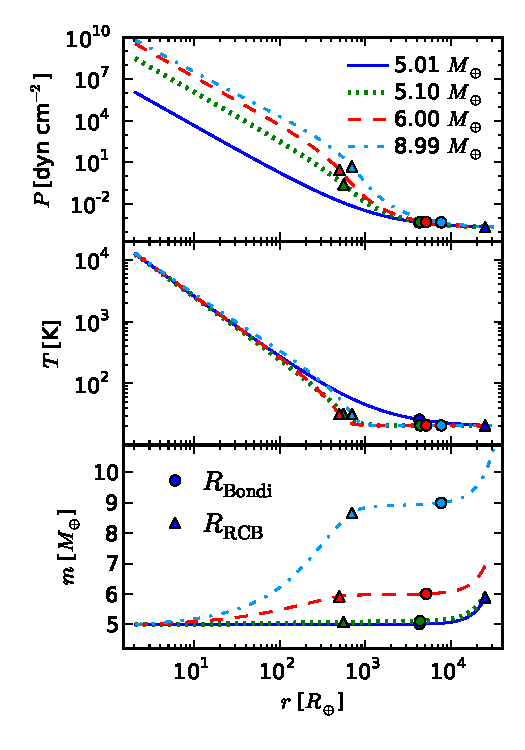
\includegraphics[width=0.5\textwidth]{figures/PTm_profiles_v2_smallM.pdf}
%\vspace{-0.5in}
\caption{Radial profiles of atmospheric pressure, temperature and enclosed mass (core included) for a $5 M_{\oplus}$ core at $60$ AU.   Solid, dotted, dashed and dot-dashed lines correspond to solutions with total mass (core and atmosphere) of $5.01 M_{\oplus}$, $5.10 M_{\oplus}$, $6.00 M_{\oplus}$ and $8.99 M_{\oplus}$, respectively (see text for significance of these masses).  Circles and triangles mark the locations of the Bondi radii and of the radiative-convective boundaries, respectively.  The radial profiles extend from the core to the Hill radius.} %  (See text for a description of evolution to yet higher masses.) 
\label{fig:profiles}
\end{figure}


\subsection{Atmospheric Structure}
\label{sec:profiles}
Figure \ref{fig:profiles} shows radial profiles at different stages of atmospheric growth around a $5 M_{\oplus}$ core at $60$ AU.  Quoted mass values include the core plus atmosphere within the smaller of $\RB$ or $\RH$, which for these cases is $\RB$.  The 8.99 $M_{\oplus}$ solution is the mass 
that satisfies our runaway growth criteria (described in \S\ref{sec:timeev}). % we can reach in our evolutionary sequence, as we explain further in \S\ref{sec:endoftime}.

The lowest mass atmosphere -- which we take as our initial state -- is fully convective and shares the disk's entropy.  In \Fig{fig:profiles} this state is the 5.01 $M_{\oplus}$ solution with no radiative zone.

Cooling and contraction allow the atmosphere to accrete more gas.  In the convective zones, higher mass solutions have lower entropy and higher pressures.  A radiative zone emerges to connect the lower entropy interior to the higher entropy disk.  \Fig{fig:profiles} shows that this radiative zone is already fairly deep in the 5.10 $M_\oplus$ solution. 
 
The atmospheric structure is well approximated by our non-self-gravitating, analytic solutions.  Deep in convective zones, thermal energy is a fixed fraction of the gravitational potential energy, giving $T \propto r^{-1}$ and $P\propto r^{-1/\delad}$  as in \Eq{eq:deep}.  This behavior is seen in \Fig{fig:profiles} for $r\ll R\cb$. Near the core, \Eq{eq:Tconvdeep} gives the core temperature, $T\co= G M\co / (C_{\rm P} R\co)$, unaffected by  the overlying atmosphere mass which does not contribute to the gravitational potential.  Closer to the RCB, self-gravity is no longer negligible, particularly for large envelope masses. Instead, these high mass solutions show a slightly flatter profile in $T$ and also in $P \propto T^{1/\delad}$, as explained by \Eq{eq:TPsg}.

In agreement with \Eq{eq:cb2}, the radiative zones remain nearly isothermal, even for the higher masses.  Consequently, the pressure increases nearly exponentially with depth.  


\subsection{Time Evolution}\label{sec:timeev}

\begin{figure}[tb]
\centering
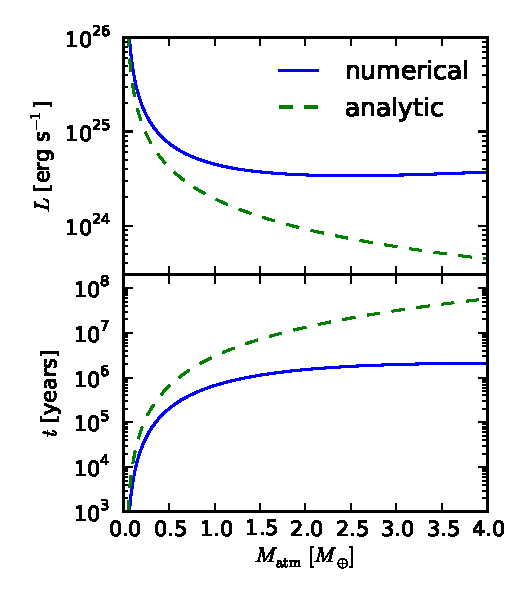
\includegraphics[width=0.5\textwidth]{figures/Lt_profiles_v2.pdf}
%\vspace{-0.5in}
\caption{Evolution of the luminosity and elapsed time during atmospheric growth around a $5 M_{\oplus}$ core at $60$ AU.  The luminosity is initially high, then decreases as the atmosphere grows in mass and the radiative zone becomes optically thicker.  Due to the neglect of self-gravity, the analytic model (\emph{dashed curve}) gives luminosities that are too low and evolution times that are too long.}
\label{fig:Ltplot}
\end{figure}

The cooling model of \S\ref{sec:twolayer} is used to connect solutions with different atmospheric masses into an evolutionary sequence.  \Fig{fig:Ltplot} shows the luminosity evolution and the elapsed time as a function of atmospheric mass for the same parameters as in \Fig{fig:profiles}.

During the early stages of atmospheric growth, the luminosity drops sharply.  This behavior is seen in both the full numerical solutions and the analytic model.  With increasing atmospheric mass, the pressure depth of the RCB increases, along with the optical depth ($\propto \kappa P\cb)$.  Consequently, the radiative luminosity decreases.  This behavior is described in \Eqs{eq:crit}{eq:Lcb}.

At later stages of evolution, the numerical model in \Fig{fig:Ltplot} shows a flat luminosity with increasing mass and also time (not shown).  By contrast, the non-self-gravitating analytic model gives a luminosity that continues to drop as the atmosphere becomes more massive.  To understand this difference, consider the scaling of \Eq{eq:Lcb}, $L\cb \propto M\cb T\cb^4/ (\kappa\cb  P\cb)$, which holds in both cases.   Accounting for the higher enclosed mass in the self-gravitating model gives a somewhat higher luminosity, as desired.  However, the main effect is that \Eq{eq:crit} -- which describes a nearly linear relation between atmospheric mass and RCB pressure --  breaks down for self-gravitating solutions.  This behavior can be seen in the top panel of \Fig{fig:profiles} where the $P\cb$ increases significantly from 5.10 to 6.0 $M_\oplus$, but only increases relatively modestly with further growth to 8.99 $M_\oplus$.   In the higher mass solutions, the relatively low $P\cb$ values (and thus the relatively high luminosities) require an outward shift in $R\cb$, as shown in \Fig{fig:profiles}. This shift does not occur in the analytic solution, where $R\cb$ continually decreases with atmospheric mass (cf. Equations \ref{eq:PcbRcb} and \ref{eq:crit}).

The accelerated growth in the numerical model, as shown in the bottom panel of \Fig{fig:Ltplot}, is also a direct result of the higher cooling luminosities with self-gravity included.  Even when $M_{\rm atm} / M\co$ is only few percent, i.e.\ well before the crossover mass, the effect of self-gravity is  quite evident.  Closer to the star, the effects of self-gravity are not as strong for low atmosphere masses.  Nevertheless, all our models show that self-gravity noticeably accelerates growth for $M_{\rm atm} > 0.1 M\co$.

In \Fig{fig:LtvsMopacity}, our standard dust opacity, \Eq{eq:opacitylaw}, is reduced by factors of 10 and 100.  Lower opacities result in higher luminosities and faster evolution.  Our model thus confirms a well-established result \citep{HubBod05}.  While clearly an important effect, atmospheric dust opacities are difficult to robustly predict. Ablation of infalling solids is a dust source.  Sinks include the sequestration of solids in the core and dust settling through the radiative zone.  Grain growth both reduces dust opacities per unit mass and favors settling.  Our scenario of negligible ongoing particle accretion tends to favor low dust opacities.   To be conservative, however, our reference case considers full Solar abundances. The effect of opacity reduction on the critical core mass is described in \S\ref{sec:critical}. 

\begin{figure}[tb]
\centering
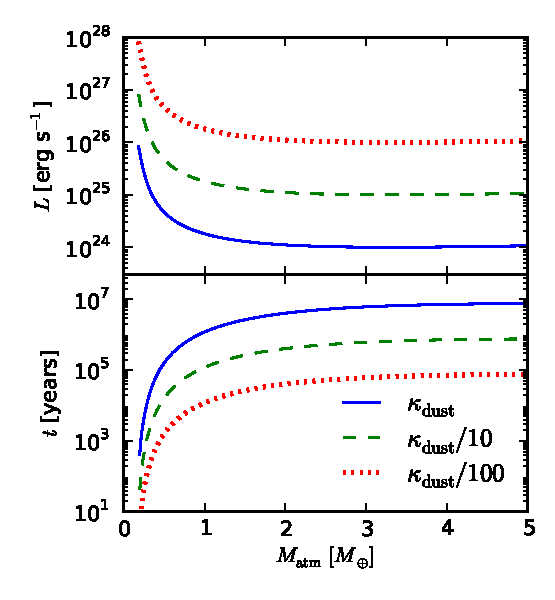
\includegraphics[width=0.5\textwidth]{figures/opacity_effect.pdf}
%\vspace{-0.5in}
\caption{The effect of dust abundance on atmospheric evolution.   Reducing dust opacities by factors of 10 and 100 from standard Solar abundances gives higher luminosities and faster atmospheric growth.  Plotted quantities are similar to \Fig{fig:Ltplot}, but for a $5 M_{\oplus}$ core at 10 AU. }  %The actual magnitude of dust opacities is difficult to robustly predict.}
\label{fig:LtvsMopacity}
\end{figure}

\Fig{fig:growthtime} plots the evolution of the atmospheric growth timescale, $M_{\rm atm}/\dot{M}$,  around a $5 M_{\oplus}$ core at several locations in our reference disk model.  This instantaneous growth time shows clearly that the atmosphere spends the bulk of its time growing though intermediate atmospheric masses, $\sim 1 -3$ $M_\oplus$ in this case.  Growth times are short both early -- when the radiative zone is transparent -- and late -- when self-gravity accelerates growth.  

The fact that growth times have a well defined maximum is a characteristic of accelerating growth.  Unlike our analytic model, which must assume that runaway growth begins near the crossover mass, our numerical model allows us to measure when runaway accretion starts.  Runaway growth does not begin at a universal value of $M_{\rm atm}/M\co$.  Further from the star, runaway growth begins at smaller $M_{\rm atm}/M\co$, as \Fig{fig:growthtime} shows.  \Fig{fig:tvsM} (described in the next section) shows how the onset of runaway growth depends on core mass. 

We quantify the runaway growth timescale, $t_{\rm run}$, as the time when $M_{\rm atm}/\dot{M}$ drops to 10\% of its maximum value.  The choice of 10\% is arbitrary; the precise threshold chosen is relatively unimportant because growth continues to accelerate.

%The onset of runaway growth at high masses is also evident in \Figs{fig:Ltplot}{fig:LtvsMopacity} (bottom panels) as the flattening of the $t$ vs.\ $M_{\rm atm}$ curve.  

\begin{figure}[tb]
\centering
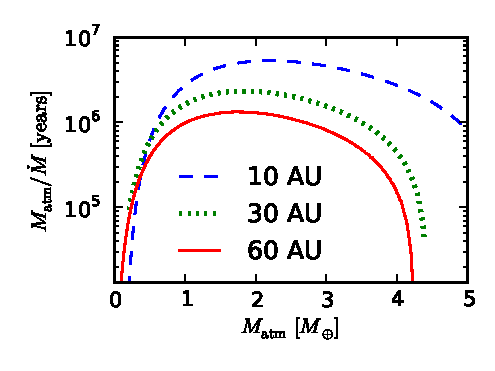
\includegraphics[width=0.5\textwidth]{figures/Mt_profile_temp.pdf}
%\vspace{-0.5in}
\caption{Evolution of the atmospheric growth timescale with mass around a $5 M_{\oplus}$ solid core  located at 10, 30 or 60 AU, for standard Solar opacities.  Growth is slowest for $M_{\mathrm{atm}} \sim 1 - 3 M_{\oplus}$, i.e.\ before the crossover mass at $M_{\rm atm} = M\co$.}
\label{fig:growthtime}
\end{figure}

\subsection{Validity of the Two-Layer Cooling Model}
\label{sec:endoftime}

We examine the  validity of our cooling model by comparing our model luminosity to the neglected luminosity, $L_{\rm negl}$,  that a more detailed model would generate in the radiative zone.  We compute $L_{\rm negl}$ from the entropy difference between successive radiative zone solutions.  We then integrate the energy equation, $\p L / \p m = - T \p S/ \p t$, over the average depth of the radiative zone.\footnote{While useful as a diagnostic, the neglected luminosity cannot reliably correct the global cooling model because the effects of $L_{\rm negl}$ on the structure of the radiative zone are still ignored.}

 \Fig{fig:coolingterms} shows that the neglected luminosity is indeed negligible during the early stages of evolution.  However, $L_{\rm negl}$ exceeds the model luminosity, $L$, at high masses, $M_{\rm atm} > 3 M_\oplus$ in this case.  Our cooling model is thus inaccurate at higher masses.  However, the model remains reasonably accurate up to the beginning stages of runaway growth, which is sufficient for our purposes of widely exploring parameter space and exploring trends.
 
The individual terms in the global cooling model of \Eq{eq:coolingglobal}, evaluated at the RCB, are also plotted in \Fig{fig:coolingterms}.  At low masses, the change in energy, $- \dot{E}$, makes the dominant contribution to luminosity.  As the mass increases, the surface terms become more significant, led by the accretion energy.  However, the surface terms are everywhere smaller than $L_{\rm negl}$.  Thus wherever our model is accurate -- including the crucial early phases of growth -- surface terms are a minor correction.  The neglect of surface terms in the analytic model is thus not a serious omission.

%At even higher masses than shown in \Fig{fig:coolingterms}, our cooling model breaks down.  Mathematically, the breakdown manifests as a negative time step (due to an increase in internal entropy) when advancing to a higher atmospheric mass.  This unphysical result has no deep significance, as the neglected luminosity overwhelms the model luminosity by this point.    Effectively the model is telling us when to ignore it.  Our results are unaffected by the breakdown, which occurs comfortably after $t_{\rm run}$, our threshold for runaway growth.  

 
\begin{figure}[tb]
\centering
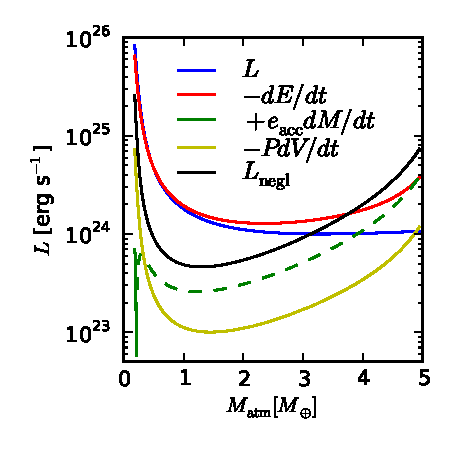
\includegraphics[width=0.5\textwidth]{figures/cooling_a10_Mc5_rcb.pdf}
%\vspace{-0.5in}
\caption{Individual terms in the atmospheric cooling model of \Eq{eq:coolingglobal}, for a $5 M_\oplus$ core at 10 AU.  The dashed curve for accretion energy indicates a negative contribution.  All quantities are evaluated at the RCB, except for $L_{\rm negl}$, the extra luminosity that would have been generated in the radiative zone, but is neglected in our model. The neglected luminosity is a small correction to the model luminosity $L$ for $M_{\rm atm} \lesssim 3 M_{\oplus}$.   Since these low masses dominate growth times, our model is roughly accurate.}
\label{fig:coolingterms}
\end{figure}



\section{Results for Giant Planet Formation}
\label{sec:critical}

%We now use our structure and evolution models to calculate the necessary conditions for gas giant formation by core accretion.   
We now use our structure and evolution models to estimate the timescales and minimum core masses for giant planet formation for a range of disk conditions and other model parameters.  Our results for atmosphere growth times -- the time for a core of fixed mass to undergo runaway gas accretion -- are presented in \S\ref{sec:tcross}.  Section \ref{sec:critcore} gives our results for critical core masses, the minimum values that trigger runaway atmospheric growth within a plausible disk lifetime, here 3 Myr.

Our models focus on giant planet formation between 5 and 100 AU, as the outer disk is of particular interest for direct imaging searches.   The growth of atmospheres close to the star is also important, but spherical accretion models (including ours) are less applicable here.  In the inner disk, critical core masses increase, yet lower mass planets start to open gaps and outgrow the disk scale height, see \Eq{eq:Mth}.  These concerns prevent us from applying our model to the inner disk. 


\subsection{Runaway Growth Timescale}
\label{sec:tcross}
The time to undergo atmospheric runaway growth, $t_{\rm run}$, sets a minimum timescale for the formation of giant planets.  Due to the accelerating nature of runaway growth, the precise threshold chosen for $t_{\rm run}$ (explained in \S\ref{sec:timeev}) is of minor significance.

\begin{figure}[tb]
%\centering
\hspace{-.1in}
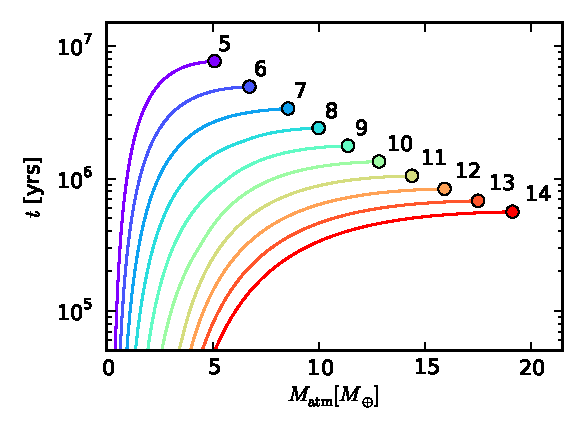
\includegraphics[width=0.5\textwidth]{figures/cumul_coolingtime_vs_Matm_10au_mu235.pdf}
%\vspace{-0.5in}
\caption{Time to grow an atmosphere of mass $M_{\rm{atm}}$ for cores with fixed masses between $5 M_{\oplus}$ and $14 M_{\oplus}$ (as labeled) at $10$ AU in our fiducial disk. Circles mark the runaway growth time, $t_{\rm run}$, which occurs at roughly the crossover mass, $M_{\rm{atm}} = M\co$.  Both the time to reach a fixed atmosphere mass and the runaway growth time are shorter for larger cores. For larger $M\co$, runaway growth commences at higher $M_{\rm atm}/M\co$ values.}
\label{fig:tvsM}
\end{figure}

\begin{figure}[htb]
\centering
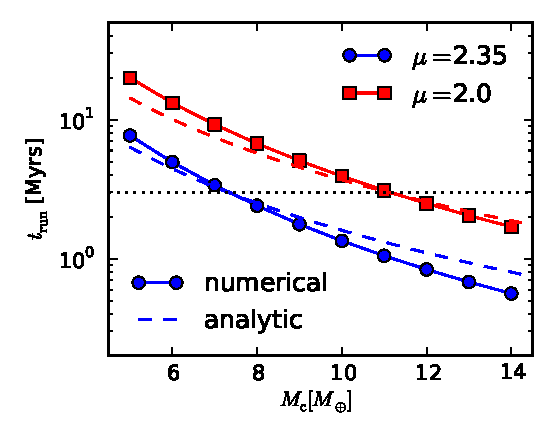
\includegraphics[width=0.48\textwidth]{figures/coolingtime_vs_Mc_10au.pdf}
%\vspace{-0.5in}
\caption{Runaway growth time, $t_{\rm{run}}$, vs.\ core mass at $10$ AU, for two values of the mean molecular weight.  Our numerical model (\emph{solid curves}) is compared to our non-self-gravitating analytic model (\emph{dashed curves}, from Equation \ref{eq:tcoolanf}).  A typical protoplanetary disk life time of $3$ Myr is plotted for comparison. The runaway growth time is larger for a lower mean molecular weight.}
\label{fig:tvsMcomp}
\end{figure}


\subsubsection{Effects of Core Mass}
\label{Mct}

\Fig{fig:tvsM} shows the growth of atmospheric mass with time for several core masses at $10$ AU in our fiducial disk.  Atmospheres grow faster around more massive cores due to stronger gravitational binding.  The endpoint of each curve marks $t_{\rm run}$.   Runaway growth occurs near the crossover mass, when $M_{\rm atm} \sim M\co$, in agreement with previous studies. Lower core masses undergo runaway accretion at fractionally smaller atmosphere masses. %Thus, when compared to the assumption that runaway occurs at a universal $M_{\rm atm}/M\co$ ratio,  effects that lower the critical core mass are amplified by the earlier onset of runaway growth.

\Fig{fig:tvsMcomp} shows how $t_{\rm run}$ varies with core mass, also at 10 AU.  The numerical results are plotted against our non-self-gravitating analytic model, described in \S\ref{sec:coolingan}.  The analytic model reproduces the general decline in $t_{\rm run}$ with core mass.  The numerical model, which includes self-gravity, has a somewhat steeper mass dependence.  A modest correction due to self-gravity is unsurprising, and consistent with the above-mentioned trend in $M_{\rm atm}/M\co$ ratios.  Moreover, in the analytic theory, crucial quantities like $M_{\rm atm}$ and $L$ (both roughly $\propto M\co^3$ near crossover) have non-linear dependence on core mass, offering plenty of opportunity for self-gravitational corrections.

The effect of mean molecular weight is also shown in \Fig{fig:tvsMcomp}.  A lower $\mu$ gives longer growth times, because more cooling is required to compress the atmosphere.  This effect is both well established in core accretion studies \citep{stevenson82} and intuitive since the atmospheric scale height $\propto 1/\mu$ is more extended for lower $\mu$.   Moreover, the Bondi radius decreases as $\RB \propto \mu$, giving a smaller gravitational sphere of influence (and a weaker compression at $\RH$ when that is the more relevant scale).  To see how this affects cooling times, note that the characteristic RCB depth near runaway scales as $P\cb \sim P_{\rm M} \propto \mu^{-4}$ from \Eq{eq:PM}.  Thus $L \propto 1/P\cb \propto \mu^4$ explains the trend of slower cooling for lower $\mu$.
%he larger atmospheric scale height due to a lower $\mu$ also results in a larger pressure depth at the RCB, $P\cb$, and thus a lower $R\cb$, cf. \Eq{eq:PcbRcb}.} 

For $\mu = 2.0$, which represents the idealized case of an H$_2$ atmosphere completely devoid of Helium, $t_{\rm run}$ increases by factors of $\sim 2 - 3$.  Thus fairly drastic changes in atmospheric composition are required for $\mu$ to significantly affect core accretion timescales. In principle, changes in the mean molecular weight of the gas also affect the EOS, including $\delad$, but such effects are not considered here (see \S\ref{sec:EOS}).



\begin{figure*}[tb]
\centering
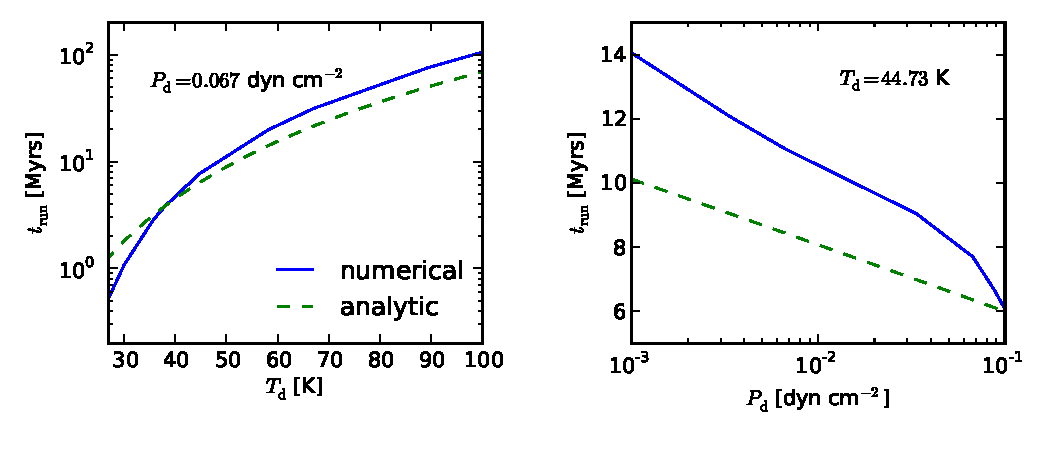
\includegraphics[width=1.\textwidth]{figures/TdPd_effect.pdf}
\vspace{-0.3in}
\caption{Runaway growth time as a function of disk temperature (\emph{left}) and pressure (\emph{right}) around a $M_{\rm c} = 5 M_{\oplus}$ core.   The disk pressure or temperature (\emph{left} or \emph{right}, respectively) are fixed at values for 10 AU in our disk model.   The analytic scalings given by \Eq{eq:tcoolanf} are plotted for comparison, as described in the text.  Gas accretion slows down significantly at higher temperatures, but only speeds up modestly as the disk pressure or density increase.} 
\label{fig:TPeffects}
\end{figure*}


\subsubsection{Effects of Disk Temperature and Pressure}
\label{sec:TPeffects}

\Fig{fig:TPeffects} shows how the runaway accretion time varies with disk temperature, $T\di$, or pressure, $P\di$, holding the other quantity fixed.   The analytic model roughly reproduces the temperature and pressure scalings, again with some discrepancies due mainly to the neglect of self-gravity.  Temperature variations are much more significant than pressure variations (note the difference in logarithmic and linear axes).  Since midplane disk conditions depend only on temperature and pressure in our model,\footnote{See \Eq{eq:diskparam}.  When gap opening is considered in models of later growth stages, the orbital frequency and effective viscosity become relevant as well.} the dominant effect of disk location is temperature.  

The decline in growth times with lower temperatures arises from a balance of competing effects.  The cooling luminosity is inherently smaller at lower temperatures.  Overpowering this effect, the larger Bondi radius and lower dust opacity act to accelerate growth at lower temperatures.

Growth times depend only weakly on, but do fall slightly with, pressure.   This result may be surprising, given that the disk is the source of atmospheric mass and the atmosphere must match onto the disk's density and pressure.  The nearly exponential increase in pressure with depth through the radiative zone explains this effect.  Cooling is largely regulated at the RCB, and a modest change in RCB depth compensates for large variations in disk pressure.

Section \ref{sec:coolingan} shows how these temperature and pressure effects arise in our analytic model.


\begin{figure}[htb]
\centering
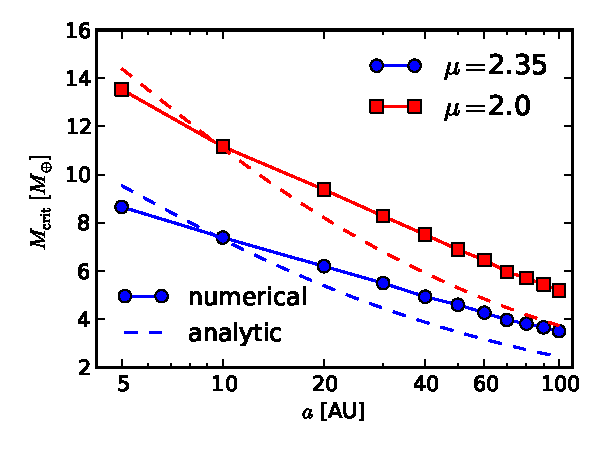
\includegraphics[width=0.5\textwidth]{figures/Mcrit_vs_a_3Myrs_new.pdf}
%\vspace{-0.5in}
\caption{The critical core mass as a function of semimajor axis, for a disk lifetime of $3$ Myrs and two values of the mean molecular weight ($\mu = 2.35$ is for Solar abundances). The decline in $\MC$ with distance is a robust result for standard disk models.  The analytic model, which neglects self-gravity, over-predicts the steepness of the decline.}
\label{fig:Mcvsa}
\end{figure}

\begin{figure}[htb]
\centering
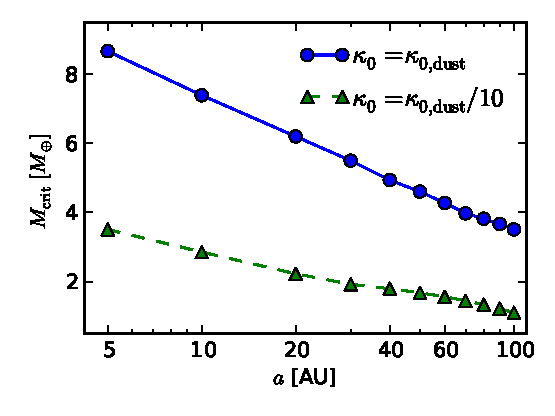
\includegraphics[width=0.5\textwidth]{figures/Mcrit_vs_a_3Myrs_opacity.pdf}
%\vspace{-0.5in}
\caption{Critical core masses vs. distance for standard and reduced (by a factor of ten) dust opacities.  Lower opacities give significantly lower $\MC$ values.  Atmospheric opacity remains a large uncertainty in core accretion models.}
\label{fig:Mcritopacity}
\end{figure}

\subsection{Critical Core Mass}
\label{sec:critcore}

The critical core mass declines with distance from the star, as shown in \Fig{fig:Mcvsa} for our standard disk model.   The main reason for the decline, as explained above, is that atmospheres grow faster at lower temperatures.  The lower densities and pressures in the outer disk have a much smaller effect.  Since the vast majority of disk models have a disk temperature that declines with $a$, our qualitative result is robust.   We also show that higher $\mu$ values give lower values of $\MC$.

The average power-law decline from 1 to 100 AU (not plotted) is $\MC \propto a^{-0.3}$, for both choices of $\mu$.   While not a drastic decline, the ability of distant low mass cores to accrete gas efficiently is significant for the interpretation of direct imaging surveys.  However, our model offers no guarantee of copious giant planets at large distances.  Many histories of solid accretion are possible, and solid cores may grow too slowly to allow the rapid gas accretion that we model.  

Our non-self-gravitating analytic model (dashed curves in \Fig{fig:Mcvsa}) over-predicts the steepness of the decline in $\MC$ with $a$.  This discrepancy is not surprising, as we have shown that self-gravity strongly affects evolution, even before runaway growth begins and the crossover mass is reached.

\Fig{fig:Mcritopacity} shows that reducing the opacity by an order of magnitude significantly reduces $\MC$.  Furthermore, this opacity effect is stronger at larger distances.  The opacity reduction by a factor of 10 lowers $\MC$ at 5 AU by a factor of $\sim$$2.5$ and at 100 AU by a factor of $\sim$$3.5$.  Atmospheric opacity is a dominant uncertainty in core accretion modeling.  However, unless atmospheric opacity varies significantly with disk radius, the general decline in $\MC$ with increasing $a$ should hold.  For our scenario of negligible ongoing planetesimal accretion, it is tempting to think that dust could settle out of the radiative zone, lowering the opacity \citep{podolak03}.  Nonetheless, since opacity near the RCB is a crucial factor, we speculate that convective overshoot may prevent very low opacities.

A larger disk lifetime further reduces $M_{\rm crit}$. Recent studies have shown that gas disks may live up to $\propto$$10-12$ Myr \citep{bell13}. As $M_{\rm crit} \sim t\di^{-3/5}$ (cf. Equation \ref{eq:tcoolan}), a disk lifetime of 10 Myrs decreases the critical core mass by a factor of two.  Of course, some fraction of the disk lifetime must be allocated to the growth and possibly migration of the core.



%\textbf{As the core is assumed to form through accretion of solids, we require that $M_{\rm crit}>M_{\rm isol}$. Since $M_{\rm crit}$ decreases with semi major axis, while $M_{\rm isol}$ increases with $a$ (cf. Equation \ref{eq:Misol}), it is possible that the isolation mass may become larger than the critical core mass at large orbital distances. From \Eq{eq:Misol}, $M_{\rm isol} \approx 1 M_{\oplus}$ at 100 AU, which is smaller than $M_{\rm crit}$ under standard opacity assumptions, but comparable for a reduced opacity (see Figure \ref{fig:Mcritopacity}). A flatter surface density profile (see \S\ref{sec:disk}) may further increase $M_{\rm isol}$. We note, however, that the estimate of \Eq{eq:Misol} assumes an initial uniform dust-to-gas ratio throughout the disk, although the dust-to-gas ratio may be distance dependent. A lower dust-to-gas ratio in the outer disk reduces $M_{\rm isol}$. As stated in \S\ref{sec:scales}, we assume that the isolation mass is always lower than our calculated $M_{\rm crit}$.}


%\textbf{Finally, the mass at which core growth rapidly decreases due to depletion of planetesimals from the core's feeding zone is called the isolation mass. For our fiducial disk model and for an assumed dust-to-gas ratio of 0.01, the isolation mass is given by}
%
%\begin{equation}
%\label{eq:Misol}
%M_{\rm isol} \sim 2 \pi a \times 2 \RH \times \Sigma_{\rm p} \approx 0.2 a_{10}^{3/4} ~ M_{\oplus},
%\end{equation}
%\textbf{where $\Sigma_p$ is the surface density of solids. Since in our regime the core is no longer accreting solids, we require $M_{\rm isol}$ to always be smaller than the core mass at which runaway gas accretion commences, i.e. the critical core mass.}

\subsection{Comparison with Previous Studies}
\label{sec:comp}

We can directly compare our results with other studies of protoplanetary atmospheric growth in the absence of planetesimal accretion, notably those in I00 and PN05.  A major distinguishing feature of our study is that we explore a range of disk conditions, while I00 and PN05 focus on growth at the location of Jupiter, 5.2 AU, in their disk models.  Moreover, both I00 and PN05 solve the full time dependent energy equation and consider more detailed EOSs, in addition to other detailed differences in model parameters.  Despite these differences, the qualitative and quantitative agreement with our study is good.

I00 give an approximate analytic fit to their models' envelope formation time (the equivalent of the runaway accretion time $t_{\rm run}$ in our models), at $a=5.2$ AU, 
\begin{equation}
\label{eq:tauenv}
\tau_{\rm env} \sim 3 \times 10^8 \Big(\frac{M\co}{M_{\oplus}}\Big)^{-2.5} \Big(\frac{\kappa}{1 \text{cm$^2$ s$^{-1}$}}\Big) \,\,\, \text{yr}\, .
\end{equation}
Our model reproduces the linear opacity dependence (see \S\ref{sec:timeev}), even though we use a temperature dependent opacity, \Eq{eq:opacitylaw}, instead of a constant $\kappa$.  Our growth times at 5 AU,
\begin{equation}
\label{eq:trun5au}
t_{\rm run} \sim 5 \times 10^8 \Big(\frac{M\co}{M_{\oplus}}\Big)^{-2.4} \,\,\, \text{yr},
\end{equation} 
agree well with the I00 results, both in magnitude and scaling with core mass.

One goal of our study was to explain the extended luminosity minimum in evolutionary models that characterizes phase 2 in core accretion models, as described in the introduction.  Previous work (see Figure 2 in I00 and Figures 3 and 4 in PN05) shows that this luminosity minimum is an intrinsic feature of atmospheric cooling even in the absence of planetesimal accretion.  We not only reproduce this effect in our simplified model (see \Figs{fig:Ltplot}{fig:LtvsMopacity}), but we also show that self-gravity is the essential ingredient to produce a broad luminosity minimum well before the crossover mass.  

Time-dependent studies that incorporate planetesimal accretion generally find larger formation timescales and critical core masses than those of this work.  This result is expected since additional energy from planetesimal accretion limits the ability of the atmosphere to cool. \citet{pollack96} find an evolutionary time and crossover mass of $\sim$$7.5$ Myrs and $\sim$$16 M_{\oplus}$, respectively, for a MMSN disk model at 5.2 AU and interstellar grain opacity. These values, however, decrease to $\sim$$3$ Myrs and $\sim$$12 M_{\oplus}$ if planetesimal accretion is entirely shut off during the gas accretion phase. The core accretion model of \citet{HubBod05} for Jupiter's formation predicts an evolutionary time of 3.3 Myrs for a $10 M_{\oplus}$ core, for an interstellar opacity, which is also consistent with our result at 5 AU.

A direct comparison with studies that only include planetesimal accretion, and neglect atmospheric cooling, is difficult.  Note, however, that I00 establishes the correspondence between the minimum luminosity in evolutionary models and the minimum planetesimal accretion rate needed in static models, which gives rise to the classical critical core mass of static models \citep{mizuno78, stevenson82}.

In terms of modern static studies, our results complement (and borrow some tools from) R06 and \citet{Raf11}.  These studies consider the disk radius dependence of core accretion for protoplanets that continuously accrete planetesimals.  We show that the limits on core accretion at large radial distance claimed by \cite{Raf11} (and references therein) can be overcome if planetesimal accretion shuts off and the atmosphere is allowed to cool.  Nevertheless, the plausibility of rapid core growth followed by negligible subsequent solid accretion admittedly remains uncertain, as discussed in more detail in \S\ref{sec:conclusions}.


\section{Neglected Effects}\label{sec:neglected}
Since one goal of this paper was to obtain a detailed understanding of atmospheric evolution with a simple model, we have necessarily ignored   effects of potential significance.  We briefly address the most important of these and note that a followup work, Piso, Youdin \& Murray-Clay (in prep., hereafter Paper II), will extend our current models to address some of these effects.

\subsection{Hydrodynamic Effects}\label{sec:hydro}
The neglect of hydrodynamical effects in our model is best discussed in terms of the thermal mass, $M_{\rm th}$, and the length scales introduced in \S\ref{sec:scales}.  In the low mass regime, $M\pla < M_{\rm th}/ \sqrt{3}$, where $\RB < \RH$, we assume that hydrostatic balance holds out to the outer boundary at $\RH$.   In this low mass regime, \citet{Orm13} calculated the 2D (radial and azimuthal) flow patterns driven by stellar tides and disk headwinds.     On scales $\gtrsim \RB$ the flows no longer circulate the planet: they belong to the disk.  While the density structure still appears roughly spherical and hydrostatic, these flows could affect the planet's cooling.  We expect such effects to be weak, as heat losses at greater depths dominate planetary cooling, but more study is needed, especially in 3D.

 %Nevertheless, the density structure outside $\RB$ remains spherically symmetric and hydrostatic.  

At higher masses, non-hydrostatic effects become more severe.  At $M\pla \gtrsim M_{\rm th}$ planets can open significant gaps \citep{zhu13}.  At yet higher masses accretion instabilities could occur \citep{AylBat12}.  However, in this high mass regime, the spherically symmetric approximation has already broken down. 

Thus by restricting our attention to low masses, neglected hydrodynamic effects should be minor.   Moreover, since $M_{\rm th} \propto a^{6/7}$ increases with disk radius, spherical hydrostatic models like ours have a greater range of applicability in the outer regions of disks. 


\subsection{Realistic Opacities}\label{sec:op}

The importance of envelope opacity is an established factor in core accretion calculations (e.g., \citealt{stevenson82}, \citealt{ikoma00}, R06), and several studies explore the influence of opacity on the timescales for giant planet formation in detail (e.g., \citealt{HubBod05}). Treating dust (and total) opacities as a power law in temperature is a simplification.  Opacities drop by order unity when ice grains sublimate for $T \gtrsim 150$ K and they drop by orders of magnitude when silicate grains evaporate above $T \gtrsim 1500$ K \citep{semenov03, FerAle05}.  Grain growth and composition also affect opacities. Our scenario of no ongoing accretion of solids may result in a grain-free atmosphere, which could substantially reduce the critical core mass ($\sim$$1M_{\oplus}$ in the case of Jupiter, \citealt{hori10}). Paper II explores more realistic opacity laws. 

For this work, we justify a simplified dust opacity by the cool temperatures of both the outer disk and our nearly isothermal radiative zones (see \S\ref{sec:profiles}).  While  convective interiors get significantly hotter than 1500 K, opacity does not affect the structure of adiabatic convecting regions.   A possible caveat is the existence of  radiative zones sandwiched inside the convection interior.  Such ``radiative windows" arise if the opacity drop from ice and metal grain sublimation occurs at sufficiently low pressures.  Our two-layer model ignores this possibility, but radiative windows are known to exist in hot Jupiter models \citep{burrows97, ab06} and have been seen in some core accretion models (Lissauer, personal communication).  The role of radiative windows in core accretion models remains to be explored in detail.


\subsection{Equation of State}
\label{sec:EOS}
 
Our model uses an ideal gas law and a polytropic EOS, given by \Eq{eq:idealEOS}.  However, non-ideal effects can affect atmospheric structure and evolution.  In the lower atmosphere, H$_2$ can partially dissociate at high temperatures.  In the upper atmosphere, H$_2$ rotational levels can become depopulated at lower temeratures.   Paper II uses the \citet{saumon95} EOS, with extensions to lower pressures and temperatures as needed, to explore these effects.

\subsection{Core growth}
\label{sec:placc}

Our model purposefully neglects the accretion of solids to study the fastest rates of gas accretion.  Our $\MC$ values thus differ from the $\MC$ values in static models, such as R06.  For similar parameters, we generally obtain lower $\MC$ values than R06 because our atmospheres are not heated by ongoing planetesimal accretion.  Paper II presents a quantitative comparison.



%For giant planet formation to occur with a core mass close to our $M_{\rm crit}$, \textit{in-situ} formation of the core requires $M_{\rm crit}$ to be smaller than the isolation mass, $M_{\rm iso}$. }

%\textbf{As the core is assumed to form through accretion of solids, we require that $M_{\rm crit}>M_{\rm isol}$. Since $M_{\rm crit}$ decreases with semi major axis, while $M_{\rm isol}$ increases with $a$ (cf. Equation \ref{eq:Misol}), it is possible that the isolation mass may become larger than the critical core mass at large orbital distances. From \Eq{eq:Misol}, $M_{\rm isol} \approx 1 M_{\oplus}$ at 100 AU, which is smaller than $M_{\rm crit}$ under standard opacity assumptions, but comparable for a reduced opacity (see Figure \ref{fig:Mcritopacity}). A flatter surface density profile (see \S\ref{sec:disk}) may further increase $M_{\rm isol}$. We note, however, that the estimate of \Eq{eq:Misol} assumes an initial uniform dust-to-gas ratio throughout the disk, although the dust-to-gas ratio may be distance dependent. A lower dust-to-gas ratio in the outer disk reduces $M_{\rm isol}$. As stated in \S\ref{sec:scales}, we assume that the isolation mass is always lower than our calculated $M_{\rm crit}$.}

At low planetesimal accretion rates, $\dot{M}\co$, a static model could formally give lower $\MC$ values than our evolutionary calculations.  R06 shows that $\MC \propto \dot{M}\co^{3/5}$ in static models.  The underlying assumption of static models, a negligibly short KH contraction time, fails whenever static models give a lower $\MC$.  Thus our results give a firm lower limit on $\MC$ which complement the results of static models with planetesimal accretion.

\section{Summary} \label{sec:conclusions}

We study the formation of giant planets by the core accretion mechanism.  Our models start with a solid core that is embedded in a gas disk and no longer accreting solids.  We determine -- as a function of disk location, core mass, and the atmosphere's mean molecular weight and opacity -- whether runaway atmospheric growth can occur within a typical disk lifetime of 3 Myr.  By neglecting the accretion luminosity of planetesimals and smaller solids, we obtain the fastest allowed rate of gas accretion.  

We address core accretion in the outer disk, as it is relevant to direct imaging surveys.  Our model approximations, including spherical accretion and low mass radiative exteriors with opacities dominated by dust, are tuned to conditions in the outer disk.   Our main findings are as follows:

\begin{enumerate}
\item The minimum or critical core mass, $\MC$, for giant planet formation declines with stellocentric distance in standard protoplanetary disk models.  For our reference case, the critical mass is $\sim$$8.5 M_{\oplus}$ at $a = 5$ AU, decreasing to $\sim$$3.5 M_{\oplus}$ at $a =100$ AU.  This decline roughly follows $\MC \propto a^{-0.3}$.

\item The drop in disk temperature with radial distance explains the decrease in critical core masses.  The lower pressures and densities in the outer disk only weakly suppress atmospheric growth.

\item Reducing dust opacities by a factor of 10 reduces critical core masses by a factor of $\sim$$3$.  This reduction is somewhat stronger (weaker) at larger (smaller) separations from the star.

\item A larger mean molecular weight reduces critical core masses, in agreement with \citet{HorIko11}.  If enrichment in heavy elements correlates with increased dust opacity, then the stronger opacity effect will dominate, increasing $\MC$.

\item Runaway growth begins roughly at the crossover mass, when atmosphere and core masses are equal, $M_{\rm atm} \sim M\co$, in agreement with previous work \citep{pollack96}.  Further from the star, runaway growth begins at smaller $M_{\rm atm} / M\co$ ratios.  For larger core masses, runaway growth begins at larger values of $M_{\rm atm} / M\co$.

\item Self-gravity affects atmospheric evolution before crossover.  Significant self-gravitational corrections appear when the atmosphere is only $\sim$$10 \%$ as massive as the core.

\end{enumerate}

Rapid gas accretion onto low mass cores could explain the origin of distant directly imaged giant planets \citep{marois08, lagrange10}.  However, our model does not address the details of how solid cores grow, as many possibilities exist and many uncertainties remain. %\textbf{Our brief treatment of core formation is purposeful, as there are large uncertainties in both planetesimal formation and the subsequent processes of core growth, particularly at large orbital distances. Core formation in the outer disk is challenging due to large dynamical times, and cores are unlikely to reach critical masses at $\gtrsim 40-50$ AU under classic core accretion scenarios \citep{Raf11}. However, modern models of aerodynamic pebble accretion (\citealt{ormel10}; \citealt{lambrechts12}) can give faster growth. Moreover, cores can form closer to the star, then migrate or be scattered outwards by other giants in the system \citep{ida13}.} 
For a giant planet to form with a core near the minimum masses we derive, core growth must  first be rapid and then slow significantly, as in phases 1 and 2, respectively, of \cite{pollack96}.

Initial core growth must be fast, compared to the disk lifetime, to get a sufficiently massive core.  Such rapid core growth is possible in a variety of scenarios, including the fastest gas-free planetesimal accretion rates \citep{dones93} and -- probably more relevantly for gas rich disks --  the aerodynamic accretion of mm-m sized ``pebbles" and ``boulders" in gas disks \citep{ormel10, lambrechts12}.  Moreover, cores could form rapidly closer to the star, then migrate or be scattered outwards by already formed giants \citep{ida13}. 
 
A stronger constraint is that core growth subsequently slow severely, to allow the atmosphere to cool and contract.  To be more quantitative, the minimum cooling luminosity in \Fig{fig:Ltplot}, $L\approx 3.5 \times 10^{24}\;\mathrm{erg s}^{-1}$, could be cancelled by low levels of heating from solid accretion.   A core mass doubling timescale of $\sim$$400$ Myr, or faster, would thus provide enough heating to stall atmospheric cooling and growth.   An additional concern is that isolation masses tend to grow with disk radius, as $M_{\rm iso} \propto \varSigma_{\rm p}^{3/2} a^2 \propto a^{3/4}$ under the approximation that the surface density of accreted planetesimals ($\varSigma_{\rm p}$) scales with the gas \citep{youdin13}.   While this behavior is nominally inconsistent with final core masses that decline with distance, the predictive power of the isolation mass is imperfect.   For starters, the efficiency of planetesimal formation remains uncertain.  Moreover, the locality of core growth, which underlies the isolation mass, disappears when accreted solids drift and/or cores migrate significantly. 
  
Thus while our calculations show that low mass cores can grow into gas giants in the outer disk, ongoing solid accretion could prevent significant atmospheric growth.  In the Solar System, the ice giants Uranus and Neptune,  with core (here ice and rock) masses of $\sim 13 -15$ M$_\oplus$, argue for the latter possibility.  Ongoing exoplanet imaging surveys and their successors \citep{hinz12, macintosh12, close14} will help discriminate among the various planet formation pathways in the outskirts of protoplanetary disks.




% For an example of a full page figure, see Fig.~\ref{fig:myFullPageFigure}.


\begin{savequote}[75mm]
This is some random quote to start off the chapter.
\qauthor{Firstname lastname}
\end{savequote}

\chapter{The title of chapter two}

\newthought{Lorem ipsum dolor sit amet}, consectetuer adipiscing elit. Morbi commodo, ipsum sed pharetra gravida, orci magna rhoncus neque, id pulvinar odio lorem non turpis. Nullam sit amet enim. Suspendisse id velit vitae ligula volutpat condimentum. Aliquam erat volutpat. Sed quis velit. Nulla facilisi. Nulla libero. Vivamus pharetra posuere sapien. Nam consectetuer. Sed aliquam, nunc eget euismod ullamcorper, lectus nunc ullamcorper orci, fermentum bibendum enim nibh eget ipsum. Donec porttitor ligula eu dolor. Maecenas vitae nulla consequat libero cursus venenatis. Nam magna enim, accumsan eu, blandit sed, blandit a, eros.

Quisque facilisis erat a dui. Nam malesuada ornare dolor. Cras gravida, diam sit amet rhoncus ornare, erat elit consectetuer erat, id egestas pede nibh eget odio. Proin tincidunt, velit vel porta elementum, magna diam molestie sapien, non aliquet massa pede eu diam. Aliquam iaculis. Fusce et ipsum et nulla tristique facilisis. Donec eget sem sit amet ligula viverra gravida. Etiam vehicula urna vel turpis. Suspendisse sagittis ante a urna. Morbi a est quis orci consequat rutrum. Nullam egestas feugiat felis. Integer adipiscing semper ligula. Nunc molestie, nisl sit amet cursus convallis, sapien lectus pretium metus, vitae pretium enim wisi id lectus. Donec vestibulum. Etiam vel nibh. Nulla facilisi. Mauris pharetra. Donec augue. Fusce ultrices, neque id dignissim ultrices, tellus mauris dictum elit, vel lacinia enim metus eu nunc.

Proin at eros non eros adipiscing mollis. Donec semper turpis sed diam. Sed consequat ligula nec tortor. Integer eget sem. Ut vitae enim eu est vehicula gravida. Morbi ipsum ipsum, porta nec, tempor id, auctor vitae, purus. Pellentesque neque. Nulla luctus erat vitae libero. Integer nec enim. Phasellus aliquam enim et tortor. Quisque aliquet, quam elementum condimentum feugiat, tellus odio consectetuer wisi, vel nonummy sem neque in elit. Curabitur eleifend wisi iaculis ipsum. Pellentesque habitant morbi tristique senectus et netus et malesuada fames ac turpis egestas. In non velit non ligula laoreet ultrices. Praesent ultricies facilisis nisl. Vivamus luctus elit sit amet mi. Phasellus pellentesque, erat eget elementum volutpat, dolor nisl porta neque, vitae sodales ipsum nibh in ligula. Maecenas mattis pulvinar diam. Curabitur sed leo.

Nulla facilisi. In vel sem. Morbi id urna in diam dignissim feugiat. Proin molestie tortor eu velit. Aliquam erat volutpat. Nullam ultrices, diam tempus vulputate egestas, eros pede varius leo, sed imperdiet lectus est ornare odio. Lorem ipsum dolor sit amet, consectetuer adipiscing elit. Proin consectetuer velit in dui. Phasellus wisi purus, interdum vitae, rutrum accumsan, viverra in, velit. Sed enim risus, congue non, tristique in, commodo eu, metus. Aenean tortor mi, imperdiet id, gravida eu, posuere eu, felis. Mauris sollicitudin, turpis in hendrerit sodales, lectus ipsum pellentesque ligula, sit amet scelerisque urna nibh ut arcu. Aliquam in lacus. Vestibulum ante ipsum primis in faucibus orci luctus et ultrices posuere cubilia Curae; Nulla placerat aliquam wisi. Mauris viverra odio. Quisque fermentum pulvinar odio. Proin posuere est vitae ligula. Etiam euismod. Cras a eros.

Nunc auctor bibendum eros. Maecenas porta accumsan mauris. Etiam enim enim, elementum sed, bibendum quis, rhoncus non, metus. Fusce neque dolor, adipiscing sed, consectetuer et, lacinia sit amet, quam. Suspendisse wisi quam, consectetuer in, blandit sed, suscipit eu, eros. Etiam ligula enim, tempor ut, blandit nec, mollis eu, lectus. Nam cursus. Vivamus iaculis. Aenean risus purus, pharetra in, blandit quis, gravida a, turpis. Donec nisl. Aenean eget mi. Fusce mattis est id diam. Phasellus faucibus interdum sapien. Duis quis nunc. Sed enim.

Pellentesque vel dui sed orci faucibus iaculis. Suspendisse dictum magna id purus tincidunt rutrum. Nulla congue. Vivamus sit amet lorem posuere dui vulputate ornare. Phasellus mattis sollicitudin ligula. Duis dignissim felis et urna. Integer adipiscing congue metus. Nam pede. Etiam non wisi. Sed accumsan dolor ac augue. Pellentesque eget lectus. Aliquam nec dolor nec tellus ornare venenatis. Nullam blandit placerat sem. Curabitur quis ipsum. Mauris nisl tellus, aliquet eu, suscipit eu, ullamcorper quis, magna. Mauris elementum, pede at sodales vestibulum, nulla tortor congue massa, quis pellentesque odio dui id est. Cras faucibus augue.

Suspendisse vestibulum dignissim quam. Integer vel augue. Phasellus nulla purus, interdum ac, venenatis non, varius rutrum, leo. Pellentesque habitant morbi tristique senectus et netus et malesuada fames ac turpis egestas. Duis a eros. Class aptent taciti sociosqu ad litora torquent per conubia nostra, per inceptos hymenaeos. Fusce magna mi, porttitor quis, convallis eget, sodales ac, urna. Phasellus luctus venenatis magna. Vivamus eget lacus. Nunc tincidunt convallis tortor. Duis eros mi, dictum vel, fringilla sit amet, fermentum id, sem. Phasellus nunc enim, faucibus ut, laoreet in, consequat id, metus. Vivamus dignissim. Cras lobortis tempor velit. Phasellus nec diam ac nisl lacinia tristique. Nullam nec metus id mi dictum dignissim. Nullam quis wisi non sem lobortis condimentum. Phasellus pulvinar, nulla non aliquam eleifend, tortor wisi scelerisque felis, in sollicitudin arcu ante lacinia leo.

Pellentesque habitant morbi tristique senectus et netus et malesuada fames ac turpis egestas. Vestibulum tortor quam, feugiat vitae, ultricies eget, tempor sit amet, ante. Donec eu libero sit amet quam egestas semper. Aenean ultricies mi vitae est. Mauris placerat eleifend leo. Quisque sit amet est et sapien ullamcorper pharetra. Vestibulum erat wisi, condimentum sed, commodo vitae, ornare sit amet, wisi. Aenean fermentum, elit eget tincidunt condimentum, eros ipsum rutrum orci, sagittis tempus lacus enim ac dui. Donec non enim in turpis pulvinar facilisis. Ut felis.

Cras sed ante. Phasellus in massa. Curabitur dolor eros, gravida et, hendrerit ac, cursus non, massa. Aliquam lorem. In hac habitasse platea dictumst. Cras eu mauris. Quisque lacus. Donec ipsum. Nullam vitae sem at nunc pharetra ultricies. Vivamus elit eros, ullamcorper a, adipiscing sit amet, porttitor ut, nibh. Maecenas adipiscing mollis massa. Nunc ut dui eget nulla venenatis aliquet. Sed luctus posuere justo. Cras vehicula varius turpis. Vivamus eros metus, tristique sit amet, molestie dignissim, malesuada et, urna.

Cras dictum. Maecenas ut turpis. In vitae erat ac orci dignissim eleifend. Nunc quis justo. Sed vel ipsum in purus tincidunt pharetra. Sed pulvinar, felis id consectetuer malesuada, enim nisl mattis elit, a facilisis tortor nibh quis leo. Sed augue lacus, pretium vitae, molestie eget, rhoncus quis, elit. Donec in augue. Fusce orci wisi, ornare id, mollis vel, lacinia vel, massa.

%\begin{savequote}[75mm]
%Nulla facilisi. In vel sem. Morbi id urna in diam dignissim feugiat. Proin molestie tortor eu velit. Aliquam erat volutpat. Nullam ultrices, diam tempus vulputate egestas, eros pede varius leo.
%\qauthor{Quoteauthor Lastname}
%\end{savequote}

\chapter{C/O and Snowline Locations in Protoplanetary Disks: The Effect of Radial Drift and Viscous Gas Accretion}

\section*{abstract}
%The C/O ratio is an important signature of giant planet atmospheric composition and disk chemistry. 
The C/O ratio is a defining feature of both gas giant atmospheric and protoplanetary disk chemistry. In disks, the C/O ratio is regulated by the presence of snowlines of major volatiles at different distances from the central star. We explore the effect of radial drift of solids and viscous gas accretion onto the central star on the snowline locations of the main C and O carriers in a protoplanetary disk, H$_2$O, CO$_2$ and CO, and their consequences for the C/O ratio in gas and dust throughout the disk. We determine the snowline locations for a range of fixed initial particle sizes and disk types. For our fiducial disk model, we find that grains with sizes $\sim$$0.5$ cm $\lesssim s \lesssim$ 7 m for an irradiated disk, and $\sim$$0.001$ cm $\lesssim s \lesssim$ 7 m for an evolving and viscous disk, desorb at a size-dependent location in the disk, which is independent of the particle's initial position. The snowline radius decreases for larger particles, up to sizes of $\sim$7~m. Compared to a static disk, we find that radial drift and gas accretion in a viscous disk move the H$_2$O snowline inwards by up to 40 \%, the CO$_2$ snowline by up to 60 \%, and the CO snowline by up to 50 \%. We thus determine an inner limit on the snowline locations when radial drift and gas accretion are accounted for. 


\section{Introduction}
\label{sec:intro}

%\emgr{Background topics: importance of atmospheric chemistry in providing constraints on the formation of giant planets; C/O ratio as important signature of atmospheric chemistry; C/O ratios observationally determined are different from interstellar --- one explanation is the different abundance in gas and dust form of the main C and O carriers, H$_2$O, CO$_2$ and CO, between their respective snowlines (cite \"Oberg et al. 2011).}

%\emgr{Paragraph 1: introduce the topic, context and its relevance in the big picture. Gas giants are important. The chemical composition of their atmospheres constraints their formation and evolution. Is is therefore important to understand the disk well enough to (1) predict what kind of planet compositions result from planet formation in different parts of the disk, and (2) backtrack the planet formation location based on planet composition.}

The chemical composition of protoplanetary disks affects planet formation efficiencies and the composition of nascent planets.
%[Need explicit statement that gas giants accrete their atmospheres from the nebular gas.] 
Gas giants accrete their envelopes from the nebular gas. As such, planet compositions are tightly linked to the structure and evolution of the protoplanetary disk in which they form. It is thus essential to understand the disk chemistry and dynamics well enough to (1) predict the types of planet compositions that result from planet formation in different parts of the disk, and (2) backtrack the planet formation location based on planet compositions. %[split into two sentences]

%\emgr{Add the rest as outlined above.} \\



%\emgr{Paragraph 2: disks are complex, a lot of dynamical and chemical processes going on. However, we have detections of organic molecules. We have detections of snowlines. We see complex chemistry and many molecules we can study.}

%In recent years, the onset and development of sensitive infrared and (sub)millimeter spectroscopic observations has facilitated the detection of organic molecules in the outer regions of protoplanetary disks (e.g., \citealt{oberg10}, \citealt{oberg11c}, \citealt{oberg11b}). [the molecules relevant for this paper are not organics]
%[Topic sentence on that the most important volatiles are ... based on protostellar and comet abundances.]

The structures of protoplanetary disks are complex, and affected by a multitude of chemical and dynamical processes (see review by \citealt{henning13}). From the chemistry perspective, volatile compounds are particularly important. Their snowline locations determine their relative abundance in gaseous and solid form in the disk,. Based on protostellar and comet abundances, some of the most important volatile molecules are H$_2$O, CO$_2$, CO, N$_2$. Recent observations of protoplanetary disks have provided valuable information about the abundances and snowline locations of some of these compounds. For example, the CO snowline has been detected in the disk around TW Hya \citep{qi13}, as well as in the disk around HD 163296 \citep{mathews13} using line emissions from DCO$^+$. Observations of TW Hya have also revealed a H$_2$O snowline \citep{zhang13}, and more such snowline detections are expected in future ALMA cycles. These observations are currently lacking an interpretive framework that takes into account all important dynamical and chemical processes. Furthermore, such a framework is crucial to connect observed snowline locations to planet formation.

%Of particular importance are volatile compounds, such as H$_2$O, CO$_2$, CO, N$_2$ etc. Recent detections of the snowlines of volatiles (such as the CO snowline, \citealt{qi11}) are significant, since the snowline locations of these molecules determine their relative abundance in gaseous and solid form in the protoplanetary disk, and thus the chemical composition of nascent giant planets. [I think this paragraph belongs further down after you have discussed planets since that is the topic of your intro paragraph above. Also need a bit more meat here. So far a single CO snowline detection and a single H2O snowline detection. More are expected and an interpretive framework is key regardless of the importance for planets.]%Recent detections of the CO snowline in disks (e.g., \citealt{qi11}) provide the framework...

%\emgr{Add part about snowlines, complex chemistry, many molecules.} \\



An important consequence of snowline formations in disks is that disks are expected to present different carbon-to-oxygen (C/O) ratios in the gas and in icy dust mantles at different disk radii. This effect was quantified by  \citet{oberg11}, who considered the fact that the main carries of carbon and oxygen, i.e. H$_2$O, CO$_2$ and CO, have different condensation temperatures. This changes the relative abundance of C and O in gaseous and solid form as a function of the snowline location of the volatiles mentioned above. \citet{oberg11} calculated analytically the C/O ratio in gas in dust as a function of semimajor axis for passive protoplanetary disks and found a gas C/O ratio of order unity between the CO$_2$ and CO snowlines, where oxygen gas is highly depleted. This effect was used to explain claims of detections of superstellar C/O ratios in exoplanet atmospheres (e.g., WASP-12b, \citealt{madhu11}), which however have been unambiguously refuted (\citealt{stevenson14}, \citealt{kreidberg15}).
%Superstellar C/O ratios have also been detected in the atmospheres of gas giants such as WASP-12b \citep{madhu11}.

%Given the tight connection between planet and disk compositions, detections of C/O ratios in exoplanet atmospheres can provide some insight into the relative abundance of C and O in disks. Spectroscopic observations of gas giants such as WASP-12b have found atmospheric C/O ratios close to unity, substantially different from the Solar value of 0.54 \citep{madhu11}. One explanation for this discrepancy was proposed by \citet{oberg11}, who considered the fact that the main carries of carbon and oxygen, i.e. H$_2$O, CO$_2$ and CO, have different condensation temperatures. This changes the relative abundance of C and O in gaseous and solid form as a function of the snowline location of the volatiles mentioned above. \citet{oberg11} calculated analytically the C/O ratio in gas in dust as a function of semimajor axis for passive protoplanetary disks and reproduced a gas C/O ratio of order unity between the CO$_2$ and CO snowlines, where oxygen gas is highly depleted. %[This is not a very natural approach I think, i.e. to use a dicy eco-planet C/O detection to infer something about the disk chemical composition.]

%\emgr{Paragraph 3: let's focus on one (set of) molecules: the C/O ratio. It's an important signature of atmospheric chemistry. While we cannot detect it directly in disks, we have observations in giant planet atmospheres. It's different than stellar. Why? Possible explanation based on snowlines.}

%\emgr{Start with the fact that we can't see C/O in disks directly. Then transition to planet atmospheres and modify the next sentence to follow up logically.} 
%Notably, an important signature of giant planets atmospheric chemistry is the carbon to oxygen (C/O) ratio. 
 
\citet{oberg11} assumed a static disk with no chemical evolution. In reality, dynamical and chemical processes affect the snowline locations and the resulting C/O ratio. Several works have addressed some of these effects. \citet{madhu14} use a steady-state active disk model that includes planetary migration and use the C/O ratio to constrain migration mechanisms. \citet{alidib14} calculate the C/O ratio throughout the disk by incorporating the evolution of solids, i.e. radial drift, sublimation and grain coagulation, as well as the diffusion of volatile vapors. \citet{alidib14} use the 1+1D $\alpha$-disk model of \citet{hughes10}, in which the gas drifts outwards in the disk midplane, and thus small particles that are well-coupled to the gas will also advect outward. Their model assumes a cyclical conversion between H$_2$O or CO dust and vapor: large enough particles that are decoupled from the gas drift inwards and start desorbing. Once their sublimation is complete, back-diffusion moves the H$_2$O or CO vapor ouwards to their respective snowlines, where they instantly condense into mm-sized particles that diffuse outwards with the gas while coagulating into larger particles. Once the grains become large enough to decouple from the gas and drift inwards, the cycle restarts. This ```conveyor belt''' model is based on the pioneering work by \citet{cuzzi04}, and \citet{ciesla06} for the evolution of H$_2$O in a viscous disk. This approach leads \citet{alidib14} to find that the gaseous C/O ratio increases with time inside the H$_2$O snowline, approaching unity at 2 AU after $\sim$$10^4-10^5$ years.  \citet{thiabaud15} consider additional carbon carrier volatile species in their chemical network, such as CH$_4$, and find that the gas C/O ratio may be enriched by up to four times the Solar value in the outer parts of the disk where CH$_4$ and CO are the only gaseous carriers of C and O.  They also include nitrogen carriers such as N$_2$ or NH$_3$, and perform similar calculations for nitrogen. 

%Most studies of the C/O ratio in disks are particularly focused on the inner disk, in order to explain observations of super-stellar C/O ratios in the atmospheres of close-in exoplanets \citep{madhu11}. In addition, the simultaneous inclusion of various dynamical and/or chemical processes makes it difficult to quantify the separate effect of each of these processes on snowline locations and the C/O ratio. %[The preceding paragraph needs to be made clearer. Currently it is not clear what effects these studies have had on our understanding of C/O ratio sin disks and why your study is needed. I.e. why are the processes you focus on the most important ones? Introduce separately papers that deal with C/O and water snowline locations.]
Each of these studies have considered a specific combination of dynamical and chemical effects. One scenario that has not yet been considered is the combination of radial drift and viscous gas accretion in isolation. Studying these two dynamical processes makes it possible to quantify their separate effect on snowline locations and the C/O ratio at various disk radii.

 %In this paper, we focus on these two particular dynamical processes.  %i.e. the radial drift of solids and viscous gas accretion. %We enhance the model of \citet{oberg11} by considering these two additional processes. 
In this paper, we perform a systematic study to understand the detailed qualitative and quantitative effects of radial drift and gas accretion on the H$_2$O, CO$_2$ and CO snowline locations, and the resulting C/O ratio in gas and dust throughout the protoplanetary disk. More importantly, we obtain a limit on how close to the star the snowline locations can be pushed by radial drift and gas accretion.   

%\emgr{Paragraph 4: the static disk model is a great start, but there are additional dynamical and chemical processes to take into account. Several studies have done that in some form or another --- cite Ali-Dib+14, Madhusudhan+14, Thiabaud+15. Briefly discuss their assumptions.} \\

%\emgr{Paragraph 5: finally introduce our goal for this paper: study the dynamical effects such as drift and gas accretion. State our goals: understand the detailed qualitative and quantitative effect of drift and gas accretion on snowline locations, obtain a limit on how far in can the snowlines be pushed, and see how that affects the C/O ratio throughout the disk. State that our specific goals motivate the use of a simplified model (in other words, why what we are doing is different from the studies cited in the previous paragraph). }

%\emgr{This needs some restructuring and additions along the lines discussed above.} In order to obtain more realistic estimates for C/O ratios across protoplanetary disks, dynamical processes and the disk evolving chemistry have to be taken into account. In this paper, we enhance the model of \citet{oberg11} considering two additional dynamic effects: (1) the radial drift of solids throughout the protoplanetary disk, and (2) the viscous accretion of the disk gas onto the host star. Our goal is two-fold: (1) to quantify the effect of radial drift of solids of different sizes on the location and shape of H$_2$O, CO$_2$ and CO snowlines, and (2) to calculate the resulting C/O ratio in gaseous and solid form throughout an actively accreting protoplanetary disk as a function of the grain size distribution and the evolutionary time of the nebula.


%\emgr{Describe goals and approach of this paper, i.e.: study the importance of radial drift on the location of snowlines in protoplanetary disks and how radial drift affects the C/O ratio. Mention that disks are viscously accreting in the early stages of planet formation, hence gas accretion has to be taken into account. The goal of this paper is two-fold: (1) estimate using both numerical models and analytic arguments the range of particle sizes for which radial drift changes snowline location; (2) calculate the C/O ratio for various particle sizes (and possibly a size distribution) and at different times throughout the evolution of the gas disk.}

This paper is organized as follows. In Section \ref{sec:model}, we present our disk, radial drift and desorption models, as well as the timescales relevant to the coupled drift-desorption process. We calculate the H$_2$O, CO$_2$ and CO snowline locations as a function of particle size for an irradiated and an evolving disk in Section \ref{sec:snowlines}, and the resulting C/O ratio throughout the disk in Section \ref{sec:COratio}. In Section \ref{sec:discussion}, we discuss the generality of our results, as well as additional effects on the snowline locations. Finally, we summarize our findings in Section \ref{sec:summary}.

\section{Model Framework} 
\label{sec:model}

We present our protoplanetary disk model for a static, an irradiated, an evolving, and a viscous disk in section \ref{sec:disk}. In section \ref{sec:drift}, we describe our analytic model for the radial drift of solids. We summarize our ice desorption model in section \ref{sec:desorption}. Finally, we discuss the relevant timescales for dynamical effects that affect snowline locations %in the desorption process 
in section \ref{sec:timescales}.

\subsection{Disk Model}
\label{sec:disk}

To understand the separate effects of radial drift, radial movement of gas throughout the disk due to gas accretion, and accretion heating, we use four separate disk models:  \textit{static disk}, which is solely irradiated by the host star and does not take into account gas accretion onto the star or radial drift; \textit{irradiated disk}, which has the same temperature profile as the static disk and does not experience gas accretion or accretional heating, but it takes into account radial drift of solids; \textit{evolving disk}, in which the gas is accreting onto the central star causing the gas surface density to decrease with time, but which does not experience accretion heating; and \textit{viscous disk}, for which the mass flux $\dot{M}$ is constant in time and independent of semimajor axis, and the temperature profile is calculated using both accretional heating and stellar irradiation.

%[Perhaps define your four disk models up here and motivate why you are exploring several different ones, and then go through and describe them in detail. That would save you the slightly awkward Active disk with passive temperature profile.]

\textbf{Static and Irradiated disk.} We adopt a minimum mass solar nebula (MMSN) disk model for a static and and an irradiated disk similar to the prescription of \citet{chiang10}. The gas surface density and midplane temperature are
\begin{subeqnarray}
\label{eq:disk}
\Sigma&=&2000\, (r/\text{AU})^{-1}\,\, \text{g cm}^{-2} \slabel{eq:disksigma}\\
T &=& 120\, (r/\text{AU})^{-3/7} \,\,\text{K}, \slabel{eq:diskT}
\end{subeqnarray}
where $r$ is the semimajor axis. Our surface density profile is flatter than the $\Sigma \propto r^{-3/2}$ used by \citet{chiang10}. Our choice is inspired by observations of protoplanetary disks at radii larger than $\sim$20 AU (e.g., \citealt{andrews10}), which suggest that typical disks may have surface density profiles with $\Sigma \propto r^{-1}$. A slope flatter than $\Sigma \propto r^{-3/2}$ is also more consistent with the temperature profile for a steady-state gas disk (see the Viscous disk heading below and \App{app:steadystate}). We use the static disk model to compare our results with those of \citet{oberg11}.

%Based on some observations of protoplanetary disks \citep{andrews10}, our surface density profile, $\Sigma \propto r^{-1}$, is flatter than that of \citet{chiang10}, i.e. $\Sigma \propto r^{-3/2}$. 

\textbf{Evolving disk.} We model the evolving disk as a thin disk with an $\alpha$-viscosity prescription \citep{shakura73}:
\begin{equation}
\label{eq:nu}
\nu=\alpha c H.
\end{equation}
Here $\nu$ is the kinematic viscosity, $\alpha < 1$ is a dimensionless coefficient and we choose $\alpha=0.01$, and $c$, $H$ are the isothermal sound speed and disk scale height, respectively:
\begin{subeqnarray}
\label{eq:cdHd}
c &=& \sqrt{\frac{k_{\rm B} T}{\mu m_{\rm p}}} \slabel{eq:cd} \\
H&=& \frac{c}{\Omega_{\rm k}} \slabel{eq:Hd},
\end{subeqnarray}
where $k_{\rm B}$ is the Boltzmann constant, $\mu$ is the mean molecular weight of the gas, $m_{\rm p}$ is the proton mass, and $\Omega_{\rm k} \equiv \sqrt{G M_*/r^3}$ is the Keplerian angular velocity,  with $G$ the gravitational constant and $M_*$ the stellar mass. We choose $M_*=M_{\odot}$ and $\mu=2.35$, corresponding to the Solar composition of hydrogen and helium. The temperature profile for the %an 
evolving disk is assumed to be the same as for the irradiated disk and given by Equation (\ref{eq:diskT}). From Equations (\ref{eq:nu}) and (\ref{eq:cdHd}), the viscosity can thus be expressed as a power-law in radius, $\nu \propto r^{\gamma}$, with $\gamma=15/14 \approx 1$ for our choice of parameters. Following \citet{hartmann98}, we define $R \equiv r/r_{\rm c}$ and $\nu_{\rm c} \equiv \nu(r_{\rm c})$, where $r_{\rm c}$ is a characteristic disk radius. We choose $r_{\rm c}=100$ AU. The gas surface density is given by the self-similar solution

\begin{equation}
\label{eq:Sigmaact}
\Sigma(R, \tilde t) = \frac{M (2 - \gamma)}{2 \pi r_{\rm c}^2 R^{\gamma}} \tilde t^{-(5/2-\gamma)/(2-\gamma)} \exp{\Big[-\frac{R^{(2-\gamma)}}{\tilde t}}\Big],
\end{equation}
where $M$ is the total disk mass and
\begin{subeqnarray}
\label{eq:T}
\tilde t & \equiv & \frac{t}{t_{\rm c}} + 1 \\
t_{\rm c} & \equiv & \frac{1}{3(2-\gamma)^2} \frac{r_{\rm c}^2}{\nu_{\rm c}},
\end{subeqnarray}
where $t$ is time. We choose $M=0.1 M_{\odot}$ (e.g., \citealt{birnstiel12}), but we note that our results are insensitive to this choice (see Section \ref{sec:discussion}).  The irradiated and evolving disk surface densities match at $t \approx 5 \times 10^5$ years in the inner disk, but they diverge at distances larger than a few AU due the exponential cutoff in radius of the surface density of the evolving disk (Equation \ref{eq:Sigmaact}).

\textbf{Viscous disk.} %A steady-state solution to the evolution of an actively accreting disk gives a gas surface density $\Sigma$ and mass flux $\dot{M}$ that are constant in time and independent of semimajor axis. Since 
Calculating the midplane temperature self-consistently for an evolving disk that is also actively heated, and thus whose thermal evolution is dominated both by accretion heating and stellar irradiation, is non-trivial. We therefore use instead the Shakura-Sunyaev thin disk steady-state solution to derive the midplane temperature profile, $T_{\rm act}$. The equations governing the evolution of the steady-state disk are listed in \App{app:steadystate}. We assume an interstellar opacity for the dust grains given by \citet{bell94}, but reduced by a factor of 100. This reduction is due to the fact that disk opacities are lower than the interstellar one. While this scaling is consistent with more detailed models of grain opacities in disks (e.g., \citealt{mordasini14}), realistic disk opacities are much less sensitive to changes in temperature than the interstellar opacity if substantial grain growth has occurred. However, the disk temperature does not vary significantly across the small region of the disk where accretion heating is important ($r \lesssim 1$ AU). Moreover, using an analytic opacity formula is more convenient since it results in a constant gas surface density in the inner disk region (see below). Our opacity law is thus

\begin{equation}
\label{eq:opacity}
\kappa=\kappa_0 T_{\rm act}^2,
\end{equation}
where $\kappa_0=2 \times 10^{-6}$. By solving the Equation set (\ref{eq:diskeq}) we find
\begin{equation}
\label{eq:Tdact}
T_{\rm act}=\frac{1}{4 r} \Big(\frac{3 G \kappa_0\dot{M}^2 M_* \mu m_{\rm p} \Omega_{\rm k}}{\pi^2 \alpha k_{\rm B} \sigma}\Big)^{1/3}.
\end{equation}
Since both accretion heating and stellar irradiation contribute to the thermal evolution of the disk, we compute the midplane temperature for our viscous disk as
\begin{equation}
\label{eq:activeT}
T^4 = T_{\rm act}^4 + T_{\rm irr}^4,
\end{equation}
where to avoid notation confusion $T_{\rm irr}=T$ from Equation (\ref{eq:diskT}), the temperature profile for an irradiated disk. We can then easily determine  $c$ and $H$ from Equation (\ref{eq:cdHd}), as well as the viscosity $\nu$ from Equation (\ref{eq:nu}) for a given $\alpha$. For consistency, we choose  $\alpha=0.01$ as in the previous case. Finally, we determine $\Sigma$ from Equation (\ref{eq:Mdot}), where we choose $\dot{M}=10^{-8} M_{\odot}$ yr$^{-1}$ based on disk observations (e.g., \citealt{andrews10}). In the inner portion of our disk ($r  \lesssim 1$ AU for our fiducial model with $\dot{M}=10^{-8} M_{\odot}$ yr$^{-1}$), our choice of opacity (Equation \ref{eq:opacity}) implies that the disk has a constant surface density with radius (see Equations \ref{eq:diskeq}).

Before we proceed forward, we note that our disk models assume a constant stellar luminosity $L_*$, as well as a constant mass accretion rate $\dot{M}$ for the viscous disk. In reality, the stellar luminosity decreases as the host star contracts, which will reduce the disk temperature and push the snowlines inward, as we explain in Section \ref{sec:neglected}. For a Solar type star, as our fiducial model assumes, $L_*$ remains relatively constant during the star's pre-main sequence evolution of $\sim$ 10 Myr \citep{kennedy06}, which is larger than the giant planet formation timescale. Thus the midplane temperature will not change significantly for our model due to variations in stellar luminosity, but it may decrease substantially for smaller stars, pushing the snowline inward (see Section \ref{sec:neglected} for details). Realistic mass accretion rates, $\dot{M}$, may vary between $\sim$$10^{-7}$ and $\sim$$10^{-9}$ $M_{\odot}$ yr$^{-1}$ as the disk evolves (e.g., \citealt{chambers09}, \citealt{sicilia10}). For $\dot{M}\lesssim 10^{-9} M_{\odot}$ yr$^{-1}$, the disk becomes optically thin and hence depleted of gas, which means giant planets must have formed before $\dot{M}$ becomes too low. \citet{garaud07} find that the snowline locations scale as $r_{\rm snow} \propto \dot{M}^{1/3}$. A factor of 100 reduction in the mass accretion rate will thus move the H$_2$O snowline inwards by a factor of $\sim$$4$ --- since accretion heating is dominant only in the inner disk, the CO$_2$ and CO snowline locations are unlikely to be affected by changes in mass accretion rate. The inward movement of the H$_2$O snowline due to the decrease in $\dot{M}$ may be even larger, by up to one order of magnitude \citep{chambers09}. We thus conclude that changes in $L_*$ throughout time may only modestly affect our results, while changes in $\dot{M}$ may significantly affect our results for the H$_2$O snowline, as its location may be determined by the decline in mass accretion rate rather than radial drift. The time variability of $L_*$ and $\dot{M}$ should be taken into account when drawing more robust conclusions, as well as for different host star and disk properties.

%However, \citet{garaud07} find that the mass accretion rate is close to $10^{-8} M_{\odot}$ yr$^{-1}$ during the quasi-static accretion phase of the disk (see also Section \ref{sec:neglected}), hence the snowline locations are likely to move inward only in the very early stages of the disk evolution. We thus claim that changes in $L_*$ and $\dot{M}$ throughout time may only modestly affect our results, but they should still be taken into account when drawing more robust conclusions, as well as for different host star and disk properties.}

 %We note that $\Sigma$ is no longer constant when stellar irradiation is taken into account in the active disk steady-state solution. 

%Calculating the midplane temperature self-consistently for an active disk is non-trivial, so instead we use the steady-state solution for the surface density and temperature for a thin disk (e.g., \citealt{armitage10}):

%\begin{subeqnarray}
%\label{eq:activeT}
%T^4 & = & \frac{3 G M_* \dot{M}}{8 \pi \sigma r^3} \slabel{eq:Tdact} \\
%\dot{M} & = & 3 \pi \nu \Sigma \slabel{eq:Mdot},
%\end{subeqnarray}
%where $\dot{M}$, the mass flux, is constant in steady-state \footnote{Equations (\ref{eq:Tdact}) and (\ref{eq:Mdot}) are valid when $r \gg R_*$, the stellar radius, which is the regime in which we conduct our study.}. Based on disk observations (e.g., \citealt{andrews10}), we choose $\dot{M}=10^{-8} M_{\odot}$ yr$^{-1}$. We can then easily determine the radial temperature profile from Equation (\ref{eq:Tdact}), $c$ and $H$ from Equation (\ref{eq:cdHd}), as well as the viscosity $\nu$ from Equation (\ref{eq:nu}) for a given $\alpha$. For consistency, we choose  $\alpha=0.01$ as in the previous case. Finally, we determine $\Sigma$ from Equation (\ref{eq:Mdot}).


 %The static model does not take into account gas accretion on to the central star or radial drift of solids (see Section \ref{sec:drift}).


\subsection{Radial Drift}
\label{sec:drift}

Solid particles orbit their host star at the Keplerian velocity $v_{\rm k} \equiv \Omega_{\rm k} r$. The gas, however, experiences an additional pressure gradient, which causes it to rotate at sub-Keplerian velocity \citep{weidenschilling77}. Dust grains that are large enough thus experience a headwind, which removes angular momentum, causing the solids to spiral inwards and fall onto the host star. Small particles are well-coupled to the gas, while large planetesimals are decoupled from the gas. From the review by \citet{chiang10}, the extent of coupling is quantified by the dimensionless stopping time, $\tau_{\rm s} \equiv \Omega_{\rm k} t_{\rm s}$, where $t_{\rm s}$ is
\begin{equation}
\label{eq:ts}
t_{\rm s}= \left\{
\begin{array}{l l}
\rho_{\rm s} s / (\rho c), & \quad s < 9 \lambda/4 \,\,\,\ \text{Epstein drag} \\
4 \rho_{\rm s} s^2 / (9 \rho c \lambda), & \quad s < 9 \lambda/4, \,\text{Re} \lesssim 1 \,\,\,\ \text{Stokes drag.}
\end{array} 
\right.
\end{equation}
Here $\rho$ is the gas midplane density, $\rho_{\rm s}=2$ g cm$^{-3}$ is the density of a solid particle, $s$ is the particle size, $\lambda$ is the mean free path, and Re is the Reynolds number. 

For an irradiated disk, the radial drift velocity can be approximated as
\begin{equation}
\label{eq:rdotpas}
\dot{r} \approx -2 \eta \Omega_{\rm k} r \Big(\frac{\tau_{\rm s}}{1+\tau_{\rm s}^2}\Big),
\end{equation}
where
\begin{equation}
\label{eq:eta}
\eta \equiv - \frac{\partial P/\partial \ln r}{2 \rho v_{\rm k}^2} \approx \frac{c^2}{2 v_k^2}
\end{equation}
and $P = \rho c^2$ is the disk midplane pressure. 

For an evolving disk, the radial drift velocity has an additional term due to the radial movement of the gas \citep{birnstiel12}, i.e.
\begin{equation}
\label{eq:rdotact}
\dot{r} \approx -2 \eta \Omega_{\rm k} r \Big(\frac{\tau_{\rm s}}{1+\tau_{\rm s}^2}\Big) + \frac{\dot{r}_{\rm gas}}{1+\tau_{\rm s}^2},
\end{equation}
where $\dot{r}_{\rm gas}$ is the radial gas accretion velocity and can be expressed as (e.g., \citealt{fkr02})
\begin{equation}
\label{eq:vgas}
\dot{r}_{\rm gas} = - \frac{3}{\Sigma \sqrt{r}} \frac{\partial}{\partial r}(\nu \Sigma \sqrt{r}) 
\end{equation}
with $\Sigma$ from Equation (\ref{eq:Sigmaact}). For the viscous disk (see Section \ref{sec:disk}), $\dot{r}_{\rm gas}$ can be expressed more simply using the definition of the mass flux, $\dot{M}=-2 \pi r \dot{r}_{\rm gas} \Sigma$, with $\dot{M}$ fixed and $\Sigma$ obtained from Equation (\ref{eq:Mdot}). For our choice of parameters for both the evolving and the viscous disks, we have found that the radial flow of gas(calculated from Equation \ref{eq:vgas} for the evolving disk and from $\dot{r}_{\rm gas}=-\dot{M}/(2 \pi r \Sigma)$ for the viscous disk) is always directed inward for our parameter space of interest, in contrast with the model of \citet{alidib14} which assumes that the gas drifts outwards (see Section \ref{sec:intro}). For our evolving disk, the gas starts drifting outwards at a radius $r_{\rm switch} \approx 200 AU$, which is however well outside the CO snowline in our model. We thus note that variations in our fiducial disk model parameters (e.g., $T$, $\Sigma$, $\dot{M}$) may cause the gas to flow outwards in the outer parts of the disk, specifically at the CO$_2$ and CO snowline locations. Since drifting particles larger than a few cm are only modestly affected by gas accretion, an outward gas flow would move the CO$_2$ and CO locations further away from the star only for the smallest particles in our model, which are well-coupled to the gas.

\subsection{Volatile Desorption}
\label{sec:desorption}

%\subsection{Disk and Desorption Model}

In order for a volatile species to thermally desorb, it has to overcome the binding energy that keeps it on the grain surface. Following \citet{hollenbach09}, the desorption rate per molecule for a species $x$ can be expressed as
\begin{equation}
\label{eq:Rdes}
R_{\rm{des}, x} = \nu_x \exp{(-E_x/T_{\rm grain})},
\end{equation}
where $E_x$ is the adsorption binding energy in units of Kelvin, $T_{\rm grain}$ is the grain temperature, and $\nu_x=1.6 \times 10^{11} \sqrt{(E_x/\mu_x)}$ s$^{-1}$ is the molecule's vibrational frequency in the surface potential well, with $\mu_x$ the dimensionless mean molecular weight. We assume that the dust and gas have the same temperature in the disk midplane, hence $T_{\rm grain}=T$. For H$_2$O, CO$_2$ and CO, the binding energies $E_x$ are assumed to be 5800 K, 2000 K and 850 K, respectively (\citealt{collings04}, \citealt{fraser01}, \citealt{aikawa96}). We use the desorption rate, $R_{\rm des}$, to estimate the desorption timescale for particles of different sizes as described in section \ref{sec:timescales}. 



%\emgr{Describe disk model --- both passive MMSN and active self-similar solution with $\alpha$ prescription for viscosity. Describe the model for evolving the surface density profile of planetesimals following Birnstiel et al. (2012). Describe temperature profile --- currently power-law, but may change. Describe desorption model and parameters following Hollenbach et al. (2009). Mention that the solids are perfect spheres composed of a single volatile. Perhaps this subsection needs to be split into subsubsections.}

\subsection{Relevant Timescales}
\label{sec:timescales}

We can estimate the extent to which radial drift and gas accretion affect desorption by comparing the timescales for desorption, drift and accretion, for solids of different sizes and compositions. 

\textit{Desorption timescale.} We assume that the solid bodies are perfect spheres and are entirely composed of only one volatile species, i.e. either H$_2$O, CO$_2$ or CO \footnote{We discuss the validity of these simplifications in section \ref{sec:discussion}.}. The timescale to desorb a single layer of molecules can then be estimated as
\begin{equation}
\label{eq:tdes}
t_{\rm des}=\frac{\rho_{\rm s}}{3 \mu_x m_{\rm p}} \frac{s}{N_x R_{\rm des, x}},
\end{equation}
where $N_x \approx 10^{15}$ sites cm$^{-2}$ is the number of adsorption sites of volatile $x$ per cm$^2$, assuming that the particle has a smooth surface \citep{hollenbach09}. 

\textit{Radial drift timescale.} To order of magnitude, the radial drift timescale can be estimated as 
\begin{equation}
\label{eq:tdrift}
t_{\rm drift} \sim \Big|\frac{r}{\dot{r}}\Big|,
\end{equation}
where $\dot{r}$ is the radial drift velocity given by Equation (\ref{eq:rdotpas}) for an irradiated disk and by Equation (\ref{eq:rdotact}) for an evolving disk.

\textit{Gas accretion timescale.} The timescale for gas accretion onto the central star for an evolving disk is (e.g., \citealt{armitage10})
\begin{equation}
\label{eq:tgas}
t_{\rm gas, acc} \sim \frac{r^2}{\nu} \sim \frac{1}{2 \alpha \eta \Omega_{\rm k}},
\end{equation}
with the latter expression derived from Equations (\ref{eq:nu}) and (\ref{eq:eta}).

\begin{figure}[H]
\centering
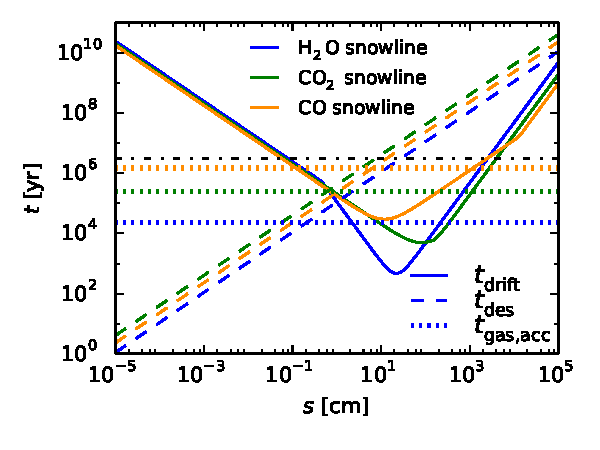
\includegraphics[width=0.7\textwidth]{figures/drift_timescales_betaS1_gas_acc_new2.pdf}
%\vspace{-0.5in}
\caption{Relevant timescales for dynamical effects in the desorption process: $t_{\rm drift}$ (solid lines), $t_{\rm des}$ (dashed lines) and $t_{\rm gas, acc}$ (dotted lines). The timescales are calculated at three representative locations, i.e. the H$_2$O, CO$_2$ and CO snowlines in the static disk. For our choice of parameters, the snowlines are located at $\sim$0.7 AU (blue lines), $\sim$8.6 AU (green lines) and $\sim$59 AU (red lines), respectively. The horizontal dot-dashed line represents a typical disk lifetime of 3 Myr. The particle size ordering at the minimum $t_{\rm drift}$ is not monotonic in snowline distance due to different drag regimes for those particle sizes at the snowline locations (Epstein drag at the H$_2$O and CO$_2$ snowlines, and Stokes drag at the CO snowline). Similarly, the ordering of $t_{\rm des}$ is not monotonic in snowline distance due to the non-monotony in mean molecular weight between H$_2$O, CO$_2$ and CO (18 $m_{\rm p}$, 44 $m_{\rm p}$ and 28 $m_{\rm p}$, respectively). Radial drift and gas accretion affect desorption in the regions where their respective timescales, i.e. $t_{\rm drift}$ and $t_{\rm gas, acc}$, are comparable to the desorption timescale $t_{\rm des}$.} 
\label{fig:timescales}
\end{figure}

For simplicity, we calculate the radial drift timescale, $t_{\rm drift}$, for an irradiated disk in this section, but most of our conclusions hold true for an evolving disk as well. Figure \ref{fig:timescales} shows $t_{\rm des}$, $t_{\rm drift}$ and $t_{\rm gas, acc}$ as a function of particle size at three different locations in the disk, corresponding to the H$_2$O, CO$_2$ and CO snowlines in the static disk. As expected, micron-sized particles desorb on very short timescales of $\sim 1-1000$ years in the close vicinity of their respective snowlines, since the desorption rate depends exponentially on temperature and hence on disk location (see Equation \ref{eq:Rdes}).  On the other hand, their radial drift timescale exceeds the typical disk lifetime of a few Myr by several orders of magnitude due to their strong coupling with the gas. Thus for small particles in an irradiated disk, the snowline locations and the C/O ratio are the same as for a static disk (see Figure 1 from \citealt{oberg11}). This is not true for an evolving disk, however, where gas accretion causes even micron-sized particles to drift significantly before desorbing, as we show in section \ref{sec:snowlines}. At the other extreme, kilometer-sized particles are unaffected by gas drag and have long desorption timescales ($\gg$1 Myr ), and the snowline locations and C/O ratio remain unchanged in this case as well. This is true for both irradiated and evolving disks, since large planetesimals are decoupled from the gas and hence unaffected by gas accretion onto the host star. 

In the particle size regime for which (1) $t_{\rm drift} \lesssim t_{\rm des} \lesssim t_{\rm d}$ ($t_{\rm d}=3$ Myr is the disk lifetime), i.e. for $\sim$$0.5$ cm $\lesssim s \lesssim$ $1000$ cm, or (2) $t_{\rm gas, acc} \lesssim t_{\rm des} \lesssim t_{\rm d}$, i.e. for $\sim$$0.1$ cm $\lesssim s \lesssim$ $10$ cm, radial drift or gas accretion (or both) are faster than thermal desorption, which is of particular interest for our purposes. We note that $t_{\rm gas, acc}<t_{\rm d}$ always holds true. Particles of sizes that satisfy the requirements above will drift significantly due to radial drift or gas accretion before desorbing, thus moving the H$_2$O, CO$_2$ and CO snowlines closer towards the central star and changing the C/O ratio throughout the disk. We quantify these effects in sections \ref{sec:snowlines} and \ref{sec:COratio}.



%\emgr{Calculate timescale for radial drift following Chiang \& Youdin (2010). Calculate desorption timescale following Hollenbach et al. (2009). Estimate gas accretion timescale for a given $\alpha$. Important: mention that, for simplicity and illustrative purposes, these calculations are performed for a passive disk. Show plot with the timescales as a function of particle size at different snowlines to show the regime in which drift matters}.



\section{Snowline Locations}
\label{sec:snowlines}





In this section we use the model described in section \ref{sec:model} to quantify the effects of radial drift (irradiated disk) or radial drift and gas accretion (evolving disk) on the snowline location, for dust particles of different sizes composed of either H$_2$O, CO$_2$ or CO. Specifically, we determine a particle's final location (i.e., where the particle either fully desorbs or remains at its initial size due to having a desorption timescale longer than the time at which we stop the simulation) as a function of its initial position in the disk, after the gas disk has dissipated. The disk lifetime, $t_{\rm d}$, is particularly relevant since the timescale for giant planet formation must be less than or equal to $t_{\rm d}$. The snowline locations at $t=t_{\rm d}$ throughout the protoplanetary disk determine the disk C/O ratio in gas at this time, and thus the C/O ratio in giant planet atmospheres that have formed \textit{in situ}, before planetesimal accretion or core dredging.   



For each species $x$, we determine the final location in the disk of a particle of initial size $s_0$ by solving the following system of coupled differential equations:

\begin{subeqnarray}
\label{eq:ddt}
\frac{ds}{dt} &= & - \frac{3 \mu_x m_{\rm p}}{\rho_{\rm s}} N_x R_{\rm des, x}  \slabel{eq:dsdt} \\
\frac{dr}{dt} &=& \dot{r} \slabel{eq:drdt},
\end{subeqnarray}
where the desorption rate $R_{\rm des, x}$ for each particle type (i.e., composed of H$_2$O, CO$_2$ or CO) is evaluated at $T=T(r)$, and the radial drift velocity $\dot{r}$ is given by Equation (\ref{eq:rdotpas}) for an irradiated disk and Equation (\ref{eq:rdotact}) for an evolving disk. Equations (\ref{eq:dsdt}) and (\ref{eq:drdt}) describe the coupled desorption and radial drift, and can be derived straightforwardly from Equation (\ref{eq:tdes}). Our initial conditions are $s(t_0)=s_0$ and $r(t_0)=r_0$, where $t_0$ is the initial time at which we start the integration and $r_0$ is the initial location of the particle.  We choose $t_0=1$ year, but our result is independent on the initial integration time as long as $t_0 \ll t_{\rm d}$. The desorption timescale $t_{\rm des}$ will then satisfy $s(t_{\rm des})=0$, from which we can determine the desorption distance $r_{\rm des}=r(t_{\rm des})$.

%As we show in Section \ref{sec:COratio}, a drifting particle that desorbs will do so almost instantaneously and will lose most of its mass very close to the distance at which it fully evaporates. 

%Thus a particle's final location will depend on whether a grain initially at a certain distance is completely desorbed or not within the disk lifetime of 3 Myr. For example, larger grains take longer to desorb and hence are more likely to not evaporate fully in a given timeframe. 



We define the final position of a grain as the disk location it has reached after $t_{\rm d}=3$ Myr, or the radius at which it completely desorbs if that happens after a time shorter than 3 Myr.  Figure \ref{fig:snowlines} shows our results for H$_2$O, CO$_2$ and CO particles, for both an irradiated and an evolving disk. We do not show the results for the viscous disk as they would complicate the plot without adding any qualitative insight ---  the results for the viscous disk are quantitatively similar with those of the evolving disk for the CO$_2$ and CO particles, but they are different for the H$_2$O grains, since accretion heating will push the H$_2$O snowline outwards (see Section \ref{sec:COratio}). We also show the static snowlines for comparison, which are calculated by balancing adsorption and desorption \citep{hollenbach09}. %We do not show the equivalent result for the steady-state active disk since The trends are qualitatively the same as for the active disk with the temperature profile given by Equation (\ref{eq:diskT}), but we discuss the C/O ratio steady-state active disk results in Section \ref{sec:COratio}. 
Kilometer-sized bodies do not drift or desorb during the disk lifetime neither for an irradiated nor for an evolving disk. Similarly, micron- to mm-sized particles in the irradiated disk do not drift and only %or 
desorb if %unless 
they are located inside the static snowlines. %This is not in contradiction with the desorption timescales for small particles from Figure \ref{fig:timescales}, since small grains only desorb fast at or nearby their respective snowlines, as mentioned in Section \ref{sec:timescales}.  [don't think this is needed, but Til or Ruth might think otherwise]
In an evolving disk, however, micron-to mm-sized grains do drift significantly since they move at the same velocity as the accreting gas. For $0.5$ cm $\lesssim s_0 \lesssim$ 700 cm in an irradiated disk and $0.001$ cm $\lesssim s_0 \lesssim$ 700 cm in an evolving disk, we notice that particles of initial size $s_0$ desorb at a %fixed distance 
particle size dependent radius $r_{\rm des}$ regardless of their original location in the disk. In fact, the only grains that will both drift and evaporate are those that reach their fixed final location (represented by the horizontal curves in Figure \ref{fig:snowlines}) within the disk lifetime. We show in section \ref{sec:COratio} that this result is essential in determining the C/O ratio throughout the disk for different particle sizes. 

Another interesting feature of Figure \ref{fig:snowlines} is that particles above a certain size ($\sim$7 m for our choice of parameters) all desorb at the same distance. This is due to the fact that once the large bodies pass the static snowline, they first lose mass, thus eventually following the same evolutionary track as the meter-sized bodies and evaporating at the same location.




Intuitively, this fixed $r_{\rm des}$ should be the location in the disk for which $t_{\rm drift} \sim t_{\rm des}$, given an initial particle size. We can calculate this location analytically by equating Equations (\ref{eq:tdes}) and (\ref{eq:tdrift}) and solving for $r=r_{\rm des}(s)$ for a given particle size $s$. Figure \ref{fig:an_vs_actual} shows $r_{\rm des}$ calculated analytically using the prescription above as a function of the actual desorption distance calculated numerically. We display this result for the range of particle sizes that desorb at a fixed distance in an irradiated and an evolving disk (see Figure \ref{fig:snowlines}). We notice that the analytic approximation accurately reproduces the numerical result for most cases of interest, but it deviates for particles larger than $s \gtrsim10$ cm. For small particles with $\tau_{\rm s} \ll 1$, $t_{\rm drift}$ is a power-law in $r$ (for our parameters, $t_{\rm drift} \propto r^{-1/14}$ for the irradiated disk in the Epstein drag regime), and the Equation set (\ref{eq:ddt}) has an explicit analytic solution (see \App{app:tdriftan}). Once particles are large enough so that $\tau_{\rm s} \sim 1$, $t_{\rm drift}$ has a more complicated dependence on $r$ (see Equation \ref{eq:ts}), and the coupled drift-desorption differential equations have to be integrated numerically to obtain an accurate result. 

\begin{figure}[H]
\centering
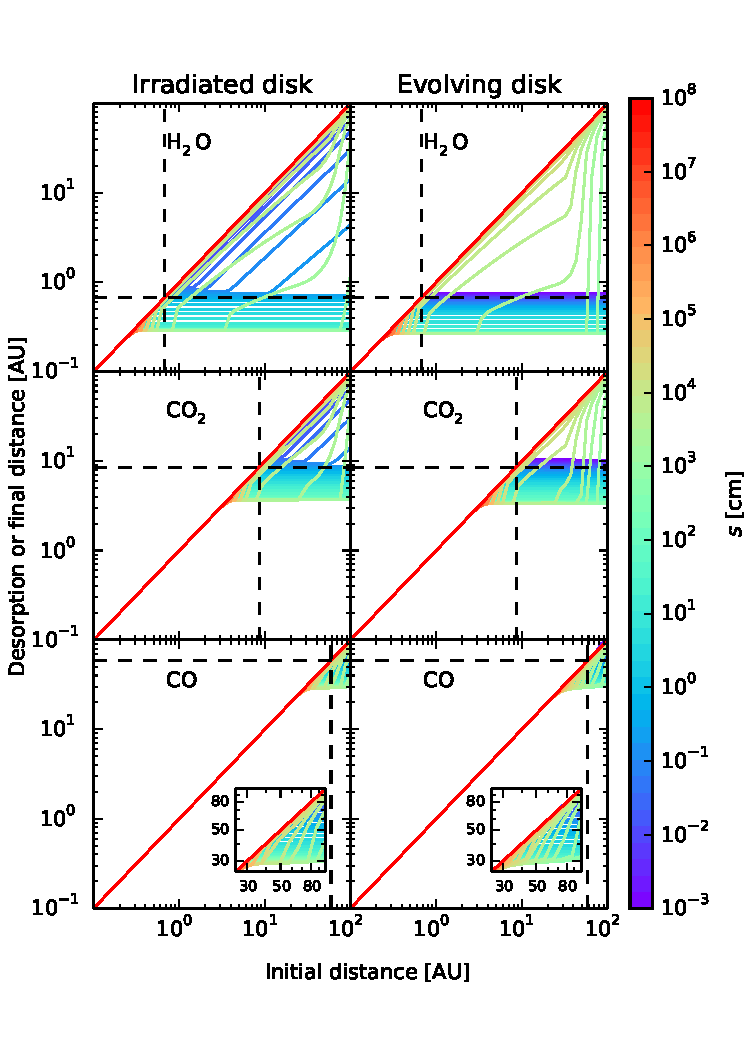
\includegraphics[width=0.8\textwidth]{figures/desorption_distance_passive_active_colorbar_test2.pdf}
%\vspace{-0.5in}
\caption{Desorption distance (if a grain fully desorbs; horizontal lines) or final distance (if a grain does not fully desorb; diagonal lines for particles that do not drift and non-horizontal, non-diagonal lines for particles that drift), as a function of a particle's initial location in the disk, for a range of particle sizes, and for both an irradiated disk (left panels) and an evolving disk (right panels). The desorption distance is calculated for particles composed of H$_2$O (top panels), CO$_2$ (middle panels) and CO (bottom panels). The desorption distance for a static disk is shown for comparison (dashed vertical and horizontal lines). The particle size increases from $10^{-3}$ cm to $10^8$ cm as indicated by the color bar. For a particle of a given initial size that entirely desorbs during $t_{\rm d}=3$ Myr, the desorption distance is the same regardless of the particle's initial location.} 
\label{fig:snowlines}
\end{figure}

\begin{figure}[H]
\centering
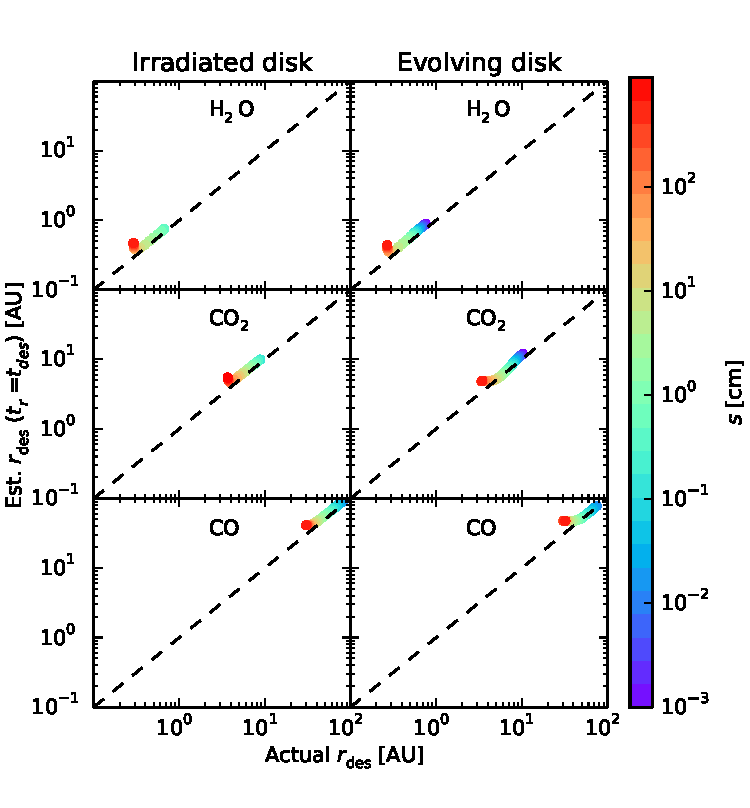
\includegraphics[width=\textwidth]{figures/desorption_distance_actual_vs_estimated_passive_active_new.pdf}
%\vspace{-0.5in}
\caption{Desorption distance estimated from analytic calculations (see text) as a function of the desorption distance calculated numerically, for the range of particle sizes that desorb at a fixed distance regardless of their initial location (see Figure \ref{fig:snowlines} and text). The estimate is performed for an irradiated disk (left panels) and an evolving disk (right panels).  The particles are composed of H$_2$O (top panels), CO$_2$ (middle panels) and CO (bottom panels). The analytic approximation is in good agreement with the numerical result for most cases, with the exception of larger particles, $s \gtrsim 10$ cm (see text).}
\label{fig:an_vs_actual}
\end{figure}


%This is due to the fact that large bodies lose their mass as they desorb until they reach the same size as the smaller, meter-sized particles, thus eventually following the same evolutionary track as the meter-sized bodies and evaporating at the same location. 

\begin{figure}[H]
\centering
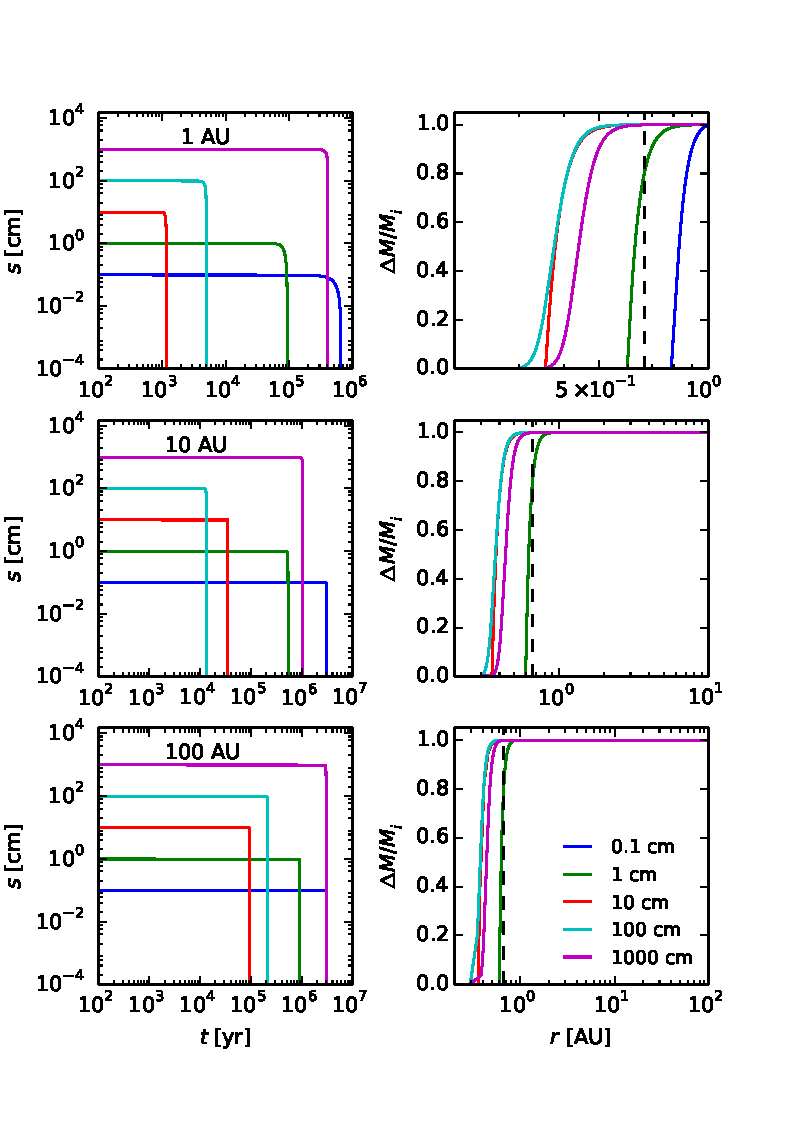
\includegraphics[width=0.8\textwidth]{figures/s_t_a.pdf}
%\vspace{-0.5in}
\caption{Left panels: size of desorbing H$_2$O particles as a function of time, for different initial particle sizes and for three initial locations in an irradiated disk: 1 AU (top left), 10 AU (middle left) and 100 AU (bottom left). Particles desorb almost instantaneously. Right panel: fractional mass of the desorbing particles as a function of the particle's location as it drifts, for different initial particle sizes, and at the same initial locations presented in the left panel. Particles lose most of their mass very close to the distance at which they fully desorb. The static H$_2$O snowline is shown for reference (dashed vertical lines).}
\label{fig:s_t_a}
\end{figure}

Given $r_{\rm des}$, we need to only calculate the distance over which particles desorb to determine the location of a snowline. Figure \ref{fig:s_t_a}, left panels, shows the size evolution with time for H$_2$O particles of various initial sizes, starting at three different initial locations in an irradiated disk. Once solid H$_2$O particles begin to evaporate, they do so almost instantly for all explored particle sizes and initial locations.



The right panels of Figure \ref{fig:s_t_a} show that the drifting grains lose most of their mass in a very narrow distance range; moreover, this distance is the same for a given initial particle size, no matter where the particle started drifting at the time $t_0$ when the simulation is started. Figure \ref{fig:s_t_a} thus demonstrates that solid particles that drift and fully desorb during the lifetime of the protoplanetary disk do so (1) instantaneously, and (2) at a fixed stellocentric distance, regardless of their initial location in the disk. 
It follows that the H$_2$O, CO$_2$ and CO snowlines are fixed for a given initial particle size and disk model. Both of these conclusions remain valid for an evolving and a viscous disk, as well as for particles composed of CO$_2$ or CO, but the snowline locations will vary between the three disks for a given initial particle size (see Section \ref{sec:COratio}). If we do not take into account the time dependence of the mass accretion rate and stellar luminosity (see Section \ref{sec:disk}), the C/O ratio will then only depend on disk properties, grain size, and the abundance of H$_2$O, CO$_2$ and CO relative to the H$_2$ abundance in the disk midplane, and {\it not} directly on the disk age when only considering drift, accretion and desorption.  %\emgr{I've yet to figure out why there is a discrepancy for the small grains. I'll keep thinking about it, but for now I'll leave it as it is since I don't want to give a false explanation just to have one.} 



%\emgr{I didn't write the text for Figure 4 since we haven't yet decided if in the end we will include it in some form. We can }

%\begin{figure}[h!]
%\centering
%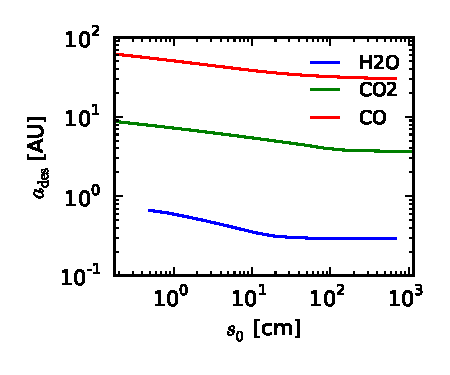
\includegraphics[width=0.5\textwidth]{../../figs/desorption_distance_vs_s.pdf}
%%\vspace{-0.5in}
%\caption{Desorption distance as a function of initial particle size, for the range of particles that desorb at a fixed distance regardless of initial location (see Figure \ref{fig:snowlines}). \textbf{Figure belongs to section 3.} \emgr{This is a figure that I'm not sure we should include, since it doesn't really provide that much useful inside. If we did include it though, there would be two panels both for the passive and the active disk. The caption is not complete since the active disk panel is not yet there.}}  %  (See text for a description of evolution to yet higher masses.) 
%\label{fig:r_vs_s}
%\end{figure}

%\emgr{Present the equation set that you are solving, $dr/dt=\dot{r}$, $ds/dt=...$. I don't think it is necessary to describe in detail the numerical method of solving the equations since it's pretty straightforward. Present the pretty rainbow plots side by side for passive and active disks, and highlight the differences. Insert the plots that shows that for the intermediate size particles, the desorption distance can be estimated analytically with good accuracy. Maybe also include the plot showing the desorption distance as a function of particle size, both for passive and active disk. Split into subsections?}


\section{C/O Ratio Estimates}
\label{sec:COratio}



Given our results in Section \ref{sec:snowlines}, a disk's C/O ratio in mainly affected by the snowline location for the particle size housing the most mass in ice.
%We now use our model and the results of Section \ref{sec:snowlines} to determine the H$_2$O, CO$_2$ and CO snowline locations in disks with static chemistry that experience radial drift of solids and gas accretion onto the central star. Using this and assuming a fixed abundance relative to hydrogen for each of these volatiles, we can then estimate the C/O ratio throughout the disk as a function of the particle size. 
Realistic grain size distributions in disks are dominated by large grains (e.g., \citealt{dalessio01}, \citealt{birnstiel12}). In Figure \ref{1fig:CO_ratio}, we display the H$_2$O, CO$_2$, and CO snowline locations as a function of particle size for disks with static chemistry that experience radial drift of solids and gas accretion onto the central star.  The minimum snowline distance for a disk is given by the curve corresponding to the maximum particle size it hosts.  For grains that have grown to radii larger than $\sim$7 m and are able to drift and desorb, the $\sim$7 m snowline applies (see Section 3).  %Thus for a given grain size distribution with a maximum particle size, we can pick out the appropriate minimum snowline locations from Figures \ref{fig:snowlines} and \ref{fig:CO_ratio}, as we show later in this section. 

\begin{figure}[H]
\centering
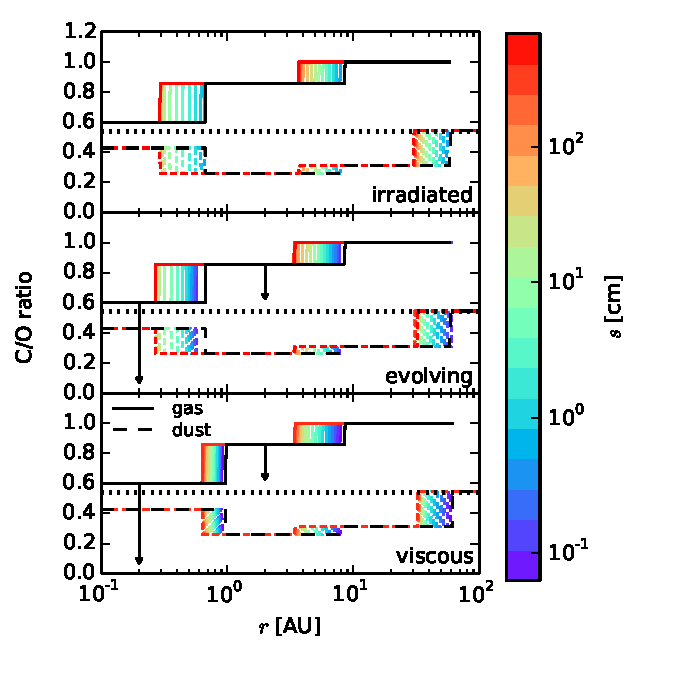
\includegraphics[width=0.7\textwidth]{figures/C_O_ratio_passive_active_disk_many_colorbar_complete_new2.pdf}
%\vspace{-0.5in}
\caption{Estimated C/O ratio in gas (solid lines) and in dust (dashed lines) for an irradiated disk (top panel), an evolving disk (middle panel) and a viscous disk (bottom panel).
%, for the range of particle sizes that desorb at a fixed distance regardless of their initial location in the disk. 
The particle size increases from $\sim$0.05 cm to $\sim$700 cm as indicated by the color bar. The horizontal dotted line represents the stellar value of 0.54. The black lines represent the C/O ratio in gas (solid black line) and dust (dashed black line) for a static disk, with the temperature profile given by Equation (\ref{eq:diskT}) for the top two panels and by Equation (\ref{eq:activeT}) for the bottom panel. 
%The snowline location moves inward as the particle size increases. 
%The curves exterior to the static snowline represent desorption distances in the absence of readsorption.  %Taking  readsorption into account, the snowlines for these particle sizes are in fact coincident with the static snowline. 
For both the evolving and the viscous disk, the movement of desorbed CO$_2$ gas inside the CO$_2$ snowline, and of desorbed CO$_2$ and H$_2$O gas inside the H$_2$O snowline due to gas accretion will increase the amount of oxygen gas inside the respective snowlines and thus reduce the gas C/O ratio, as shown by the arrows.}
%, with the decrease more significant interior to the H$_2$O snowline.}
\label{1fig:CO_ratio}
\end{figure}

%[I think a sentence is missing here outlining what you need to establish to calculate the C/O ratio, i.e. the connection between the preceding and the next sentence is not obvious.] 

%Figure \ref{fig:s_t_a}, left panels, shows the size evolution with time for H$_2$O particles of various initial sizes, starting at three different initial locations in a passive disk. Once solid H$_2$O particles begin to evaporate, they do so almost instantly for all explored particle sizes and initial locations. %, although the time $t_{\rm des}$ at which a particle of a given initial size desorbs depends on its initial distance. 
%A particle located at the initial time $t_0$ at a distance such that $t_{\rm des}>t_{\rm d}$ will therefore not desorb during the disk lifetime, but our model assumes that particles drift continuously at any location in the disk. [not sure you need to explain this]
%The right panels of Figure \ref{fig:s_t_a} show that the drifting grains lose most of their mass in a very narrow distance range; moreover, this distance is the same for a given initial particle size, no matter where the particle started drifting at the time $t_0$ when the simulation is started. Figure \ref{fig:s_t_a} thus demonstrates that solid particles that drift and fully desorb during the lifetime of the protoplanetary disk do so (1) instantaneously, and (2) at a fixed stellocentric distance, regardless of their initial location in the disk. 
%It follows that the H$_2$O, CO$_2$ and CO snowlines are fixed for a given initial particle size and disk model (passive or active)\footnote{Both of these conclusions remain valid for an active disk and for particles composed of CO$_2$ or CO.}. The C/O ratio will then only depend on disk properties, grain size, and the abundance of H$_2$O, CO$_2$ and CO relative to the H$_2$ abundance in the disk midplane, and {\it not} directly on the disk age when only considering drift, accretion and desorption. 


%In Section \ref{sec:snowlines}, we showed that solid particles that drift and fully desorb during the lifetime of the protoplanetary disk do so (1) instantaneously, and (2) at a fixed stellocentric distance, regardless of their initial location in the disk. Figure \ref{fig:s_t_a} confirms both of these effects. The left panels show the size evolution with time for H$_2$O particles of various initial sizes, starting at three different initial locations in a passive disk \footnote{Our conclusions remain valid for an active disk and for particles composed of CO$_2$ or CO.}.  Indeed, the solid H$_2$O particles evaporate almost instantly, although the time $t_{\rm des}$ at which a particle of a given initial size desorbs depends on its initial distance. A particle located at the initial time $t_0$ at a distance such that $t_{\rm des}>t_{\rm d}$ will therefore not desorb during the disk lifetime. However, our model assumes that particles drift continuously at any location in the disk. Therefore, a particle that can fully desorb during the disk lifetime for at least one initial location will always desorb, at a fixed distance as discussed in Section \ref{sec:snowlines} and displayed in Figure \ref{fig:snowlines}. The right panels of Figure \ref{fig:s_t_a} show that the drifting grains lose most of their mass in a very narrow distance range; moreover, this distance is the same for a given initial particle size, no matter where the particle started drifting at the time $t_0$ when the simulation is started. Figure \ref{fig:s_t_a} thus proves claims (1) and (2) above. 


Drift and gas accretion affect the C/O ratio in a disk both because they move the snowline locations of the main C and O carriers  and because they cause solids and gas---which contain different proportions of C and O---to move inward at different rates.  As shown in Section 3, the snowline locations depend on disk age only indirectly, through changes in disk properties and grain size.  The C/O ratio is a function of the locations of the snowlines and the abundances of H$_2$O, CO$_2$, and CO relative to the H$_2$ abundance in the disk midplane.   These abundances evolve over time as solids and gas move inward at different rates.

Figure \ref{1fig:CO_ratio} shows the estimated C/O ratio in gas and dust as a function of semimajor axis for an irradiated disk, an evolving disk, and a viscous disk, under the simplifying assumption that the abundance relative to hydrogen for each volatile is fixed, so that drift and accretion affect only the locations of the snowlines. We use the relative number densities of C and O in their different molecular forms (H$_2$O, CO$_2$ and CO) from Table 1 of \citet{oberg11}.  Snowline locations correspond to $r_{\rm des}$ in Figure \ref{fig:snowlines}, representing the location at which particles desorb in the absence of readsorption.  The C/O ratio for a static disk, where desorption and readsorption balance \citep{hollenbach09}, is shown as a guideline. We note that the true snowline for particles with $r_{\rm des}$ outside the static snowline is the static snowline itself---thus only particles with initial sizes larger than $\sim$0.05 cm are plotted in the three panels, as particles that form snowlines at larger distances (cf. Figure \ref{fig:snowlines}) are not true snowlines.


Before discussing the quantitative aspects of this plot, it is essential to acknowledge that our estimates for the C/O ratios in the evolving and viscous disks ignore the movement of the desorbed ices with the accreting gas---the relative fluxes of the volatiles in gaseous and solid form will affect the relative abundance of C and O in gas and dust throughout the disk. As demonstrated in Figure \ref{fig:s_t_a}, this will not affect the snowline locations for particles of a given size, but will change the shape of the C/O curves in between the various snowlines. For example, for the disk parameters and particle sizes displayed in Figure \ref{1fig:CO_ratio}, water molecules in solid particles drift up to $\sim$1000 times faster across the H$_2$O snowline than do molecules of CO and CO$_2$ vapor that are entrained in the accreting gas.  This differential inward motion will result in an increased oxygen gas abundance inside the H$_2$O snowline, and thus a (in some cases much) lower gaseous C/O ratio in this region. Conversely, oxygen gas inside the water snowline will be depleted compared to the static disk if H$_2$O particles grow to planetesimal size and stall their migration between the H$_2$O and CO$_2$ snowlines, leaving only gaseous CO and CO$_2$ to accrete inward.  Growth of large planetesimals can therefore increase the C/O ratio in the inner disk. 

%\textbf{Our premise that each volatile has a fixed abundance at every location in the disk yields good approximations for the C/O ratio in an irradiated disk --- our model assumes a constant influx of particles at any given radius, implying that the solid surface density of a given volatile, and therefore the amount of desorbed vapor, remain constant with semimajor axis. For the evolving and viscous disks, the C/O ratio in gas may decrease due to the decline in the surface density of solids with time. Thus both the relative fluxes of the volatiles and the decrease in solid ice abundances will lower the C/O ratio in evolving and viscous disks, as indicated by the arrows in Figure \ref{fig:CO_ratio}. However, a high gas-phase C/O ratio is maintained further in for all disks compared to a static disk, since drift and gas accretion cause the ices to desorb closer to the host star.}



%\textbf{Desorption is taken into account in the figure, and fundamentally the elevated C/O ratio interior to the static CO2 and H2O snowlines are simply due to the inward mobility of the snowlines (desorption fronts) due to drift and accretion flows. Qualitatively this scenario should be robust to changes in total abundances throughout the disk, i.e. at e.g. the �dynamic� CO2 snowlines, the rapid return of CO2 into the gas-phase (during CO2 desorption) will reduce the C/O ratio interior to the CO2 dynamic snowline, while no major change in gas-phase composition and therefore C/O ratio is expected between the static and dynamic snowlines.

%As the referee notes, we do operate under the simplifying assumption that the total (ice+gas) abundances are the same at each radius after ices have migrated. This is a good
%approximation for the irradiated disk, given that this model by definition presents a constant influx of particles at any given radius while the gas is static, and thus the ice+gas surface density should remain constant. For the evolving disk, we agree with the referee that this is not a good approximation. In evolving disks, the gas-phase C/O ratio may decrease everywhere interior to the CO2 and H2O desorption fronts due to the decrease in the surface density of solids with time at any given radius. In the steady-state viscous disk, the solid abundances at a fixed radius are constant, given that this model is
%not time-dependent, but the solid/gas ratio is not constant, which can result in a substantially lower C/O ratio interior to the H2O and CO2 snowlines compared to the static case (as indicated by the arrows in the figure).

%These caveats are important and we have explained and clarified them further in the next. We have also clarified that the main purpose of this figure is to show the different snowline locations in static and dynamic disks, and thus where in the disk C/O is reduced or increased rather than providing a quantitative estimate of how big or small that increase/decrease is.}


Figure \ref{1fig:CO_ratio} plots snowline curves for particle sizes $\sim0.5$ cm $\lesssim $s$ \lesssim$ 7m.  In the outermost disk, H$_2$O, CO$_2$, and CO all solidify.  Hence, relative drift across the CO snowline can alter only the abundances of volatiles between the CO$_2$ and CO snowlines, but not the C/O ratio in this region.  Interior to the CO$_2$ snowline, however, relative drift is important. 
We have found that the largest drifting particles in our model ($\sim$7 m) drift faster than the gas at both the H$_2$O and CO$_2$ snowlines. We thus conclude that the C/O ratio interior to the H$_2$O and CO$_2$ snowlines in our evolving and viscous disks will be lower than in the static disk, due to the additional oxygen added to the gas by desorbing H$_2$O and CO$_2$.  For these particle sizes, our calculated C/O ratio is an upper limit,  as indicated by the arrows in Figure \ref{1fig:CO_ratio}.

Fundamentally, the elevated C/O ratios interior to the static H$_2$O and CO$_2$ snowlines are simply caused by the inward movement of the snowlines due to radial drift and gas accretion. Qualitatively, this scenario should be robust to changes in total abundances throughout the disk --- for example, at the dynamic (non-static) CO$_2$ snowlines, the rapid return of CO$_2$ into gas-phase during CO$_2$ desorption will reduce the C/O ratio interior to the CO$_2$ dynamic snowline, while no major change in gas-phase composition, and therefore C/O ratio, is expected between the static and dynamic snowlines.

As noted earlier, we assume that the total (ice and gas) abundance of each volatile is the same at every radius after ices have migrated. This is a good approximation for the irradiated disk, given that this model, by definition, presents a constant influx of particles at any given radius while the gas is static, and thus the ice and gas surface density remain constant. For the evolving disk, the gas-phase C/O ratio may decrease everywhere interior to the H$_2$O and CO$_2$ snowlines due to the decline in the surface density of solids with time at any given radius. For the viscous disk, the solid abundances at a fixed radius are constant, given that this model is not time-dependent, but the gas-to-solid ratio is not constant, which can result in a substantially lower C/O ratio interior to the H$_2$O and CO$_2$ snowlines compared to the static case (as indicated by the arrows in Figure \ref{1fig:CO_ratio}). The main goal of Figure \ref{1fig:CO_ratio}, however, is to show the different snowline radii in static and non-static disks, and therefore the locations in the disk where the gas-phase C/O ratio is reduced or increased, rather than provide a quantitative estimate of the magnitude of the C/O increase or decrease.


%We use the relative number densities of C and O in their different molecular forms (H$_2$O, CO$_2$ and CO) from Table 1 of \citet{oberg11}. Figure \ref{fig:CO_ratio} shows the estimated C/O ratio in gas and dust as a function of semimajor axis for a passive disk, an active disk, and an active disk accretionally heated. The C/O ratio for a static disk is shown as a guideline. We note that particles desorbing outside the static snowline will not form snowlines, since our calculation of the desorption distance does not account for readsorption  \citep{hollenbach09}. 

%Before discussing the quantitative aspects of this plot, it is essential to acknowledge that our estimates for the C/O ratios in the active disks ignore the movement of the desorbed ices with the accreting gas --- the relative fluxes of the volatiles in gaseous and solid form will affect the relative abundance of C and O in gas and dust throughout the disk. As demonstrated in Figure \ref{fig:s_t_a}, this will not affect the snowline locations for particles of a given size, but will change the shape of the C/O curves in between the various snowlines. Specifically, the gas C/O ratios may be significantly lower inside the H$_2$O and CO$_2$ snowlines for the active disks, depending on the gas accretion rate, due to the additional oxygen contained by H$_2$O and CO$_2$ vapor that moves together with the accreting gas and crosses their respective snowlines.

%e thus present this result for the C/O ratio primarily as a visual comparison with previous work \citep{oberg11} and note that our estimates for the C/O ratio in the active disks are not quantitatively accurate at all disk locations. Future work will address this issue.   

 %The plot is consistent with Figure \ref{fig:snowlines}. 
The snowline locations in these disks exhibit several interesting features. For the irradiated disk, only grains larger than $\sim$0.5 cm drift, desorb and thus move the snowline compared to the static disk. In contrast, even $\sim$micron-sized grains drift and desorb for the evolving disk, since they flow towards the host star together with the accreting gas. For the same particle size, the snowline locations are slightly closer to the central star in the evolving disk, due to the fact that the accreting gas adds an additional component to the drift velocity of the solids (cf. Equation \ref{eq:rdotact}). The addition of accretional heating in the viscous disk moves the H$_2$O snowline outwards. This is due to the fact that accretional heating dominates in the inner disk, where high temperatures cause the grains to evaporate further away from the star. Once $r\gtrsim1-2$  AU, stellar irradiation dominates the thermal evolution of the disk, and therefore the CO$_2$ and CO snowlines locations are the same as in the evolving and viscous disks. 

Perhaps the most interesting feature is the fact that the snowlines are pushed inwards as the grain size increases. While the plot only shows the snowlines and C/O ratio for particle sizes up to $\sim$7 m, we have found that %almost kilometer-sized boulders are able to drift and desorb for both the passive and the active disk. B
bodies larger than $\sim$7 m evaporate at the same location as the meter-sized planetesimals (see Section \ref{sec:snowlines}). However, the contribution of kilometer-sized bodies to the snowline location is modest, since they only drift if they are located very close to the snowline.
%[new sentence explaining that their contribution may not be very big due to their modest drift.] though 
%only the kilometer-sized boulders that are very close to the snownlines will contribute to determining the snowline location. 
Thus the innermost snowlines (depicted in red in Figure \ref{1fig:CO_ratio}) set the limit on how close in the H$_2$O, CO$_2$ and CO snowlines can be pushed due to radial drift and gas accretion on to the host star. For a grain size distribution with a maximum particle size different than our model, one can pick out the appropriate minimum snowline locations from this plot.%Realistic grain size distributions in disks are dominated by large grains (e.g., \citealt{dalessio01}, \citealt{birnstiel12}).  Thus for a given grain size distribution with a maximum particle size, we can pick out the appropriate minimum snowline locations from this plot. %Our model thus sets an inner limit to the snowline locations. %Therefore, the snowlines produced by the largest drifting solids in our model set the inner limit on the snowline locations and are insensitive to a particular grain size distribution --- for a given grain size .

% [the last sentence needs to be made more explicit, i.e. for a given grain size distribution with a maximum grain size a reader can now pick out the appropriate minimum snowline location from this plot]

For our choice of parameters, the minimum snowline radii are: $r_{\rm{H_2O}} \approx 0.3$ AU for the irradiated disk, $r_{\rm{H_2O}} \approx 0.26$ AU for the evolving disk and $r_{\rm{H_2O}} \approx 0.63$ AU for the viscous disk; $r_{\rm{CO_2}} \approx 3.7$ AU for the irradiated disk, $r_{\rm{CO_2}} \approx 3.4$ AU for both the evolving and the viscous disks; $r_{\rm{CO}} \approx 30$ AU for the irradiated and both the evolving and the viscous disks. For comparison, $r_{\rm{H_2O}} \approx 0.67$ AU\footnote{For the viscous disk, we calculated the static snowline location using the same temperature profile as that of the viscous disk, for consistency purposes. Thus $r_{\rm{H_2O}} \approx 0.98$ AU for the static disk in this scenario.}, $r_{\rm{CO_2}} \approx 8.6$ AU and $r_{\rm{CO}} \approx 59$ AU for the static disk. For the viscous disk model, which is the most realistic, radial drift and gas accretion push the snowline locations inwards by up to $\sim$$40$ \% for H$_2$O, by up to  $\sim$$60$ \% for CO$_2$, and by up to $\sim$$50$ \% for CO.  We note that the H$_2$O snowline in all disks is significantly closer to the host star compared with Solar system models, which place the H$_2$O snowline between $\sim$$2.7$ to $\sim$$3.1$ AU (\citealt{hayashi81}, \citealt{podolak04}, \citealt{martin12}). This is partially because we choose a colder disk model, as well as the fact that gas accretion rates decrease over time, moving the snowline location inwards (see also \citealt{garaud07} and Section \ref{sec:neglected}). \citet{min11} find that the location of the H$_2$O snowline is highly sensitive to the gas mass accretion rate $\dot{M}$ (equal to $10^{-8} M_{\odot}$ yr$^{-1}$ in our model) and the dust opacity $\kappa$ (Equation \ref{eq:opacity}). Higher values of $\dot{M}$ and $\kappa$ would increase the accretional component of the disk temperature (cf. Equation \ref{eq:Tdact}), which would push the H$_2$O snowline in the viscous disk outwards to match the Solar system snowline. At the same time, the snowline location in Solar type stars may be as close as $\sim$1 AU \citep{mulders15}, further in than the H$_2$O snowline in our Solar system.

 Observations of the CO snowline in TW Hya \citep{qi13} have found its location at a disk midplane temperature of 17 K (at 30 AU for the TW Hya specific temperature profile). The inferred  desorption temperature corresponds to the CO desorption temperature in a static disk, or to desorption from very small grains in an evolving disk, i.e. from grains that are too small to drift substantially. This suggests that the outer TW Hya disk is dominated by small grains, since larger particles would push the snowline location inwards, and therefore to higher desorption temperatures. This may seem contradictory to observations of grain growth in disks in general and in TW Hya in particular \citep{wilner00}. However, recent observations have revealed that grain growth is concentrated to the inner disk \citep{perez12} and outer disk snowlines may therefore be close to the ones expected in a static disk.


%\emgr{There will be 1-2 additional sentences for the third panel, the steady-state disk, once that finishes running.}





%\begin{figure}[h!]
%\centering
%\includegraphics[width=0.5\textwidth]{lala}
%%\vspace{-0.5in}
%\caption{C/O ratios for different particle size distributions... \textbf{Figure belongs to section 4.} (\emgr{It will probably be a multi-panel plot, for different particle size distributions, for both passive and active disk, and perhaps at different times for the active disk. Not yet unsure how that figure will look like since I don't have the results yet, so I'll leave the figure caption open for now.})}
%\label{fig:...}
%\end{figure}

%\emgr{Motivate the fact that we can calculate a sharp, fixed snowline for each particle size by inserting the plot that shows that particles desorb almost instantaneously at a fixed distance.  Then present the plots analogous to Fig. 1 in \"Oberg et al. (2011) for different particle sizes, based on the snowline locations obtained in the previous section, both for passive and active disk. Perhaps show it at different times in the gas disk evolution (i.e., not just at 3 Myr) for the active disk. Then assume a particle size distribution and show the interpolated result for the C/O ratio. Generalize the result using a transition disk (this part might also fit in the discussion section).}

%emgr{Present the flux equations used to keep track of the amount of C and O in gas and dust throughout the disk. Motivate the simplification of using a fixed particle sized, fixed timescale, and fixed desorption distance in the calculations by referring to the rainbow plot in the previous section and by inserting the plot that shows that particle desorb almost instantly at a fixed distance. Based on these assumptions, finally show the equivalent of Fig. 1 in \"Oberg et al. (2011) for different particle sizes, and at different times in the gas disk evolution (i.e., not just at 3 Myr) --- a multi-panel plot could be a good idea. Discuss the result, trends, etc. Ideally, have a final plot showing the results for a particle size distribution rather than for individual particles.}

\section{Discussion}
\label{sec:discussion}








\subsection{Generality of Results: Dependence on Disk Parameters}
\label{sec:incond}

In this section we investigate how variations in our fiducial parameters, the total disk mass, disk age, and disk structure, %the time in the disk evolution at which we determine 
affect the calculated snowline locations and the C/O ratio. %, affect our results. 
All previous results assumed a disk lifetime $t_{\rm d}=3$ Myr%is the most representative for our calculations, as this is the timeframe in which giant planets accrete their gaseous atmospheres 
, the typical disk lifetime and the expected time scale for giant planets to accrete their gaseous atmopsheres (e.g., \citealt{pollack96}, \citealt{piso14}). Some gas accretion may occur at earlier times, however,%However, protoplanetary cores start acquiring their envelope at earlier times, 
before the core is fully formed (e.g., \citealt{rafikov06}). Recent models such as aerodynamic pebble accretion \citep{lambrechts12} suggest that rapid core growth on timescales of $10^5$ years is possible. % which implies that the time when cores accrete their massive envelope may be at least an order of magnitude shorter than the disk lifetime. 
The composition of giant planet atmospheres, and specifically their C/O ratio, can thus depend on the abundance of H$_2$O, CO$_2$ and CO in gas at earlier times than $t_{\rm d}$ in the disk evolution. 

Figure \ref{fig:timeplots} shows the particle desorption or final distance as a function of a particle's initial location in the disk, for ice particles %grains 
of initial sizes of 10 cm and 1 m, composed of either H$_2$O, CO$_2$ or CO. These sizes are important since radial drift timescales are shortest for particles within this size range (see Figure \ref{fig:timescales}) --- these are the particles whose drift and desorption evolution should be most strongly affected by variations in disk conditions. We choose the evolving disk as a disk model, and we stop the simulations after $10^4$ yr, $10^5$ yr, 1 Myr and $t_{\rm d}=3$ Myr, respectively. %, to see how the snowline locations evolve with time and affect the C/O ratio. 
The most important result of these plots is that particles of a given size always desorb at the same disk radii, the 3 Myr snowline, regardless of simulation stopping time.  Particles %of a given size 
that start at large stellocentric distances do not desorb within the shorter timeframes, e.g. $10^4$ or $10^5$ years, but they do evaporate at a fixed radius if their initial location is closer to the host star. While the amount of material that moves through the disk changes with time, the radius at which particles desorb and 
the snowline locations are thus independent of the time elapsed, and %. Therefore, 
our results for the snowline locations are %not only valid at $t_{\rm d}$, but also throughout the earlier 
valid throughout the time evolution of the protoplanetary disk. 

\begin{figure}[H]
\centering
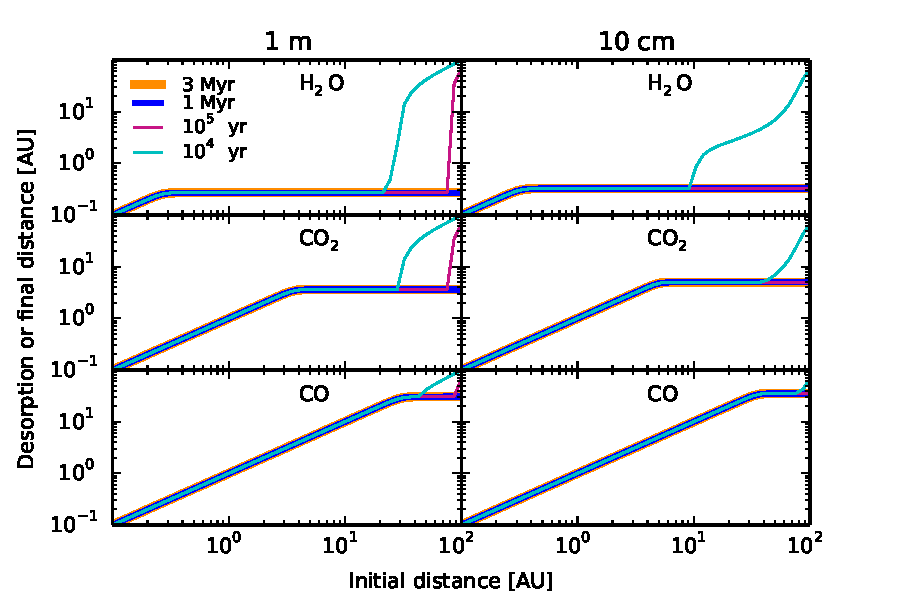
\includegraphics[width=\textwidth]{figures/time_plots.pdf}
%\vspace{-0.5in}
\caption{Desorption or final distance as a function of initial position in the disk for particles of initial size $s_0=1$ m (left panels) and $s_0=10$ cm (right panels), for grains composed of H$_2$O (top panels), CO$_2$ (middle panels) and CO (bottom panels). The evolution is shown at four representative timescales: $10^4$ yr (cyan curve), $10^5$ yr (purple curve), 1 Myr (blue curve), and 3 Myr, the disk lifetime (orange curve). For a given particle size, the desorption distance, and hence the H$_2$O, CO$_2$ and CO snowlines, have the same location regardless of the time at which the simulation is stopped.}
\label{fig:timeplots}
\end{figure}

We choose as a fiducial model a total disk mass $M=0.1 M_{\odot}$. Observationally, disk masses span at least an order of magnitude around Solar type stars %, but this number is not universally valid. From observations of the dust continuum, 
\citep{andrews13}. % find that a linear scaling $M \propto M_*$ is reasonable. Giant planets, however, have been detected around small stars (e.g., \citealt{montet14}), which can have masses as low as $M_* \sim 0.1 M_{\odot}$. 
We thus explore the effect of disk mass on the location of snowlines. Figure \ref{fig:varMd} shows the desorption or final distance as a function on the initial location of a H$_2$O particle with initial size of 1 m, for two total disk masses: $M=0.1 M_{\odot}$, our fiducial model, and $M=0.01 M_{\odot}$. Similarly to Figure \ref{fig:timeplots}, we perform our calculations for an evolving disk. The simulations are stopped after the same timeframes as those in Figure \ref{fig:timeplots}. The location of the H$_2$O snowline is the same for both disks (the same holds true for the CO$_2$ and CO snowlines). The C/O ratio is thus insensitive to the choice of $M$. We note that our conclusions regarding the disk age and total mass are only valid if the snowline itself does not move with time or disk mass (see also Sections \ref{sec:disk} and \ref{sec:neglected}).

\begin{figure}[H]
\centering
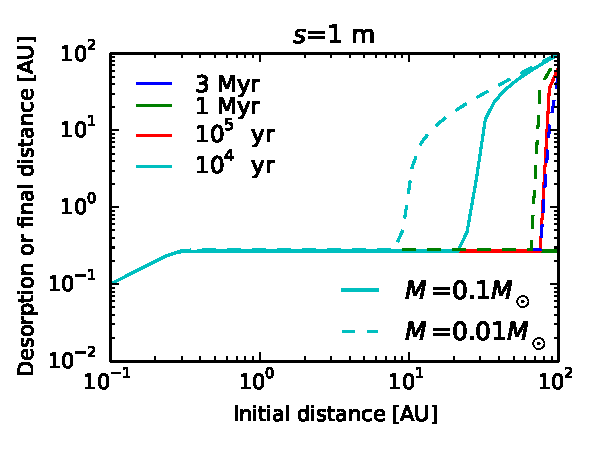
\includegraphics[width=0.7\textwidth]{figures/desorption_distance_varying_Md.pdf}
%\vspace{-0.5in}
\caption{Desorption or final distance as a function of initial position in the disk for H$_2$O particles of initial size of 1 m, for total disk masses $M=0.1 M_{\odot}$ (solid lines) and $M=0.01 M_{\odot}$ (dashed lines). The timescales at which we stop the simulations are $10^4$ yr (cyan curve), $10^5$ yr (red curve), 1 Myr (green curve) and 3 Myr (blue curve). A lower disk mass does not change the snowline location.}
\label{fig:varMd}
\end{figure}

%This result also has implications for transition disks, which have inner cavities significantly depleted of dust (e.g., \citealt{espaillat12}). Since the snowline locations are independent of disk mass, we expect transition disks to exhibit the same drift-desorption behavior as standard disks under the simplified assumptions of our model. 
%[Comment on differences, i.e. short time frames there is a difference because of smaller drift velocity in the lighter disk I presume.]

We also apply our evolving disk model to a transition disk, i.e. a protoplanetary disk with an inner cavity significantly depleted of gas. We choose a disk with an inner gap of radius $r_0=4$ AU, consistent with observations of TW Hya \citep{zhang13}, and with the gas surface density in the gap reduced by a factor of 1000. Figure \ref{fig:cavity} shows the desorption or final distance for a H$_2$O particle of initial size of 1 m, with the simulation stopped at the same timescales as in Figures \ref{fig:timeplots} and \ref{fig:varMd}. Particles that start at an initial distance interior to the gap drift towards the original snowline, while grains located exterior to the gap stop shortly after crossing the gap edge, due to the decrease in gas pressure inside the cavity, thus forming a snowline at $\sim$$3.8$ AU. This is qualitatively consistent with the observations of \citet{zhang13}, which show that the H$_2$O snowline is pushed outwards in a transition disk compared to a full disk. Our model framework is thus generally valid for more complicated disk structures as well.  

\begin{figure}[H]
\centering
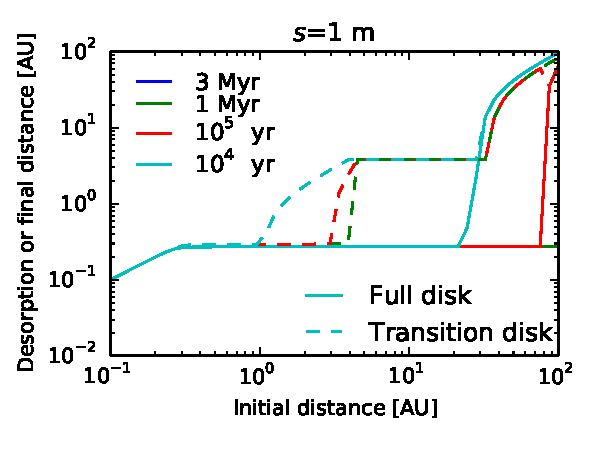
\includegraphics[width=0.7\textwidth]{figures/desorption_distance_transition_disk_1000.pdf}
%\vspace{-0.5in}
\caption{Desorption or final distance as a function of initial position in the disk for H$_2$O particles of initial size of 1 m, for our fiducial disk (solid lines) and for a transition disk with an inner cavity at $r_0=4$ AU (dashed lines). The timescales of the simulations and their color code are the same as in Figure \ref{fig:varMd}. Particles that start inside the cavity drift towards the original snowline, while particles that start outside the gap stop shortly after crossing the gap edge, due to being trapped in a pressure maximum.}
\label{fig:cavity}
\end{figure}

%[Need a sentence about how this makes the model framework also generally valid for more complicated disk structures.]



\subsection{Model Extensions}
\label{sec:neglected}

Our goals in this paper were (1) to gain a qualitative and quantitative understanding of the effect of radial drift and gas accretion onto the central star on snowline locations and the C/O ratio in disks, and (2) to obtain a limit on how close in the snowlines can be pushed due to drift and gas accretion. We have thus used a simplified model and out of necessity neglected potentially significant dynamical and chemical processes. In what follows, we discuss these limitations and their effects. We note that our future work will address some of these issues. 

\begin{table}[H]
\caption{The effects of dynamical and chemical processes on snowline shapes and locations}
\begin{center}
\begin{tabular}{|l|l|}\hline
\textbf{Process} & \textbf{Effect} \\\hline
Radial drift & $\leftarrow$ \footnote{The arrows signify how a process affects the snowline: $\leftarrow$ means that the snowline is pushed closer to the host star compared to the static snowline, $\rightarrow$ means that the snowline is pushed further from the host star compared to the static snowline. The presence of both arrows means that the process may have both effects on the snowline location.} \\\hline
Gas accretion & $\leftarrow$ \footnote{Gas accretion pushes the snowlines inwards compared to the snowline locations in a static disk. However, accretional heating may push the snowline outwards compared to an evolving disk without accretion heating.} \\\hline
Particle growth & $\leftarrow$ \footnote{As stated in the main text, if particles grow to km-sizes and above, the snowline remains the same as that of a static disk.} \\\hline
Turbulent diffusion & $\rightarrow$ $\leftarrow$ \\\hline
Particle fragmentation & $\rightarrow$ $\leftarrow$ \\\hline
Grain morphology & $\rightarrow$ \\\hline
Particle composition & $\rightarrow$ $\leftarrow$ \\\hline
Disk gaps and holes & $\rightarrow$ \\\hline
Accretion rate evolution & $\rightarrow$ $\leftarrow$ \\\hline
Stellar luminosity evolution & $\leftarrow$ \\\hline
Non-static chemistry & $\rightarrow$ $\leftarrow$ \\\hline
\end{tabular}

\end{center}
\end{table}



We summarize in Table 1 the potential physical and chemical processes occurring in disks and their effect on snowline locations compared to a static disk. For the sake of completeness, Table 1 also includes the processes addressed in this paper, i.e. radial drift and gas accretion. The neglected effects are discussed in more detail below. 



\begin{enumerate}
\item \textbf{Particle growth.} While our model assumes a range of particle sizes, each size is considered initially fixed for a given grain before it drifts and desorbs, since we do not take into account particle coagulation. However, grain growth has been observed in protoplanetary disks (e.g., \citealt{ricci10}, \citealt{perez12}), as well as theoretically constrained (e.g., \citealt{birnstiel10}, \citealt{birnstiel12}). In Section \ref{sec:COratio} we have shown that larger grains move the snowline locations closer in, but those locations remain fixed above a certain particle size. Particle growth will thus initially push the snowlines inwards. This is consistent with particle growth models, which predict a maximum particle size often around or below the particle sizes that drift the fastest \citep{birnstiel12}. As the largest grains contain most of the solid mass, grain growth models should produce snowlines corresponding to our snowline location estimates for the largest grains in the particle size distribution. However, once the solids grow larger than km-sized and form planetesimals, they are no longer affected by drift or desorption, and the snowline reduces to that of a static disk. %It follows that grain growth will eventually push the snowline location outwards.

\item \textbf{Turbulent diffusion.} The radial drift model presented in Section \ref{sec:drift} only considers a laminar flow and thus ignores turbulence. However, the disk gas also experiences turbulent diffusion (e.g., \citealt{birnstiel12}, \citealt{alidib14}). Turbulence causes eddies and vertical mixing, which are likely to reduce the radial drift velocity of the solids (e.g., \citealt{youdin07}). Additionally, the flow of H$_2$O, CO$_2$ and CO vapor will diffuse radially. Back-diffusion across the snowline will change the shape of the snowline, as well as the C/O ratio in gas and dust both inside and outside of the snowline, due to the reduction of gas-phase volatile abundance interior to the snowline. 


%causing it to cross the snowline and refreeze, thus moving the snowline location outwards altogether.

\item \textbf{Particle fragmentation.} Frequent particle collisions in disks cause them to fragment (e.g., \citealt{birnstiel12}). The fragmentation of meter- to km-sized particles will move the snowlines outwards, as smaller particles desorb faster and further out from the host star (cf. Figures \ref{fig:snowlines} and \ref{1fig:CO_ratio}). Large boulders, which neither drift nor desorb, may become e.g. meter-sized due to collisions and subsequent fragmentation, which will cause them to drift significantly before desorbing, pushing the snowlines inwards. Thus fragmentation can move the snowline locations in either radial direction --- specifically, fragmentation leads to a certain grain size distribution, and the largest particles in this size distribution are the ones that determine the position of the snowline. 

\item \textbf{Grain morphology.} Our model assumes that the ice particles are perfect, homogeneous spheres. However, this is not a very good approximation, since grain growth can be fractal rather than compact (\citealt{zsom10}, \citealt{okuzumi12}, \citealt{krijt15}). The inhomogeneity due to cracks in the grain structure will cause the particles to desorb faster. They will therefore drift less before evaporating and will move the snowlines less far inward.

\item \textbf{Particle composition.} The ice particles in our model are assumed to be fully made of either H$_2$O, CO$_2$ or CO. More realistically, grains may have a layered structure, such as an interior composed of non-volatile materials (e.g., sillicates) covered by an icy layer. The ice thus only constitutes a fraction of the total particle mass, which accelerates its desorption and pushes the snowlines outwards. The grains may also be composed of a mixture of H$_2$O, CO$_2$ and CO ices, which will increase the binding energies of the more volatiles species, moving %. In this case, the desorption energies are largest for the most volatile species, which will move 
the snowlines inwards. 

%The relative fraction of each volatile, as well as their degree of mixing, will determine their desorption timescale, and as a result whether the snowlines are moved towards or away from the central star.

\item \textbf{Disk gaps and holes.} The snowline locations will be different for transition disks, which have inner cavities significantly depleted of gas (e.g., \citealt{espaillat12}, \citealt{vandermarel15}), or pre-transitional disks, which have a gap between an inner and outer full disk (e.g., \citealt{kraus11}). The decrease in gas pressure in these gaps or holes will reduce the particles' drift velocity close to the gap edge, thus slowing them down and pushing the snowline outwards.

\item \textbf{Accretion rate evolution.} Our viscous disk model assumes a constant mass accretion rate $\dot{M}$. However, $\dot{M}$ decreases over time, which lowers the accretional component of the disk temperature (Equation \ref{eq:Tdact}), thus pushing the snowline location inwards if the disk is optically thick (\citealt{garaud07}). Once $\dot{M}$ reaches low enough values for the snowline to become optically thin, the snowline location moves outwards \citep{garaud07}. During the giant planet formation stage of a few Myr, however, $\dot{M}$ steadily decreases with time \citep{chambers09}, which may result in the inward movement of the H$_2$O snowline by up to one order of magnitude, significantly larger than the inward movement caused by radial drift (cf. Section \ref{sec:COratio}). We thus acknowledge that the location of the H$_2$O snowline may be set by the mass accretion rate evolution rather than the drift of solids.

%Our choice of $\dot{M}=10^{-8} M_{\odot}$ yr$^{-1}$ roughly corresponds to the mass accretion rate during the quasi-static accretion phase of the disk evolution predicted by \citet{garaud07}. This is the timescale on which giant planets accrete most of their gaseous envelope.%; thus the implications of our results for the atmospheric composition of gas giants are robust.

%our results for the snowline location and C/O ratio in a steady-state active disk will only be weakly affected by 

\item \textbf{Stellar luminosity evolution.} As the host star contracts during its pre-main sequence phase, its luminosity decreases, which reduces the disk temperature and pushes the snowline locations inwards. \citet{kennedy06} found that the snowline is unlikely to move significantly during the pre-main sequence phase for Solar type stars, but it may move inward by a factor of $\sim$$15-20$ for $M_* \sim 0.25 M_{\odot}$ due to the stellar contraction. 

\item \textbf{Time dependent chemistry.} As the goal of this paper was to explore only the dynamical effects on snowline locations and the C/O ratio in disks, we have assumed a simple, static chemical model. In reality, the chemistry in most of the disk is expected to be time-dependent.%However, gas-grain chemistry is very complex and time-dependent. 
In the inner disk, chemistry approaches equilibrium due to intense sources of ionizing radiation (e.g., \citealt{ilgner04}), while in the outer disk high energy radiation and cosmic rays are the key drivers of chemistry, which is no longer in equilibrium (e.g., \citealt{vandishoeck06}). A multitude of chemical evolution models have been developed (see references in \citealt{henning13}), many of which contain tens or hundreds of chemical reactions. Due to the complexity of these chemical models, most of them are decoupled from disk dynamics. The effect of disk chemistry on snowline locations, shape, time evolution, or the C/O ratio is therefore difficult to estimate.  %In a future paper, we plan to use a parametrized chemical model and incorporate it in our radial drift calculation. [let's not promise this until we have figured out how to do it.]

%parametrize the chemical model developed by Merchantz et al. (in preparation) that traces the evolution of the main C and O oxygen carriers,

\end{enumerate}



%\emgr{Present the diagram that shows all the effects that can modify snowline location. For model limitations, include: non-inclusion of turbulence, assumption of perfect spheres when in fact they may have cracks, particles composed of a single volatile when in reality they are likely to be mixed, etc. Discuss uncertainty of initial conditions and estimate how much they matter. ....}

\section{Summary}
\label{sec:summary}

We study the effect of radial drift of solids and viscous gas accretion onto the central star on the H$_2$O, CO$_2$ and CO snowline locations and the C/O ratio in a protoplanetary disk, assuming static chemistry. We develop a simplified model to describe the coupled drift-desorption process and determine the time evolution of particles of different sizes throughout the disk. We assume that the solid particles are perfect, homogeneous spheres, fully composed of either H$_2$O, CO$_2$ or CO. We apply our model to an irradiated disk, an evolving disk, and a viscous disk that also takes into account stellar irradiation. We determine the desorption or final location of drifting particles after a time equal to the disk lifetime, and use this result to set an inner limit for the location of the H$_2$O, CO$_2$ and CO snowlines. Our results can be summarized as follows:

\begin{enumerate}
\item Radial drift and gas accretion affect desorption and move the snowline locations inward compared to a static disk for particles with sizes $\sim$$0.5$ cm $\lesssim s \lesssim$ 7 m for an irradiated disk and $\sim$$0.001$ cm $\lesssim s \lesssim$ 7 m for an evolving disk. %Moreover, boulders up to almost kilometer-size contribute to setting the snowline locations if they are very close to the snowlines. [I find this conclusion a bit iffy and also it sounds like it is in contradiction with the previous sentence.]

\item For our simplified model that does not account for the effects outlined in Section \ref{sec:neglected}, particles with sizes in the above range desorb almost instantaneously once desorption has begun, and at a fixed location in the disk that only depends on the particle size and the gas accretion rate. Thus for each particle size there is a fixed and uniquely determined H$_2$O, CO$_2$ or CO snowline. 

\item The results of our numerical simulation are in agreement with the analytic solution of the drift-desorption system of differential equations if the stopping time $\tau_{\rm s} \ll 1$. We present an explicit analytic solution for the desorption distance in this regime.  



\item Since realistic grain size distributions are dominated in mass by the largest particles, the H$_2$O, CO$_2$ and CO snowlines are those created by the largest drifting particles in our model. This corresponds to the innermost snowlines that we determine. Our model thus sets a limit on how close to the central star the snowlines can be pushed by radial drift and gas accretion.

\item The snowline locations move inwards as the particle size increases; the innermost snowline is set by particles with initial size $s \sim 7$ m in our model --- bigger particles drift too slowly to make it further in before desorbing (see Section \ref{sec:snowlines}). Gas accretion causes even micron-sized particles to drift, desorb and move the snowline location compared to a static disk. A viscous disk that includes accretion heating moves the H$_2$O snowline outwards compared to an evolving disk, but has no effect on the CO$_2$ and CO snowline locations, for our particular choice of mass accretion rate $\dot{M}$ and midplane opacity $\kappa$. %However, the magnitude of the effect of accretional heating on snowline locations will depend on .

\item For our fiducial model, which considers particles with sizes between $10^{-3}$ and $10^8$ cm, the innermost H$_2$O, CO$_2$ and CO snowlines are located at 0.3 AU, 3.7 AU and 30 AU for an irradiated disk, 0.26 AU, 3.4 AU and 30 AU for an evolving disk, and 0.63 AU, 3.4 AU and 30 AU for a viscous disk with accretion heating. Compared to a static disk, radial drift and gas accretion move the snowlines by up to 60 \% for H$_2$O and CO$_2$, and by up to 50 \% for CO. For the viscous disk, however, which is the most realistic of the three models since it takes into account accretion heating, the H$_2$O snowline location moves inwards by up to 40 \%.

\item Our C/O estimates confirm the conclusions of \citet{oberg11} that the C/O ratio in gas may be enhanced compared to the stellar value throughout most of the disk, with the C/O ratio reaching its maximum value between the CO$_2$ and CO snowlines. %This is consistent with possible detections of superstellar C/O ratios in some exoplanet atmospheres. 
We note, however, that our results for the C/O ratio do not take into account the radial movement of the desorbed ices with the accreting gas in the evolving and viscous disks, which may significantly decrease the C/O ratio in gas inside the H$_2$O and CO$_2$ snowlines. We plan to address this issue in a future paper.

\item For a constant gas mass accretion rate $\dot{M}$ and stellar luminosity $L_*$, the snowline locations are independent of the time at which we stop our simulation and of the total disk mass, as long as the disk midplane remains optically thick. %Our results are thus valid throughout the evolution of the gas disk, not only after the disk has dissipated, which has implications on the composition of nascent giant planets. 

\end{enumerate}

Our model does not address additional effects, such as gas diffusion, grain composition and morphology, or complex time-dependent chemical processes. Future work will address some of these dynamical and chemical processes, with the goal of obtaining more realistic results for the snowline locations, shapes and time evolution, and the resulting effect on the C/O ratio. %Nevertheless,  



\chapter{The Role of Ice Compositions and Morphology for Snowlines and the C/N/O Ratios in Active Disks}

\section*{abstract}
The elemental compositions of planets define their chemistry, and could potentially be used as beacons for their formation location if the elemental gas and grain ratios of planet birth environments, i.e. protoplanetary disks, are well understood. In disks, the ratios of volatile elements, such as C/O and N/O, are regulated by the abundance of the main C, N, O carriers, their ice binding environment, and the presence of snowlines of major volatiles at different distances from the central star. We explore the effects of disk dynamical processes, molecular compositions and abundances, and ice morphology on the snowline locations of the main C, O and N carriers, and the C/N/O ratios in gas and dust throughout the disk. The gas-phase N/O ratio enhancement in the outer disk (exterior to the H$_2$O snowline) exceeds the C/O ratio enhancement for all reasonable volatile compositions. Ice morphology and disk dynamics individually change the snowline location of N$_2$, the main nitrogen carrier, by a factor of 2-3, and when considered together the range of possible N$_2$ snowline locations is $\sim$11-$\sim$79 AU in a standard disk model. Observations that anchor snowline locations at different stages of planet formation are therefore key to develop C/N/O ratios as a probe of planet formation zones. 

%Both ice morphology and disk dynamics substantially change the disk regions where gas phase C/O and N/O are enhanced over the stellar value, and taken together they may move the CO and N$_2$ snowlines by a factor of $\sim$7 inward. Between the CO$_2$ and CO snowlines, the gaseous C/O and N/O are enhanced by factors of $\sim$$2$ and $\sim$$3$, respectively. The gas-phase N/O ratio is enhanced by many orders of magnitude between the CO and N$_2$ snowlines due to the depletion of oxygen gas in this region. Our estimates for the C/N/O ratios are moderately affected by the presence of some C in the form of CH$_4$ and of some N in the form of NH$_3$.  

%We note that N/O enhancements in disk gas can be even more extreme than C/O in the outer disk due to the low volatility of N2 compared to all major C and O carriers. I will discuss these results together with the effects of additional dynamical processes, and outline a path toward a coupled drift-desorption-chemistry model that will provide robust quantitative results for volatile snowline locations and C/N/O abundance ratios as the disk evolves in time.

\section{Introduction}
\label{sec:intro}

%\begin {enumerate}
The chemical composition of protoplanetary disks is largely dictated by the freeze-out of volatile species. The snowline locations of volatile molecules are therefore crucial in determining disk chemical abundances in gas and dust, as well as planet compositions.  

Carbon and oxygen bearing molecules, such as H$_2$O, CO$_2$ and CO, as well as the carbon-to-oxygen (C/O) ratio in protoplanetary disks and in giant planet atmospheres have been extensively studied from a theoretical standpoint (\citealt{oberg11}, \citealt{alidib14}, \citealt{madhu14}, \citealt{molliere15}), and snowlines of volatiles such as H$_2$O and CO have been detected (\citealt{zhang13}, \citealt{qi13}). However, disk chemistry involves many other molecular compounds \citep{henning13} including nitrogen bearing species and hydrocarbons (e.g., \citealt{mandell12}), which may affect the compositions of nascent planets.

Both in Solar system comets and in protoplanetary disks, volatile carbon and oxygen are primarily contained in H$_2$O, CO$_2$ and CO (e.g., \citealt{lodders03}, \citealt{mumma11}, \citealt{oberg11}, \citealt{boogert15}). However, some fraction of carbon may also be carried by CH$_4$ (e.g., \citealt{oberg08}), which may change the C/O ratio in gas and in dust at some disk locations. In the case of nitrogen, chemical models of the protostellar nebula (e.g., \citealt{owen01}) and of protoplanetary disks (e.g., \citealt{rodgers02}) suggest that N$_2$ was the dominant form of nitrogen, and that giant planets have accreted their nitrogen content primarily as N$_2$ \citep{mousis14}. Observations of Solar system bodies such as Titan and Pluto show that N$_2$ is prevalent in their atmospheres (\citealt{cruikshank93}, \citealt{owen93}).  Moreover, the Rosetta spacecraft has recently made the first direct measurement of the N$_2$ abundance in comet 67P/Churyumov-Gerasimenko \citep{rubin15}. Because of the high volatility of N$_2$, the gas phase nitrogen-to-oxygen (N/O) ratio in the outer disk may be even more enhanced than the C/O ratio compared to its average value in the disk. Giant planets that form at wide separations should thus have an excess of nitrogen in their atmospheres, which could be used to trace their formation origin. In addition to N$_2$, a fraction of the nitrogen abundance may also be carried by less volatile species such as NH$_3$ (\citealt{bottinelli10}, \citealt{mumma11}). 


The snowline locations of the main carbon, oxygen and nitrogen carriers strongly depend on the ice grain morphology. Very volatile species, such as CO and N$_2$, present binding energies, and therefore snowline locations, that are sensitive to the details of the morphology of the icy grain mantles. Laboratory experiments (\citealt{collings03}, \citealt{oberg05}, \citealt{bisschop06}, \citealt{fayolle16}) have shown that CO and N$_2$ have significantly different binding energies depending on whether they are pure or water dominated ices. This implies that ices in different environments will sublimate at different radii, which will substantially change the disk regions where these volatiles are present in gaseous or solid form (see Section \ref{sec:static}).  

%It follows that there are several important snowlines in disks, determined both by the disk composition and ice morphology. Figure \ref{fig:CNOstatic} shows an example of the H$_2$O, CO$_2$, CO, CH$_4$, NH$_3$ and N$_2$ snowlines in a static disk, with CO and N$_2$ as pure and water dominated ices, in the top and bottom panel, respectively. The ordinate displays the total carbon, oxygen and nitrogen abundance in solids as a function of the hydrogen total abundance. We note that we display this Figure here for qualitative purposes; the quantitative choices that we make for volatile abundances are discussed in Sections \ref{sec:CH4} and \ref{sec:N}. As expected, the total grain abundance increases with semimajor axis, as more and more species sublimate. More importantly, the CO and N$_2$ snowlines move several tens of AU inward if the ices are water dominated rather than pure. This changes the chemical abundances both in gas and dust throughout the disk, directly affecting the compositions of nascent giant planets forming in situ. 
 
% Disk dynamical processes such as radial drift of solids and viscous gas accretion onto the central store also change the position of the snowlines, as demonstrated by \citet{piso15b} (hereafter Paper I), which introduces another element of uncertainty in the snowline locations. 

%In order to explain this added chemical and physical complexity, a more thorough theoretical framework is needed. 

In this work, we expand the coupled drift-desorption model developed in (\citealt{piso15b}; hereafter Paper I) by considering additional volatile molecules and abundances, ice morphology, as well as nitrogen-to-oxygen (N/O) ratios. This paper is organized as follows. In Section \ref{sec:review}, we review the drift-desorption model developed in Paper I. We discuss the effect of different abundances of the main carbon, oxygen and nitrogen carriers, grain morphology and disk dynamics on snowline locations and the C/N/O ratios in Section \ref{sec:results}. We address the implications of our results in Section \ref{sec:discussion} and summarize our findings in Section \ref{sec:summary}.  

%\end {enumerate}

%\emgr{Background info. Importance of volatiles in disks and planetary atmospheres, detections of snowlines in disks, C/O ratios etc. State again the importance of radial drift and gas accretion on the snowline locations, and that a systematic study of the combination of these two particular effects across the disk has not been done before. Then transition to the fact that we provide such a systematic study in Paper I and in this paper. Here, we expand the model of Paper I by making three additions: (1) we add N and CH4 in the static chemistry model, and explore how different abundances of CH4 and of the N main carriers (N2 and NH3) affect the C/O  and N/O ratios, (2) we quantify the effect of radial drift and gas accretion on the N2, CH4 and NH3 snowline locations, and (3) we explore how different binding energies of CO and N2 affect their snowline locations.}


\section{Coupled Drift-Desorption Model}
\label{sec:review}

We begin with a brief review of Paper I's model for the effect of radial drift and viscous gas accretion on volatile snowline locations. We review our disk model in Section \ref{sec:disktime}, and summarize our numerical method and results in Section \ref{sec:driftdes}.

\subsection{Disk Model}
\label{sec:disktime}

In this work we consider both a static and a viscous disk. The static disk is irradiated by the central star and does not experience redistribution of solids or radial movement of the nebular gas. To quantify the effects of radial drift and gas accretion, we use a viscous disk with a spatially and temporally constant mass flux, $\dot{M}$. The viscous disk takes into account radial drift, gas accretion onto the central star, as well as accretion heating. We focus on this disk model which includes all the dynamical and thermal processes we are interested in for the scope of this paper, and do not further consider the other disk models presented in Paper I.  

Following \citet{chiang10}, the temperature profile for a static disk is
\begin{equation}
\label{eq:diskT}
T = 120\, (r/\text{AU})^{-3/7} \,\,\text{K},
\end{equation}
%We model the static disk as a minimum mass solar nebula (MMSN), using a prescription for the gas surface density, $\Sigma$, and disk midplane temperature, $T$, similar to that of \citet{chiang10}:
%\begin{subeqnarray}
%\label{eq:disk}
%\Sigma&=&2000\, (r/\text{AU})^{-1}\,\, \text{g cm}^{-2} \slabel{eq:disksigma}\\
%T &=& 120\, (r/\text{AU})^{-3/7} \,\,\text{K}, \slabel{eq:diskT}
%\end{subeqnarray}
where $r$ is the semimajor axis. We use the \citet{shakura73}  steady-state disk solution to model the viscous disk. From Paper I, the viscous disk temperature profile is computed as % Solving the Equation set of Appendix A in Paper I yields an expression for the temperature profile in a steady-state disk:
\begin{equation}
\label{eq:activeT}
T^4 =\Big[\frac{1}{4 r} \Big(\frac{3 G \kappa_0\dot{M}^2 M_* \mu m_{\rm p} \Omega_{\rm k}}{\pi^2 \alpha k_{\rm B} \sigma}\Big)^{1/3}\Big]^4 + T_{\rm irr}^4,
\end{equation}
where $T_{\rm irr}=T$ from Equation (\ref{eq:diskT}). Here $G$ is the gravitational constant, $\kappa_0=2 \times 10^{-6}$ is a dimensionless opacity coefficient, $M_*=M_{\odot}$ is the mass of the central star, $\mu=2.35$ is the mean molecular weight of the nebular gas, $m_{\rm p}$ is the proton mass, $\Omega_{\rm k}=\sqrt{G M_{\odot}/r^3}$ is the Keplerian angular velocity, $\alpha=0.01$ is a dimensionless coefficient (see below for details), $k_{\rm B}$ is the Boltzmann constant, and $\sigma$ is the Stefan-Boltzmann constant. 

%The final midplane temperature profile is computed as 
%\begin{equation}
%\label{eq:activeT}
%T^4 = T_{\rm act}^4 + T_{\rm irr}^4,
%\end{equation}
%where $T_{\rm irr}=T$ from Equation (\ref{eq:diskT}). We use this expression because in addition to accretion heating, stellar irradiation also contributes to the disk thermal structure. 

The steady-state disk has an $\alpha$-viscosity prescription, where the kinematic viscosity is $\nu=\alpha c H$. Here $c \equiv \sqrt{k_{\rm B} T /(\mu m_{\rm p})}$ is the isothermal sound speed (with $T$ from Equation \ref{eq:activeT}), and $H \equiv c/\Omega_{\rm k}$ is the disk scale height. We can then determine the gas surface density for a viscous disk as (\citealt{shakura73}; see also Paper I for a more detailed explanation of these calculations):
\begin{equation}
\label{eq:Sigmaact}
\Sigma=\frac{\dot{M}}{3 \pi \nu}.
\end{equation}
We choose $\dot{M}=10^{-8} M_{\odot}$ yr$^{-1}$, consistent with mass flux observations in disks (e.g., \citealt{andrews10}). As described in Paper I, the mass flux rate $\dot{M}$ and stellar luminosity $L_*$ will vary throughout the disk lifetime (\citealt{kennedy06}, \citealt{chambers09}), in contrast with our simplified model which assumes that both quantities are constant. This effect will be most pronounced in the inner disk ($\lesssim$ few AU), where accretion heating dominates. We thus acknowledge that the location of the H$_2$O snowline may be determined by the decline in $\dot{M}$ or $L_*$ with time, rather than radial drift (see Paper I, Section 2.1 for a more detailed explanation). 

%In what follows, we summarize the relevant timescales that affect volatile snowline locations. 
%
%\textit{Desorption timescale.} Following \citet{hollenbach09} and Paper I, the timescale to desorb a single layer of molecules of a volatile $x$ can be approximated as
%\begin{equation}
%\label{eq:tdes}
%t_{\rm des}=\frac{\rho_{\rm s}}{3 \mu_x m_{\rm p}} \frac{s}{N_x R_{\rm des, x}},
%\end{equation} 
%where $\rho_{\rm s}=2$ g cm$^{-3}$ is the density of an icy particle, $s$ is the particle size, $\mu_x$ is the mean molecular weight of volatile $x$, and $N_x \approx 10^{15}$ sites cm $^{-2}$ is the number of adsorption sites of molecule $x$ per cm$^{-2}$. The desorption rate $R_{\rm des, x}$ (per molecule) is \citep{hollenbach09}
%\begin{equation}
%\label{eq:Rdes}
%R_{\rm{des}, x} = \nu_x \exp{(-E_x/T_{\rm grain})},
%\end{equation}
%where $E_x$ is the adsorption binding energy in units of Kelvin, $T_{\rm grain}=T$ is the grain temperature (assumed to be the same as the disk temperature, see Paper I), and $\nu_x=1.6 \times 10^{11} \sqrt{(E_x/\mu_x)}$ s$^{-1}$ is the molecule's vibrational frequency in the surface potential well. We discuss our choices for $E_x$ for the different volatile species in Sections \ref{sec:CH4} and \ref{sec:N}.

\subsection{Desorption-Drift Equations and Results}
\label{sec:driftdes}

The model is described in full in Paper I, here we review and summarize key concepts and results. For a range of initial icy grain sizes composed of a single volatile, we showed in Paper I that the timescale on which these particles desorb is comparable to their radial drift time, as well as to the accretion timescale of the nebular gas onto the central star. We thus have to take into account both drift and gas accretion when we calculate the disk location at which a particle desorbs, since that location may be different from the snowline position in a static disk for a given volatile (see Figure \ref{fig:CNOstatic} and \citealt{oberg11}). We determine a particle's final location in the disk by solving the following coupled differential equations:
\begin{subeqnarray}
\label{eq:ddt}
\frac{ds}{dt} &= & - \frac{3 \mu_x m_{\rm p}}{\rho_{\rm s}} N_x R_{\rm des, x}  \slabel{eq:dsdt} \\
\frac{dr}{dt} &=& \dot{r} \slabel{eq:drdt},
\end{subeqnarray}
where $s$ is the particle size, $t$ is time, $\mu_x$ is the mean molecular weight of volatile $x$, $\rho_{\rm s}=2$ g cm $^{-3}$ is the density of an icy particle, $N_x \approx 10^{15}$ sites cm $^{-2}$ is the number of adsorption sites of molecule $x$ per cm$^{-2}$, $R_{\rm des, x}$ is the desorption rate of species $x$, and $\dot{r}$ is the particle's radial drift velocity. We calculate $R_{\rm, des}$ and $\dot{r}$ as follows.

The desorption rate $R_{\rm des, x}$ (per molecule) is \citep{hollenbach09}
\begin{equation}
\label{eq:Rdes}
R_{\rm{des}, x} = \nu_x \exp{(-E_x/T_{\rm grain})},
\end{equation}
where $E_x$ is the adsorption binding energy in units of Kelvin, $T_{\rm grain}=T$ is the grain temperature (assumed to be the same as the disk temperature, see Paper I), and $\nu_x=1.6 \times 10^{11} \sqrt{(E_x/\mu_x)}$ s$^{-1}$ is the molecule's vibrational frequency in the surface potential well. We discuss our choices for $E_x$ for the different volatile species in Section \ref{sec:snowlines}.

\begin{figure*}[t!]
\centering
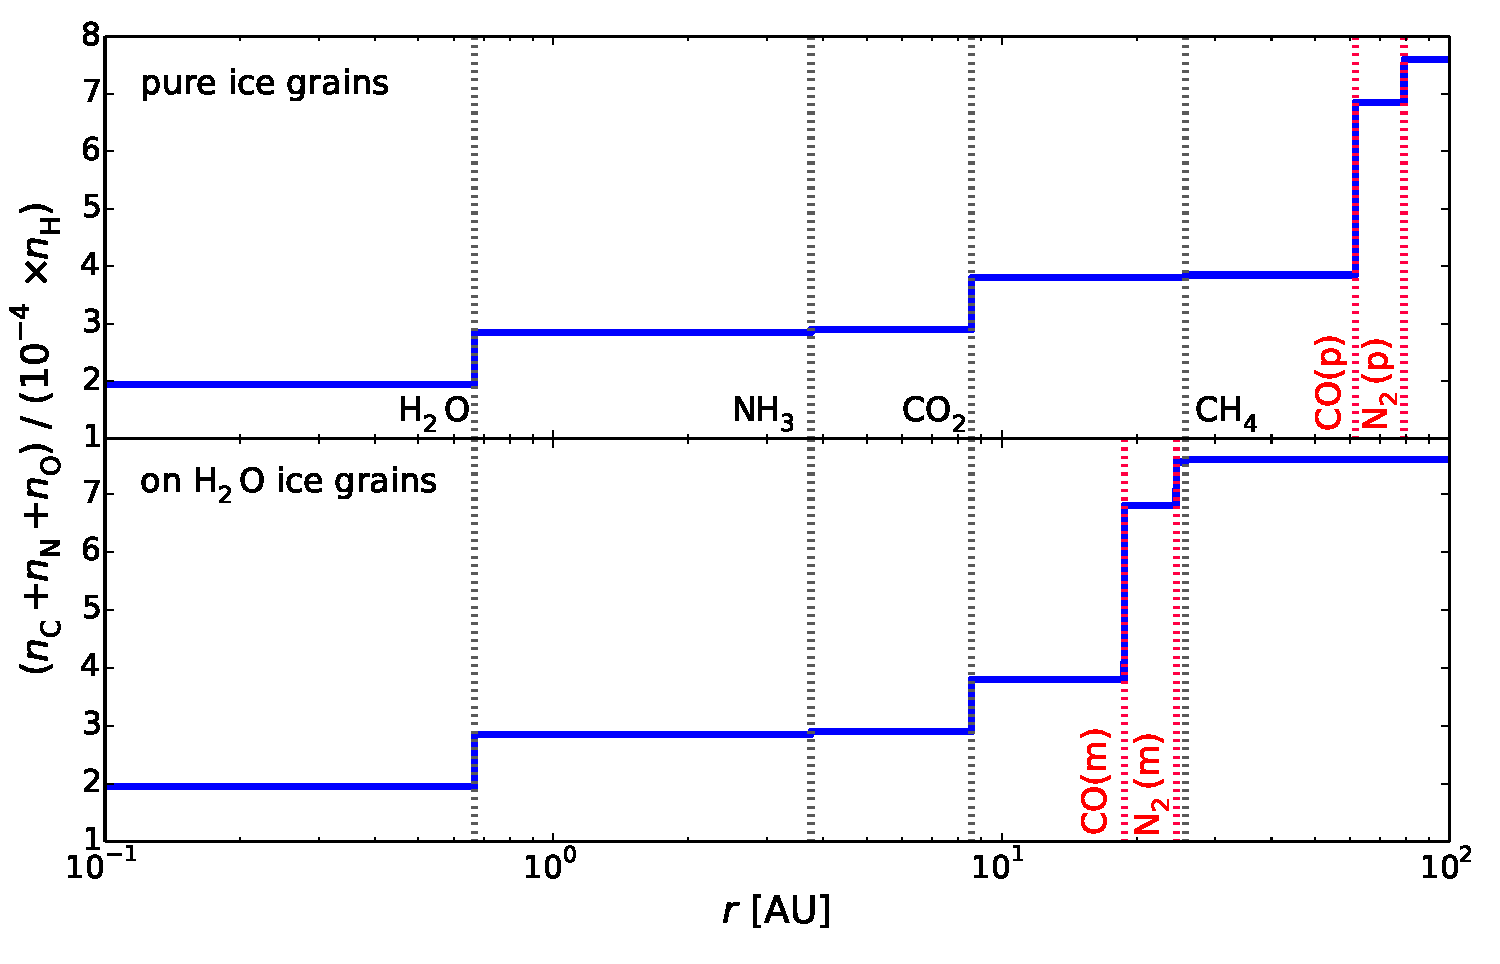
\includegraphics[width=0.95\textwidth]{figures/CNO_and_snowlines_2.pdf}
%\vspace{-0.5in}
\caption{The total carbon, nitrogen and oxygen abundance in solids as a function of semimajor axis in a static disk, for CO and N$_2$ as pure ices (top panel) and water dominated ices (bottom panel). Relevant volatile snowlines are marked by the vertical dashed lines. The grain abundances are calculated as a function of the observed median CH$_4$ and NH$_3$ abundances in protostellar cores. The total grain abundance increases with semimajor axis as more and more species freeze out.} 
\label{fig:CNOstatic}
\end{figure*}

Following \citet{chiang10} and \citet{birnstiel12}, a particle's radial drift velocity can be approximated as 
\begin{equation}
\label{eq:rdotact}
\dot{r} \approx -2 \eta \Omega_{\rm k} r \Big(\frac{\tau_{\rm s}}{1+\tau_{\rm s}^2}\Big) + \frac{\dot{r}_{\rm gas}}{1+\tau_{\rm s}^2},
\end{equation}
where the first term is the drift velocity in a non-accreting disk and the second term accounts for the radial movement of the gas. Here $\eta \approx c^2/(2 v_{\rm k}^2)$, where $v_{\rm k}$ is the Keplerian velocity, and $\tau_{\rm s} \equiv \Omega_{\rm k} t_{\rm s}$ is the dimensionless stopping time:
\begin{equation}
\label{eq:ts}
t_{\rm s}= \left\{
\begin{array}{l l}
\rho_{\rm s} s / (\rho c), & \quad s < 9 \lambda/4 \,\,\,\ \text{Epstein drag} \\
4 \rho_{\rm s} s^2 / (9 \rho c \lambda), & \quad s < 9 \lambda/4, \,\text{Re} \lesssim 1 \,\,\,\ \text{Stokes drag,}
\end{array} 
\right.
\end{equation}
where $\rho$ is the disk mid-plane density, $\lambda$ is the mean free path and Re is the Reynolds number.  The gas accretion velocity $\dot{r}_{\rm gas}$ is determined from $\dot{M}=-2 \pi r \dot{r}_{\rm gas} \Sigma$, for a fixed $\dot{M}$ and with $\Sigma$ given by Equation (\ref{eq:Sigmaact}). 

For a particle of initial size $s_0$, we solve the Equation set (\ref{eq:ddt}) with the initial conditions $s(t_0)=s_0$ and $r(t_0)=r_0$, where $t_0$ is the time at which we start the integration and $r_0$ is the particle's initial location. We stop our simulation after $t_{\rm d}=3$ Myr, the disk lifetime, since this is roughly the timescale on which planets form, and determine the desorption timescale $t_{\rm des}$ from $s(t_{\rm des})=0$, and thus a particle's desorption distance $r_{\rm des}=r(t_{\rm des})$. Our results are insensitive to our choice of $t_0$ as long as $t_0 \ll t_{\rm d}$. We note that a particle's size is initially fixed and only changes due to desorption. We thus do not take into account processes such as grain coagulation or fragmentation, which nonetheless occur in disks (e.g., \citealt{birnstiel12}, \citealt{perez12}). We discuss the effect of these processes on snowline locations in Paper I.

As we show in Paper I, a particle of initial size $s_0$ can experience three outcomes after $t_{\rm d}=3$ Myr: (1) it can remain at its initial location, (2) it can drift towards the host star, then stop without evaporating significantly, and (3) it can completely desorb on a timescale shorter than 3 Myr. Particles in scenarios (1) and (2) are thus not affected by radial drift or gas accretion, and the snowline locations are those for a static disk. In contrast, the grains in case (3) desorb practically \textit{instantaneously} and \textit{at a fixed particle-size dependent location} in the disk, regardless of their initial position. The snowline locations for these particles will thus be fixed for a given initial particle size and disk model. We have found that grains with sizes $\sim0.001$ cm $\lesssim s \lesssim$ 7 m satisfy this condition for our fiducial disk. 

%\emgr{Review disk models, desorption model, relevant timescales. State that we use a steady-state disk for the coupled drift-desorption evolution, since it is the most realistic, therefore only summarize the static and steady-state (viscous) disk. Summarize the findings of Paper I, i.e. particles of certain sizes desorb instantaneously and at a fixed particle size dependent location.}

\section{Results}
\label{sec:results}

\subsection{Snowlines in a Static Disk: The Importance of Ice Morphology}
\label{sec:snowlines}

As we note in Section \ref{sec:intro}, the disk volatile composition and the ice morphology determine the location of important snowlines. In this work we focus on the primary carbon, oxygen and nitrogen carriers, i.e. H$_2$O, CO$_2$, CO, N$_2$, and to a lesser extent, CH$_4$ and NH$_3$. %To quantify the effect of the presence of some carbon in the form of CH$_4$ and of some nitrogen in the form of NH$_3$, we use measured median CH$_4$ and NH$_3$ abundances in protostellar cores from the \textit{Spitzer} c2d Legacy ice survey \citep{evans03}. 
Our standard model is based on the median ice abundances observed toward Solar-type protostars \citep{oberg11a}, which are $n_{\rm CO_2}=0.29 \times n_{\rm H_2O}$, $n_{\rm CO}=0.38 \times n_{\rm H_2O}$, $n_{\rm CH_4}=0.0555 \times n_{\rm H_2O}$ (hereafter CH$_4$-mid) and $n_{\rm NH_3}=0.055 \times n_{\rm H_2O}$ (hereafter NH$_3$-mid). Here $n_{\rm H_2O} \approx 10^{-4} \times n_{\rm H}$ is the total water abundance \citep{vandishoeck06}, with $n_{\rm H}$ the hydrogen abundance in the disk midplane. For CO, we also take into account that the observed CO ice only traces some of the CO reservoir due to its high volatility, and similarly to \citet{oberg11} and Paper I we set the total CO abundance to $0.9 \times 10^{-4} n_{\rm H}$. Finally, we assume that all nitrogen not found in NH$_3$ is in N$_2$ and assume a Solar nitrogen abundance, $n_{\rm N}=8 \times 10^{-5} n_{\rm H}$ \citep{lodders03}. In effect, this model assumes no chemical evolution between the protostellar and disk midplane stages. This is reasonable for material that accretes onto the disk at large radii \citep{visser09}, but may overestimate the contribution of the original volatiles to the total volatile budget in the innermost disk. 

We determine the location of the H$_2$O, CO$_2$, CO, CH$_4$, N$_2$ and NH$_3$ snowlines in our static disk by balancing desorption with readsorption, following \citet{hollenbach09}. The binding energies of H$_2$O, CO$_2$, CO, CH$_4$, N$_2$ and NH$_3$ as pure ices are 5800 K, 2000 K, 834 K, 1300 K, 767 K and 2965 K, respectively (\citealt{fraser01}, \citealt{collings04}, \citealt{fayolle16}, \citealt{garrod06}, \citealt{martin14}). For CO and N$_2$ as water dominated ices, the binding energies are 1388 K and 1266 K, respectively \citep{fayolle16}. Figure \ref{fig:CNOstatic} shows the resulting snowline locations, assuming CO and N$_2$ pure ices (top panel), and CO and N$_2$ in water dominated ices (bottom panel). The ordinate displays the total carbon, oxygen and nitrogen abundance in solids as a function of the hydrogen total abundance.  As expected, the total grain abundance increases with semimajor axis, as more and more species freeze out. Freeze-out at the CO$_2$ and CO snowlines pulls more heavy elements into the grains than in the case of the H$_2$O snowline.  The CO and N$_2$ snowlines move several tens of AU inward if the ices are water dominated rather than pure. This changes the chemical abundances both in gas and dust throughout the disk, directly affecting the compositions of nascent giant planets forming in situ.

%It follows that there are several important snowlines in disks, determined both by the disk composition and ice morphology. Figure \ref{fig:CNOstatic} shows an example of the H$_2$O, CO$_2$, CO, CH$_4$, NH$_3$ and N$_2$ snowlines in a static disk, with CO and N$_2$ as pure and water dominated ices, in the top and bottom panel, respectively. 

\subsection{C/N/O Ratios in Static Disks}
\label{sec:static}

In this section we determine the C/O and N/O ratios in gas and dust throughout our static disk, and to what extent they are affected by the presence of CH$_4$ and NH$_3$ over the full range of observed CH$_4$ and NH$_3$ abundances toward low-mass protostars. In this section we only consider pure ices. %Since here we are primarily interested in the magnitude of the C/N/O ratios rather than snowline locations (which have been discussed in Section \ref{sec:snowlines}), we assume for simplicity that CO and N$_2$ are pure ices. 

We explore the parameter space of possible CH$_4$ abundances by assuming three different scenarios: (1) no CH$_4$, (2) CH$_4$-mid, and (3) the maximum CH$_4$ observed abundance (hereafter CH$_4$-max), $n_{\rm CH_4-max}=0.13 \times n_{\rm H_2O}$ \citep{oberg08}. %Similarly to Paper I, we use the H$_2$O, CO$_2$ and CO abundances of \citet{oberg11}. 
Since the abundance of carbon grains is uncertain, we assume that all the carbon that is not in the form of CH$_4$, CO and CO$_2$ is in carbon grains, so that we reproduce the Solar C/O ratio (gas+dust) of 0.54.  

Figure \ref{fig:COstatic} shows the C/O ratio in gas and dust as a function of semimajor axis in a static disk: no CH$_4$ (top panel), CH$_4$-mid (middle panel) and CH$_4$-max (bottom panel). As in \citet{oberg11} and Paper I, a gaseous C/O ratio of unity can be achieved between the CO$_2$ and CO snowlines, where oxygen gas is significantly depleted. The gas-phase C/O ratio may be further enhanced between the CO$_2$ and CH$_4$ snowlines due to the presence of additional carbon gas from CH$_4$. In this region, the C/O ratio increases by 3\% for CH$_4$-mid and by 8\% for CH$_4$-max, as displayed in the middle and bottom panels of Figure \ref{fig:COstatic}. Based on the range of observed CH$_4$ protostellar abundances, its presence in the disk only modestly affects the C/O ratio. %Given the larger uncertainties in overall volatile abundances, we can neglect CH$_4$ when estimating the C/O ratio in disks.

\begin{figure}[h!]
\centering
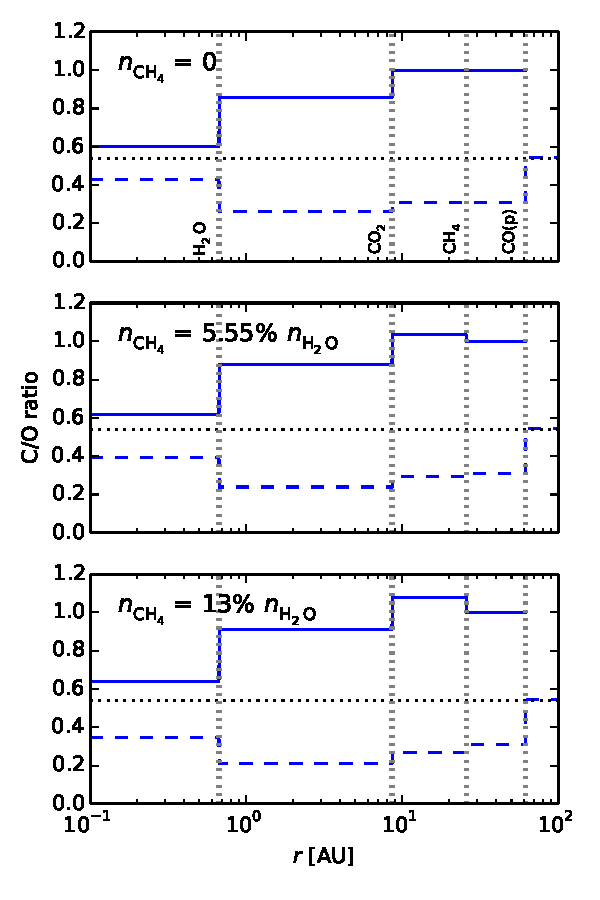
\includegraphics[width=0.5\textwidth]{figures/C_O_ratio_CH4.pdf}
%\vspace{-0.5in}
\caption{The C/O ratio in gas (solid lines) and dust (dashed lines) as a function of semimajor axis in a static disk, assuming no carbon is present in the form of CH$_4$ (top panel), the median observed CH$_4$ abundance is assumed (middle panel), and the maximum observed CH$_4$ abundance is assumed (bottom panel). The C/O estimates are performed assuming that the CO ices are in pure form. The vertical dotted lines mark the snowline locations of the main C and O carriers. The horizontal dotted lines represent the stellar C/O value. The presence of methane only modestly increases the C/O ratio in gas between the CO$_2$ and CH$_4$ snowlines.} 
\label{fig:COstatic}
\end{figure}

We assume that the main nitrogen-bearing species are N$_2$ and NH$_3$, since other volatiles that contain nitrogen have significantly lower abundances in comparison (e.g., \citealt{mumma11}). Similarly to the case of CH$_4$, we explore the parameter space of possible NH$_3$ abundances using observations toward low-mass protostars, as follows: (1) no NH$_3$, (2) NH$_3$-mid, and (3) the maximum observed NH$_3$ abundance $n_{\rm NH_3-max}=0.15 \times n_{\rm H_2O}$ \citep{bottinelli10}. In each case, the N$_2$ abundance then simply follows as $n_{\rm N_2}=(n_{\rm N}-n_{\rm NH_3})/2$. 

%Both in Solar system comets and in protoplanetary disks, carbon and oxygen are primarily contained in H$_2$O, CO$_2$ and CO (e.g., \citealt{rodgers02}, \citealt{lodders03}, \citealt{pontoppidan06}). However, some fraction of the carbon abundance may also be carried by CH$_4$ (e.g., \citealt{mumma96}), which may change the C/O ratio in gas and in dust throughout the disk. 
%To quantify the magnitude of this effect, we use measured CH$_4$ abundances in protostellar cores from the \textit{Spitzer} c2d Legacy ice survey \citep{evans03}. We explore the parameter space of possible CH$_4$ abundances by assuming three different scenarios: (1) no CH$_4$, (2) the median CH$_4$ observed abundance (hereafter CH$_4$-mid), and (3) the maximum CH$_4$ observed abundance (hereafter CH$_4$-max). Thus $n_{\rm CH_4-mid}=0.0555 \times n_{\rm H_2O}$ \citep{oberg11a} and $n_{\rm CH_4-max}=0.13 \times n_{\rm H_2O}$ \citep{oberg08}, where $n_{\rm H_2O}$ is the total H$_2$O abundance. Similarly to Paper I, we use the H$_2$O, CO$_2$ and CO abundances of \citet{oberg11}. Since the abundance of carbon grains is uncertain, we assume that all the carbon that is not in the form of CH$_4$, CO and CO$_2$ is in carbon grains, so that we reproduce the Solar C/O ratio (gas+dust) of 0.54.  

%We determine the location of the H$_2$O, CO$_2$, CO, CH$_4$, N$_2$ and NH$_3$ snowlines in our static disk by balancing desorption with readsorption, following \citet{hollenbach09}. The binding energies of H$_2$O, CO$_2$, CO, CH$_4$ and N$_2$ as pure ices are 5800 K, 2000 K, 834 K, 1300 K, respectively (\citealt{fraser01}, \citealt{collings04}, \citealt{fayolle16}, \citealt{garrod06}).





%Nitrogen is another abundant volatile in the Solar system and in disks. Chemical models of the protostellar nebula (e.g., \citealt{owen01}) and of protoplanetary disks (e.g., \citealt{rodgers02}) suggest that N$_2$ was the dominant form of nitrogen, and that giant planets have accreted their nitrogen content primarily as N$_2$ \citep{mousis14}. Observations of Solar system bodies such as Titan and Pluto show that N$_2$ is prevalent in their atmospheres (\citealt{cruikshank93}, \citealt{owen93}).  Moreover, the Rosetta spacecraft has recently made the first direct measurement of the N$_2$ abundance in comet 67P/Churyumov-Gerasimenko \citep{rubin15}. In addition to N$_2$, a fraction of the nitrogen abundances may be also carried by NH$_3$ (\citealt{bottinelli10}, \citealt{mumma11}). 

%Because of the high volatility of N$_2$, the gas phase nitrogen-to-oxygen (N/O) ratio in the outer disk
%may be even more enhanced than the C/O ratio compared to its average value in the disk. Giant planets that form at wide separations should thus have an excess of nitrogen in their atmospheres, which could be used to trace their formation origin.  
%In this study, we quantify this effect in protoplanetary disks. We assume that the main nitrogen-bearing species are N$_2$ and NH$_3$, since other volatiles that contain nitrogen have significantly lower abundances in comparison (e.g., \citealt{mumma11}). We use the measured total nitrogen abundance in the Solar system, $n_{\rm N}=8 \times 10^{-5} n_{\rm H}$ \citep{lodders03}, where $n_{\rm H}$ is the hydrogen abundance in the disk midplane. Similarly to the case of CH$_4$ (see Section \ref{sec:CH4}), we explore the parameter space of possible NH$_3$ abundances using data from the Spitzer c2d Legacy ice survey, as follows: (1) no NH$_3$, (2) the median NH$_3$ observed abundance $n_{\rm NH_3-mid}=0.055 \times n_{\rm H_2O}$ \citep{oberg11a}, and (3) the maximum observed NH$_3$ abundance $n_{\rm NH_3-max}=0.1537 \times n_{\rm H_2O}$ \citep{bottinelli10}. In each case, the N$_2$ abundance then simply follows as $n_{\rm N_2}=(n_{\rm N}-n_{\rm NH_3})/2$. We determine the locations of the N$_2$ and NH$_3$ snowlines by balancing desorption with readsorption \citep{hollenbach09}, with N$_2$ and NH$_3$ pure ice binding energies of  767 K and  2965 K, respectively (\citealt{fayolle16}, \citealt{martin14}). 

\begin{figure}[h!]
\centering
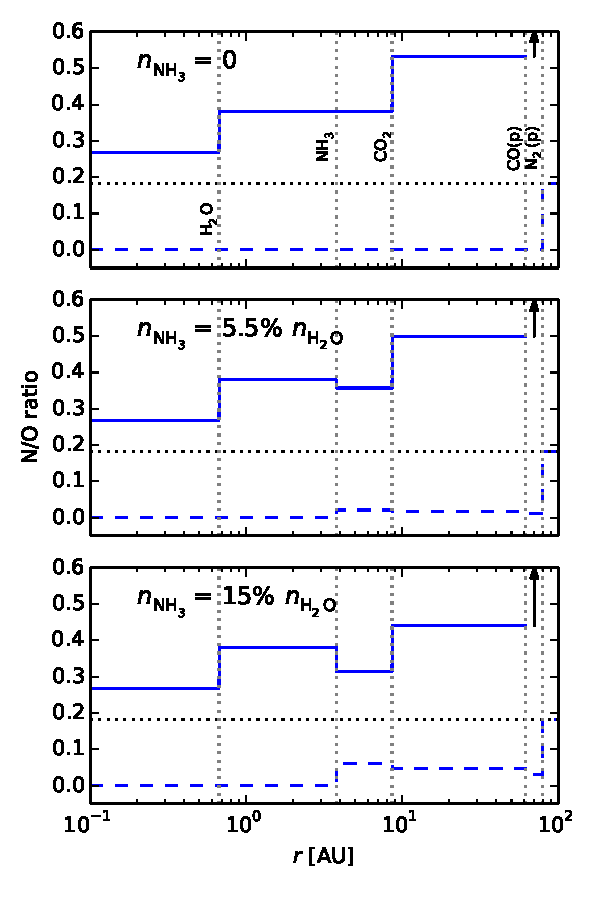
\includegraphics[width=0.5\textwidth]{figures/N_O_ratio.pdf}
%\vspace{-0.5in}
\caption{The N/O ratio in gas (solid lines) and dust (dashed lines) as a function of semimajor axis in a static disk, assuming no nitrogen is present in the form of NH$_3$ (top panel), the median observed NH$_3$ abundance is assumed (middle panel), and the maximum observed NH$_3$ abundance is assumed (bottom panel). The N/O estimates are performed assuming that the CO and N$_2$ ices are in pure form. The vertical dotted lines mark the snowline locations of the main C,O and N carriers. The horizontal dotted lines represent the average N/O value in the disk. The gas-phase N/O ratio is enhanced by a factor of two between the H$_2$O and CO$_2$ snowlines compared to its average value, and by a factor of three between the CO$_2$ and CO snowlines. The arrows mark a highly elevated N/O ratio in gas between the CO and N$_2$ snowlines due to the depletion of oxygen gas in this region. The presence of NH$_3$ moderately decreases the N/O ratio in gas between the NH$_3$ and CO$_2$ snowlines.} 
\label{fig:Nstatic}
\end{figure}

Figure \ref{fig:Nstatic} shows the snowline locations of the main oxygen and nitrogen carriers and the N/O ratio in gas and dust as a function of semimajor axis in a static disk, for our three choices of the NH$_3$ abundance: no NH$_3$ (top panel), NH$_3$-mid (middle panel) and NH$_3$-max (bottom panel). For comparison, the horizontal dotted lines show the average N/O ratio in the disk. As expected, the gaseous N/O ratio generally exhibits an increasing trend towards the outer disk as more oxygen gas is depleted, with small decreases between the NH$_3$ and CO$_2$ snowlines (by 6\% for NH$_3$-mid and by 18\% for NH$_3$-max, respectively) due to NH$_3$ freeze-out. While the presence of NH$_3$ only moderately affects our results for the N/O ratio, NH$_3$ is important since otherwise the nitrogen content in solid bodies would be more depleted than is observed for comets and asteroids (\citealt{wyckoff91}, \citealt{mumma11}, \citealt{bergin15}).

The gas-phase N/O ratio is enhanced by a factor of two outside the H$_2$O snowline compared to its average value, by more than a factor of three between the CO$_2$ and CO snowlines, and by orders of magnitude between the CO and N$_2$ snowlines. This latter region can span tens of AU depending on disk parameters and the relative CO and N$_2$ ice binding environment. This N/O  enhancement is more pronounced than the C/O gas phase enhancement of a factor of two in the outer disk (see Figure \ref{fig:COstatic}). %The N/O ratio reaches particularly high values between the CO and N$_2$ snowlines, where all the oxygen is now contained in grains. 

\subsection{C/N/O Ratios in Dynamic Disks}
\label{sec:dynamic}

%As noted in Section \ref{sec:intro}, the CO binding energy varies significantly depending on the morphology of the icy grains. If CO ice is in a water dominated environment, its binding energy will be larger than in the pure ice case (834 K) due to the higher binding energy of CO to H$_2$O than to other CO molecules. \citet{fayolle16} find a CO binding energy of 1388 K in the water dominated ice scenario. 


Here we use the model of Section \ref{sec:review} to estimate the movement of the CO and N$_2$ snowlines for different grain morphologies in a viscous disk. Figure \ref{fig:CO_ratio} shows the H$_2$O, CO$_2$ and CO snowline locations for particles with initial sizes $\sim0.05$ cm $\lesssim s \lesssim$ 7 m as well as estimates for the C/O ratio in gas and dust in a viscous disk, with the CO snowline calculated under different grain morphologies as noted above. We assume there is no carbon in the form of CH$_4$. The true snowline for particles that desorb outside the static snowline is the static snowline itself, hence desorbing particles with $s<0.05$ cm do not form true snowlines. If the CO binding environment is known, the CO snowline moves inward by up to $\sim$50 \% compared to a static disk for each case (pure and water dominated ices) due to disk dynamics. The full range of potential CO snowlines taking into account both ice morphology and disk dynamics span $\sim$8.7 AU to $\sim$61 AU, which is a factor of $\sim$7 difference. This implies that gas phase C/O ratios of order unity may be reached in the giant planet forming zone, and the CO snowline may be inside 10 AU for certain disk parameters.  

\begin{figure}[h!]
\centering
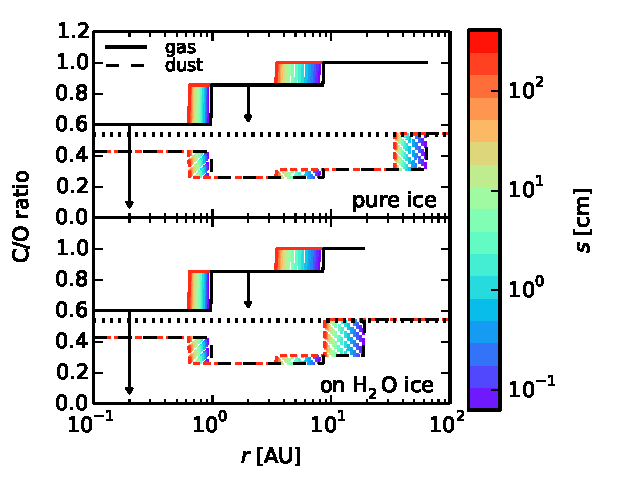
\includegraphics[width=0.5\textwidth]{figures/C_O_water_ice.pdf}
%\vspace{-0.5in}
\caption{C/O ratio estimates in gas (solid lines) and dust (dashed lines) as function of semimajor axis in a viscous disk, for CO as pure ice (top panel) or as water dominated ices (bottom panel). The H$_2$O, CO$_2$ and CO snowlines are shown for particles with initial sizes $\sim0.05$ cm $\lesssim s \lesssim$ 7 m as indicated by the color bar. The C/O ratio in a static disk (black lines) is shown for comparison. The arrows show that the C/O ratio in gas will decrease inside the H$_2$O and CO$_2$
snowlines in the viscous disk, as the relative fluxes of the desorbed icy
particles and the overall nebular gas will cause an excess of oxygen gas inside these snowlines (see Paper I for details). The presence of CO in a water ice environment rather than as pure ice moves the CO snowline significantly inward by $\sim$70\%. Taken together, disk dynamics and ice morphology move the CO snowline inward by a factor of $\sim$7.} 
\label{fig:CO_ratio}
\end{figure}

%As in the case for CO, the N$_2$ binding energy is also strongly dependent on the ice environment in which the grain resides. If N$_2$ is a water dominated ice, the N$_2$ binding energy is 1266 K \citep{fayolle16}. 

Figure \ref{fig:NO_ratio} shows the H$_2$O, CO$_2$, CO and N$_2$ snowline locations in a viscous disk for the same range of initial particle sizes as in Figure \ref{fig:CO_ratio}, and with the CO and N$_2$ snowlines calculated assuming different grain morphologies as explained above, as well as estimates for the N/O ratio throughout the disk. For simplicity, we assume that all nitrogen is the form of N$_2$. This choice is justified since the presence of some NH$_3$ only moderately changes the N/O ratio (see Figure \ref{fig:Nstatic}), and since we are primarily interested in the N$_2$ snowline locations rather than exact values for the N/O ratio. The innermost N$_2$ snowlines in the viscous disk, created by particles with $s \sim 7$ m for our fiducial model, are located at $r_{\rm N_2, pure} \approx 42$ AU for N$_2$ as pure ice and at $r_{\rm N_2, water} \approx 11$ AU for N$_2$ in water dominated ices. Thus for each case (pure versus water dominated ices), the N$_2$ snowline moves inward by up to 50\% due to disk dynamics. By taking into account both ice morphology and disk dynamics, the full range of potential N$_2$ snowlines span $\sim$11 to $\sim$79 AU, which is a factor of $\sim$7 difference. Similarly to the case for CO, the N$_2$ snowline may be close to 10 AU for certain disk models. 


\begin{figure}[h!]
\centering
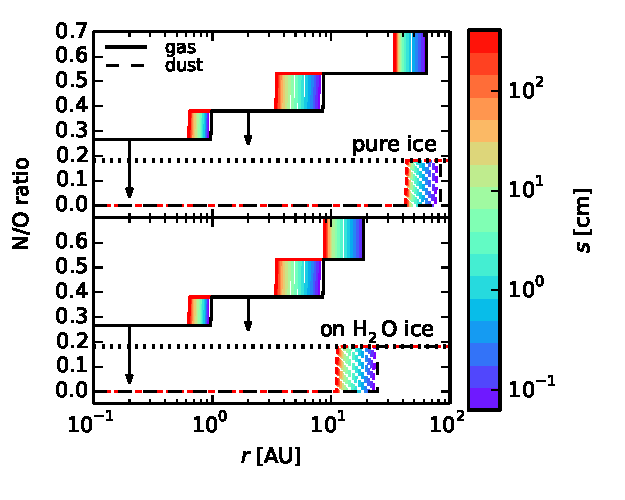
\includegraphics[width=0.5\textwidth]{figures/N_O_water_ice_many.pdf}
%\vspace{-0.5in}
\caption{N/O ratio estimates in gas (solid lines) and dust (dashed lines) as function of semimajor axis in a viscous disk, for CO and N$_2$ as pure ices (top panel) or as water dominated ices (bottom panel). The H$_2$O, CO$_2$, CO and N$_2$ snowlines are shown for particles with initial sizes $\sim0.05$ cm $\lesssim s \lesssim$ 7 m as indicated by the color bar. The N/O ratio in a static disk (black lines) is shown for comparison. The arrows show that the N/O ratio in gas will decrease inside the H$_2$O and CO$_2$ snowlines in the viscous disk, as the relative fluxes of the desorbed icy
particles and the overall nebular gas will cause an excess of oxygen gas inside these snowlines (see Paper I for details). Radial drift and gas accretion move the N$_2$ snowline inward by up to $\sim$50\% compared to a static disk. The presence of N$_2$ in a water ice environment rather than as pure ice moves the N$_2$ snowline significantly inward by $\sim$70\%. Taken together, disk dynamics and ice morphology move the N$_2$ snowline inward by a factor of $\sim$7. The results of an enhanced gas-phase N/O ratio between the H$_2$O and CO snowlines compared to its average value, and of highly elevated N/O ratios in gas between the CO and N$_2$ snowlines (see Figure \ref{fig:Nstatic}), are preserved.}  
\label{fig:NO_ratio}
\end{figure}



%Our results for the N/O ratio imply that both gas phase and solid nitrogen abundances are enhanced in the outer disk, and that the regions in which these enhancements occur depend on disk dynamics and particle morphology. 


\section{Discussion}
\label{sec:discussion}

%\emgr{Discuss how entrapment of volatiles by H2O affects volatile abundances and C/O ratios. Re-emphasize the fact that the C/O and N/O ratios are upper estimates, and that CH4 and NH3 might matter in a viscous disk. State that we plan to address this in a future paper. More TBD.}
This study shows that the gas-phase N/O ratio in protoplanetary disks is considerably enhanced throughout most of the disk midplane compared to its average value. As demonstrated in Figure \ref{fig:enhance}, the gaseous N/O ratio is enhanced by a factor of two beyond the H$_2$O snowline, by more than a factor of three between the CO$_2$ and CO snowlines, and by several orders of magnitude between the CO and N$_2$ snowlines. Thus constraining the N/O ratio in a giant planet atmosphere could be used to trace its formation origins. 

Theoretical models of the magnitude and role of N/O (and N/C) ratios in exoplanet atmospheres are needed in order to use these ratios as probes for a planet's formation location. Models that explore the effect of varying the C/O ratio in exoplanet atmospheres exist in literature, and they display a large and observable effect on gas giant envelope chemistry (\citealt{lodders09}, \citealt{molliere15}). However, no similar model explorations exist for the effect of N/O and C/N/O ratios, and both are needed to exploit this potential constraint. Given the existence of such theoretical models, measurements of the N/O ratio in planetary envelopes may be possible to infer from atmospheric compositions of nitrogen versus carbon and oxygen bearing species. Nitrogen carriers have not been targeted so far due to lack of instrument sensitivity, but such observations and detections are likely in the near future with the advent of JWST (e.g., NH$_3$, \citealt{greene16}). The N/O ratio enhancement is larger than that of the gas phase C/O ratio throughout most of the disk. Thus measurements of an enhanced C/O ratio in an exoplanet atmosphere could be corroborated (disproved) by measurements of enhanced (non-enhanced) N/O ratios. Moreover, Figure \ref{fig:enhance} shows that giant planets that have formed in situ between the H$_2$O and CO snowlines are expected to present elevated both C/O and N/O ratios in their atmospheres, whereas planets between the CO and N$_2$ snowlines will have a highly enhanced N/O ratio in their atmospheres, but not C/O.  

\begin{figure}[h!]
\centering
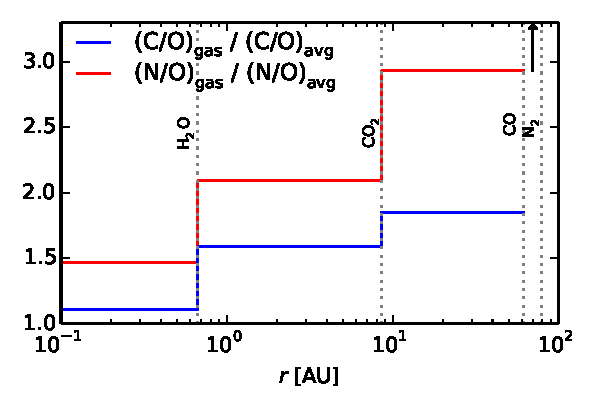
\includegraphics[width=0.5\textwidth]{figures/CN_norm.pdf}
%\vspace{-0.5in}
\caption{Gas phase C/O (blue curve) and N/O (red curve) ratios divided by the average C/O and N/O ratio in a static disk, assuming CO and N$_2$ are pure ices, and there is no CH$_4$ or NH$_3$. The dashed vertical lines mark the H$_2$O, CO$_2$, CO and N$_2$ snowlines. The arrow indicates that the N/O ratio is enhanced by orders of magnitude compared to its average value between the CO and N$_2$ snowlines. The gaseous N/O ratio is enhanced throughout most of the disk, and more enhanced than the C/O ratio.}  
\label{fig:enhance}
\end{figure}




Due to disk dynamics and ice morphology, the locations of the CO and N$_2$ snowlines, and thus the disk regions with highly elevated gas phase N/O and C/O ratios, are uncertain and may span tens of AU. Both ice morphologies discussed in this study, pure and water dominated ices, are plausible in protoplanetary disks and depend on whether H$_2$O and CO ices formed on similar timescales or successively (e.g., \citealt{garrod11}). Observations of protostellar cores show that a large fraction of CO is bound in a pure ice multilayer \citep{pontoppidan03}, but theoretical models also suggest an icy mantle structure where CO resides on a H$_2$O ice layer (e.g., \citealt{collings03}). One can also imagine a scenario where CO is in a water binding environment and N$_2$ is not. This could be attributed to the fact that H$_2$O may bind preferentially to CO than N$_2$, since both H$_2$O and CO are polar molecules while N$_2$ is not. It is also possible for N$_2$ ices to form later than CO (e.g., \citealt{pagani12}), and thus be deposited on the outer layers of the icy mantles which are typically water poor (e.g., \citealt{garrod11}). The impact of the ice environment on the snowline location is much smaller in the case of CO$_2$ and NH$_3$, as their binding energies and behavior are closer to that of H$_2$O. No detailed measurements for the CH$_4$ binding energy in a water environment exist so far, but due to its low desorption temperature a similar behavior to that of CO and N$_2$ would be expected. While the presence of some carbon in the form of CH$_4$ only modestly affects our results, CH$_4$ may become important in disks where a large fraction of the CO abundance has been converted into hydrocarbons (e.g., \citealt{du15}). 

Changes in stellar luminosity (e.g., \citealt{kennedy06}) and gas mass accretion rate (e.g., \citealt{chambers09}), as well as the evolution of icy dust particles due to grain growth and fragmentation (e.g., \citealt{birnstiel12}), may introduce additional uncertainties in the snowline locations, and thus the C/N/O ratios. Given the number of uncertainties in snowline locations, detections of snowlines in a sample of disks at different evolutionary stages are needed to provide observational constraints on the relative importance of ice morphology and disk dynamics in setting snowline locations. The uncertainties in snowline locations caused by disk dynamics, ice morphology, and other effects outlined above can be resolved in extreme cases, such as a detection of a CO snowline at a temperature corresponding to pure CO ice desorption in a static disk (e.g., \citealt{qi13} at $\sim$ 17 K) or CO desorption from a water dominated ice in a dynamic disk. In intermediate cases it is more difficult to resolve the relative importance of ice morphology and disk dynamics. For example, the CO snowline in HD 163296 is at a higher temperature of $\sim$ 25 K \citep{qi15}, which could be caused either by CO being in a water dominated environment or by dynamical effects that push the CO snowline inward. Detections of multiple snowlines in the same disk could potentially break this degeneracy. %, since CO and N$_2$ desorb at substantially different temperatures, and therefore locations, if the former is water dominated and the latter is in a pure ice environment. 

%Current detections include the H$_2$O snowline in TW Hya \citep{zhang13} and the CO snowline in TW Hya \citep{qi13} and HD 163296 \citep{qi15}. More snowline detections in disks of different ages are expected in future ALMA cycles.  Snowline observations may also be used to constrain the degree of turbulence in protoplanetary disks \citep{owen14}. We note, however, that observations of snowlines may not be enough to break the degeneracies in snowline locations produced by disk dynamics, ice morphology, and other effects outlined above. For example, a detection of the CO snowline at a temperature higher than the assumed desorption temperature in a static disk with CO as pure ice ($\sim$17 K, e.g. \citealt{qi13}) could be caused either by CO being in a water dominated environment or by dynamical effects that push the CO snowline inward. This degeneracy can be broken in extreme cases --- for our fiducial disk model, this implies a detection of a CO snowline close to $\sim$9 AU or $\sim$61 AU (see Section \ref{sec:dynamic}). 


 %The impact of the ice environment on the snowline location is much smaller in the case of CO$_2$ and NH$_3$, as their binding energies and behavior are closer to that of H$_2$O. No detailed measurements for the CH$_4$ binding energy in a water environment exist so far, but due to its low desorption temperature a similar behavior to that of CO and N$_2$ would be expected. While the presence of some carbon in the form of CH$_4$ only modestly affects our results, CH$_4$ may become important in disks where a large fraction of the CO abundance has been converted into hydrocarbons (e.g., \citealt{du15}).   %It is thus crucial to build a quantitative framework to explore the range of snowline locations and thus gaseous C/N/O ratios across disks with different dynamics and grain morphologies, as such models are currently lacking. %The theoretical expectations for N/O ratios in disks and giant planets may be further constrained by future JWST observations of exoplanet atmospheric spectra and detections of nitrogen bearing species (e.g., NH$_3$, \citealt{greene16}).   

Uncertainties in snowline locations of this magnitude also affect interpretations of Solar system observations. Recent measurements of nitrogen abundance in comet 67P/Churyumov-Gerasimenko found a N$_2$/CO ratio $\sim 10^{-3}$ \citep{rubin15}. A low N$_2$/CO ratio is consistent with comets having formed inside the N$_2$ snowline where N$_2$ is still in the gas phase. Theoretical models suggest that Jupiter-family comets, such as 67P, originate from the Kuiper belt (\citealt{duncan97}; but see \citealt{rubin15} for alternative formation scenarios for 67P). It is thus possible, in principle, to use measurements of the N$_2$ abundance in Jupiter-family comets to determine where the N$_2$ snowline was located in our Solar system. However due to the uncertainty in the calculated location of the N$_2$ snowline (see Section \ref{sec:dynamic}), more detailed modeling is needed. 

%Finally, detections of snowlines in disks that are reasonably well characterized could help further constrain the dynamics and ice morphology in the disks.    


\section{Summary}
\label{sec:summary}

In this paper we explore the role of icy grain morphology and disk dynamics on the snowline locations of major volatile carrier molecules and the C/N/O ratios in protoplanetary disks. We enhance the coupled drift-desorption model developed in \citet{piso15b} by adding more carbon- and nitrogen-bearing species into our framework, and by considering different binding ice environments. Our results can be summarized as follows:

\begin{enumerate}

\item Due to the high volatility of N$_2$, the gaseous N/O ratio outside the H$_2$O snowline is enhanced by a factor of two compared to its average value, by more than a factor of three between the CO$_2$ and CO snowlines, and by many orders of magnitude between the CO and N$_2$ snowlines due to the complete depletion of oxygen gas in this region. This enhancement is more pronounced than in the case of the gas-phase C/O ratio, which is increased by at most a factor of two compared to the stellar value. %Moreover, the N/O ratio in gas is expected to be very large between the CO and N$_2$ snowlines due to the complete depletion of oxygen gas in this region

\item The effect of CH$_4$ and NH$_3$ on the C/O and N/O ratios is small, even when we consider the maximum observed CH$_4$ and NH$_3$ abundances in protostellar cores. In this scenario, the gas phase C/O ratio increases by 8\% between the CO$_2$ and CH$_4$ snowlines, and  the gaseous N/O ratio decreases by 18\% between the NH$_3$ and CO$_2$ snowlines. In both cases, large gas phase C/O and N/O ratios in the outer disk are preserved.

\item Grain composition sensitively affects the CO and N$_2$ snowline locations. If CO and N$_2$ reside in water dominated rather than pure ices, their snowlines move inward by up to $\sim$70 \%. This effect is separate from that of radial drift and viscous gas accretion, which also cause an inward movement of the CO and N$_2$ snowlines by up to $\sim$50 \%. 

\item The locations of the CO and N$_2$ snowlines are uncertain when we consider both viscous versus static disks, and pure versus water dominated ices. The snowlines in a viscous disk with CO or N$_2$ in a water environment are by up to a factor of $\sim$7 closer to the host star that in a static disk with CO or N$_2$ as pure ices. 

\end{enumerate}

Our results have direct consequences for the composition of nascent giant planets. The considerable inward movement of the CO and N$_2$ snowlines due to the ice grains being water dominated rather than pure ices implies than giant planets with high C/O and/or N/O ratios in their atmospheres may form closer in than previously predicted by theoretical models. Moreover, our model shows that wide separation gas giants may have an excess of nitrogen in their envelopes, which may be used to trace their origins. %In future work, we plan to add new levels of complexity to our model in terms of disk chemistry, dynamics, and planetary dynamics, thus forming a solid framework for understanding the origins of gas giants. 
\chapter{Summary and Future Directions}
\label{conclusion}

In this thesis, we have calculated the minimum core mass required to form wide-separation gas giants at different disk locations, and for different equations of state of the nebular gas and dust opacities. We have also determined how disk dynamics and volatile abundance and morphology affect volatile snowline locations, the C/N/O ratios across the disk, and therefore the compositions of nascent giant planets. Our results are summarized in Sections \ref{sec:core} and \ref{sec:volatile}, and we present directions for future work in Section \ref{sec:future}. 

\section{Minimum Core Masses for Giant Planet Formation}
\label{sec:core}

In Chapters 2 and 3, we determined the minimum core mass $M_{\rm crit}$ required to form a gas giant at distances between 5 and 100 AU from the host star, motivated by the fact that standard core accretion models cannot explain the formation of giant planets in the outer disk. This minimum applies when the solid cores are no longer accreting solids, since any additional heating due to planetesimal accretion would heat up the core's atmosphere, inhibit its ability to cool and contract, and therefore increase the critical core mass. We thus considered atmospheres accreting around fully formed cores and undergoing Kelvin-Helmholtz contraction. In Chapter 2, we developed a quasi-static atmospheric evolution model by generating a series of static atmospheric profiles that are then connected temporally through a cooling equation. We considered an envelope structure consisting of an inner convective region and an outer radiative layer, and assumed a constant luminosity in the outer radiative region. We demonstrated that this is a valid approximation for our parameter space of interest. For an ideal gas polytrope and standard interstellar (ISM) opacities, we have found that $M_{\rm crit}$ decreases with semimajor axis from $\sim 8.5 M_{\oplus}$ at 5 AU to $\sim 3.5 M_{\oplus}$ at 100 AU. Our results are lower than the typically quoted value of $M_{\rm crit} \sim 10 M_{\oplus}$ (e.g., \citealt{rafikov06}), even in the more inner parts of the disk. 

To obtain more robust quantitative results, in Chapter 3 we expanded the model developed in Chapter 2 by considering a realistic equation of state (EOS) for the nebular gas and realistic dust opacities that take into account grain growth. We parametrized the EOS through the adiabatic gradient $\delad$ (defined in Chapter 2), as $\delad$ relates the gas pressure, temperature and density. While for an ideal gas EOS $\delad$ is constant, non-ideal EOS effects cause features in the adiabatic gradient that change the atmospheric structure. At high temperatures, molecular hydrogen dissociates, while at low-temperatures the rotational states of the hydrogen molecule are only partially excited so it no longer behaves like an ideal gas, due to the existence of H$_2$ in two spin isomeric forms, ortho- and parahydrogen. Both of these effects increase $M_{\rm crit}$ by a factor of $\sim$2 compared to the ideal gas. In contrast, grain growth opacities decrease $M_{\rm crit}$ dramatically. By taking these two competing effects together, we calculate $M_{\rm crit} \sim 8 M_{\oplus}$ at 5 AU, decreasing to $\sim 5 M_{\oplus}$ at 100 AU. While our atmospheric model is not equipped to calculate the critical core mass when grain coagulation is taken into account, we have demonstrated that grain growth with coagulation may decrease $M_{\rm crit}$ by up to one order of magnitude; $M_{\rm crit}$ may be as low as 1 $M_{\oplus}$. Our study thus clearly challenges previous claims that core accretion cannot operate in the outer disk, reopening the case for in situ formation of wide separation gas giants. 

\section{The Role of Disk Dynamics and Ice Morphology on Snowline Locations and the C/N/O Ratios}
\label{sec:volatile}

In Chapters 4 and 5, we determined the effect of disk dynamics and ice morphology on the C/N/O ratio in active disks, which has direct implications on gas giant compositions. This study was motivated by the fact that the locations of volatile snowlines in protoplanetary disks are a defining feature of both gas giant and disk chemistry, as they provide vital information about the abundance of these molecules in gas and dust throughout the disk. In Chapter 4, we expanded the model of \citet{oberg11} by considering the effect of disk dynamics on the snowline locations of the main carbon and oxygen carriers, i.e. H$_2$O, CO$_2$ and CO, and thus on the C/O ratio in dust and gas throughout the disk. We studied the effect of radial drift of solids and viscous gas accretion onto the central star on snowline locations by developing a semi-analytical model, which we applied to three different disks in increasing order of complexity. We applied our model for a range of initial particle sizes and calculated how drift and gas accretion affect their desorption location. We have found that there is a range of particle sizes, $0.05$ cm $\lesssim s \lesssim$ 7 m for our particular parameters, that desorb almost instantaneously and at a fixed particle-size dependent location from the central star, regardless of their initial position. Based on this information, we calculated the H$_2$O, CO$_2$ and CO snowline locations for different particle sizes in this range, and made estimates for the C/O ratio throughout the disk. We have found that the snowlines move inward as the particle size increases, and may differ by up to a factor of $\sim$2 due to drift and gas accretion compared to a static disk, which does not experience any dynamical processes. This variation in snowline locations is significant, and has important consequences for the compositions of gas giants forming in situ. 

In Chapter 5, we expanded the model developed in Chapter 4 by considering additional volatiles, chemical abundances, and ice morphologies. As nitrogen is highly abundant in the Solar System and primarily found as N$_2$, we added nitrogen bearing species such as N$_2$ and NH$_3$ to our model, as well as hydrocarbons (specifically, CH$_4$). Motivated by laboratory experiments (e.g., \citealt{fayolle16}) that find significantly different binding energies for CO and N$_2$ depending on the ice environment in which they reside (pure versus water dominated ices), we calculated the CO and N$_2$ snowlines for both scenarios. We calculated the N/O ratio in static disks and found that it is highly enhanced compared to the stellar value: by a factor of $\sim$2 between the H$_2$O and CO$_2$ snowlines, by more than a factor of 3 between the CO$_2$ and CO snowlines, and by many orders of magnitude between the CO and N$_2$ snowlines, where oxygen gas is depleted. Thus we expect wide-separation giants to have an excess of nitrogen in their atmospheres, which may be used to trace their formation origins. We have also found that the binding environment has a large effect on the CO and N$_2$ snowline locations and may change them by factors of 3-4, both for static and dynamic disks. Thus by considering the combined effect of disk dynamics and ice morphology, the CO and N$_2$ snowline locations may change by up to a factor of $\sim$7, and may span 11-79 AU for N$_2$ in our disk model. This large uncertainty in snowline locations means that observations that anchor snowline locations at different stages of planet
formation are key to develop C/N/O ratios as a probe of planet formation zones. 

\section{Future Directions}
\label{sec:future}

Our work has made important strides in our understudying of disk and planet compositions and the tight link between the two, as well as the effect of disk dynamics and chemistry on disk and planet compositions. As a first step, we plan to expand this work by considering the effect of diffusion on the C/N/O ratios in viscous steady-state disks. Similarly to the model of \citet{owen14}, we will develop a simplified method to estimate the abundance of different volatiles at various disk locations, and thus their effect on the C/N/O ratio both in static and dynamic disks. 

Through analytical and numerical calculations, we will explore a range of dynamical processes that may affect snowline locations and the distribution of volatiles in disks, expanding and generalizing the framework developed in Chapter 4 and 5. Such effects include particle growth and fragmentation, as well as variations in the gas mass accretion rate and stellar luminosity.

The complexity of disk chemistry means that coupling it with dynamical processes, while necessary, is non-trivial. As a next step we will thus couple the dynamical framework outlined above with time-dependent chemical models of increasing complexity, informed by results from state-of-the-art disk chemistry models (that can only be run on static disks).  By having a better understudying on how disk chemistry and dynamics affect the composition of nascent, and eventually mature planets, our work may provide essential context for characterizing the gas giants
that instruments such as JWST and the TESS will one day discover.  
 

\begin{appendices}
    \chapter{Derivation of the Global Energy Equation}
\label{sec:globalderiv}

%\section{Derivation of the Global Energy Equation}\label{sec:globalderiv}

To derive  the global energy equation (\ref{1eq:coolingglobal}) for an embedded protoplanet, we generalize the analogous calculations in stellar structure theory, e.g.\ in \S4.3 of \citet{kippenhahn90}.  For our problem, we add the effects of finite core radius, surface pressure and mass accretion. We start with the local energy equation (\ref{1eq:structd}), whose more natural form in Lagrangian (mass) coordinates is $\p L/ \p m = \epsilon - T \p S /\p t$.  Integrating from the core to a higher shell with enclosed mass $M$ gives:
\begin{subeqnarray}
L - L\co &=& \int_{M\co}^M {\p L \over \p m} dm \\
&=& \int_{M\co}^M \left(\epsilon - T {\p S \over \p t} \right)dm \\
&=& \Gamma  - \int_{M\co}^M{\p u \over \p t} dm +  \int_{M\co}^M {P \over \rho^2} {\p \rho \over \p t} dm\slabel{eq:DLc}\, ,
\end{subeqnarray} 
with $\Gamma = \int \epsilon dm$ the integral of the direct heating rate, and applying the first law of thermodynamics in the final step.

The global energy equation is derived by eliminating the partial time derivatives in \Eq{eq:DLc}, which are performed at a fixed mass,
in favor of total time derivatives, denoted with overdots.  %The physical distinction is that total derivatives include mass  accreted through the outer boundary.  
For instance, the surface radius $R$ of the shell with enclosed mass $M$ evolves as  
\begin{equation}\label{eq:Rdot}
 \dot{R} = {\p R \over \p t} + {\dot{M} \over 4 \pi R^2 \rho_M},
\end{equation} 
where $\p R/\p t$ gives the Lagrangian contraction of the ``original" shell, and mass accretion through the upper boundary at rate $\dot{M}$ also changes the shell location.  
%The subscript $M$  denotes quantities at the upper boundary of total mass $M$ (though it is omitted from $M$ and $R$).  
Similarly, the volume $V = (4 \pi/3)R^3$ and pressure at the outer shell evolve as
\begin{subeqnarray}\label{eq:dot}
\dot{V}_M &=&  {\p V_{\rm M} \over \p t} + {\dot{M} \over \rho_{\rm M}}  \\
 \dot{P}_M &=& {\p P_{\rm M} \over \p t} + {\p P_M \over \p m}\dot{M} =  {\p P_{\rm M} \over \p t} - {G M  \over 4 \pi R^4} \dot{M}\, .
\end{subeqnarray} 
This derivation holds the core mass and radius fixed, $\dot{M}\co = \dot{R}\co = 0$.  Therefore, the core pressure satisfies
\begin{equation}\label{eq:Pcdot}
 \dot{P}\co = \p P\co / \p t \, .
\end{equation}
The internal energy integral follows simply from  Leibniz's rule as
\begin{equation}\label{eq:udot}
\int_{M\co}^{M(t)}{\p u \over \p t} dm = \dot{U}  -  \dot{M}u_M\, .
\end{equation} 
To make further progress, we use the virial theorem:
\begin{equation}
\label{eq:virial}
E_G=-3 \int_{M\co}^M \frac{P}{\rho} dm + 4 \pi (R^3 P_M-R\co^3 P\co),
\end{equation}
which follows from \Eqsss{1eq:structb}{1eq:structa}{1eq:Eg} by integrating hydrostatic balance in Lagrangian coordinates.  As an aside, the integral in equation (\ref{eq:virial}) can be evaluated for a polytropic EOS to give simple expressions for the total energy:
\begin{subeqnarray}
E&=&(1-\zeta)U+4 \pi (R^3 P_M-R\co^3 P\co) \slabel{eq:vira} \\
&=&\frac{\zeta-1}{\zeta}E_G+\frac{4 \pi}{\zeta} (R^3 P_M-R\co^3 P\co) \slabel{eq:virb} \, ,
\end{subeqnarray}
where $\zeta \equiv 3(\gamma - 1)$.  We will not make this assumption and will keep the EOS general.

To express the work integral, i.e. the final term in \Eq{eq:DLc}, in terms of changes to gravitational energy, we first take the
 time derivative of \Eq{eq:virial}:
\begin{eqnarray}\label{eq:EGdot}
\dot{E}_G = 3  \int_{M\co}^M {P \over \rho^2} {\p \rho \over \p t} dm -3 \int_{M\co}^M {\p P\over \p t}{dm \over \rho} 
 -  3{P_M \over \rho_M} \dot{M}+ 3 \dot{P}_M V_M -3 \dot{P}\co V\co  + 3  P_M {\dot{ V}_M} \, . 
\end{eqnarray} 
%where the volumes, $V_M = 4 \pi R^3/3$ and $V\co = 4 \pi R\co^3/3$. 
The first integral in \Eq{eq:EGdot} is the one we want, but the second one must be eliminated.  The time derivative of \Eq{1eq:Eg} (times four) gives
\begin{subeqnarray}
 4 \dot{E}_G &=&  -4 {G M \dot{M} \over R} + 4 \int_{M\co}^M {G m \over r^2}{\p r \over \p t} dm\\ 
&=&   -4 {G M \dot{M} \over R} + 4 \pi \int_{M\co}^M r^3{\p \over \p m}{\p P \over \p t} dm \slabel{eq:4EGb} \\
&=&  -4 {G M \dot{M} \over R} -3  \int_{M\co}^M {\p P\over \p t}{dm \over \rho}  + 3 V_M {\p P_M \over \p t} -3 V\co {\p P\co \over \p t} \slabel{eq:4EGc} \, ,
\end{subeqnarray} 
where \Eqs{eq:4EGb}{eq:4EGc} use hydrostatic balance  and integration by parts.

%To eliminate the time derivates of pressure, we take the time derivative of the hydrostatic balance equation for $\p^2 P / \p m\p t$ and integrate over $4\pi r^3 dm$ (as in the virial equation derivation) to get
%\begin{equation}\label{eq:dHBdt}
%3 \dot{P}_M V_M -3 \dot{P}\co V\co -3 \int_{M\co}^M {\p P\over \p t}{dm \over \rho}  = 4 \dot{E}_G + 4{G M \over R} \dot{M}  \, .
%\end{equation} 
%Combining \Eqs{eq:EGdot}{eq:dHBdt} gives 
%\begin{eqnarray}\label{eq:rhodot}
%\int_{M\co}^M {P \over \rho^2} {\p \rho \over \p t} dm  &=& - \dot{E}_G - {4 \over 3}{G M\over R} \dot{M} + {P_M \over \rho_M} \dot{M} -  P_M \dot{V}_M  \, , \nonumber \\
%&=&- \dot{E}_G - {4 \over 3}{G M\over R} \dot{M}  -  P_M {\p V_M \over \p t}  \, ,
%\end{eqnarray} 
%where the final step uses \Eq{eq:Rdot}.

Subtracting \Eqs{eq:udot}{eq:4EGc} and rearranging terms with the help of \Eqsss{eq:Rdot}{eq:dot}{eq:Pcdot} gives
\begin{eqnarray}\label{eq:PdVint}
\int_{M\co}^M {P \over \rho^2} {\p \rho \over \p t} dm  &=&  - \dot{E}_G - {G M \dot{M} \over R} - P_M {\p V_M \over \p t} \,  .
\end{eqnarray} 
Combining \Eqsss{eq:DLc}{eq:udot}{eq:PdVint}, we reproduce \Eq{1eq:coolingglobal} with the accreted specific energy $e_M \equiv u_M - GM/R$.  

%\section{Analytic Cooling Model Details}\label{sec:analytic}
%TODO (academic): Figure out if theta < 1 is actually required? Should be but need to check

    \chapter{Analytic Cooling Model Details}
\label{sec:analytic}
%TODO (academic): Figure out if theta < 1 is actually required? Should be but need to check

\subsection{Isothermal Atmosphere}
\label{iso}

We consider the structure of a non-self-gravitating, isothermal atmosphere that extends outward from the radiative-convective boundary (RCB) and matches onto the disk density, $\rho_{\rm d}$, at a distance $r_{\rm fit} = n_{\rm fit} \RB$, where $R_{\rm B}$ is the Bondi radius defined in equation (\ref{eq:RB}). From equation (\ref{eq:structa}) the resulting density profile is
\begin{equation} \label{eq:rhoiso}
\rho = \rho_{\rm d} \exp \left({R_{\rm B} \over r} - {1 \over n_{\rm{fit}}} \right) \approx   \rho_{\rm{d}} \exp \left(R_{\rm B} \over r  \right),
\end{equation} 
where the approximate inequality is valid deep inside the atmosphere ($r \ll \RB$) for any $n_{\rm fit} \gtrsim 1$.  However, the choice of boundary condition does have an order unity effect on the density near the Bondi radius. 

The mass of the atmosphere is determined by integrating equation (\ref{eq:structb}) from the RCB to the Bondi radius using the density profile (\ref{eq:rhoiso}) and can be approximated as
\begin{equation} \label{eq:MatmISO}
M_{\rm iso} \approx 4 \pi \rho\di {R\cb^4 \over R_{\rm B}} e^{R_B/R\cb} = 4\pi \rho\cb \frac{R\cb^4}{R_{\rm B}} \, ,
\end{equation}
with $\rho\cb$ the density at the RCB.
This result is the leading order term in a series expansion. By comparing the expression above and \Eq{eq:Matman} under the assumption that $R\cb \ll R_{\rm B}$, we see that the mass of the outer radiative region (which is nearly isothermal) is negligible when compared with the atmosphere mass in the convective layer, as stated in Section \ref{sec:coolingan}.
% Furthermore, because the atmospheric scale-height at $R\co$ is $H_\rho = |dr /d\ln\rho| = R\co^2/R_B$, the result is intuitively the correct order of magnitude.
%Planets can attract massive atmospheres if $\theta\co \equiv R_B/R\co \gg 1$.  

\subsection{Temperature and Pressure Corrections at the Radiative-Convective Boundary}
\label{RCBcorr}

%\subsection{Temperature Contrast at Convective Boundary}
We estimate the temperature and pressure corrections at the RCB due to the fact that the radiative region is not purely isothermal. From equation (\ref{eq:delrad}), we express the radiative lapse rate
\begin{equation}\label{eq:delradan}
\delrad = {3 \kappa P \over 64 \pi  G M \sigma T^4} L = \nabla\di {P/P_{\rm d} \over (T/T_{\rm d})^{4-\beta}},
\end{equation}

\noindent where the second equality follows from the opacity law (\ref{eq:opacitylaw}) and $\nabla_{\rm d}$ is the radiative temperature gradient at the disk:

\begin{equation}
\label{eq:delo}
\nabla \di \equiv \frac{3 \kappa(T{\di}) P{\di}}{64 \pi G M \sigma T_{\rm d}^4} L.
\end{equation}
Here $M$ is the total planet mass. Since our analytic model neglects self-gravity, $M=M\co$ and therefore $\nabla\di$ is constant. From equation (\ref{eq:delradan}) and $\delrad=d \ln T / d\ln P$, the temperature profile in the radiative region integrates to
\begin{equation}\label{eq:radTP}
\left(T \over T_{\rm d}\right)^{4-\beta} - 1 = {\nabla\di \over \nabla_\infty} \left( {P \over P_{\rm d}} - 1 \right) \, ,
\end{equation} 
where $\nabla_\infty = 1/(4-\beta)$ is the radiative temperature gradient for $T ,P \rightarrow \infty$.
Applying \Eqs{eq:delradan}{eq:radTP} at the RCB (where $\delrad = \delad$) under the assumption that $P\cb \gg P_{\rm d}$ results in  $T\cb=\chi T\di$ as in \Eq{eq:Tcb}, with $\chi$ defined in \Eq{eq:chi}.

The pressure at the RCB follows from \Eqs{eq:radTP}{eq:Tcb} as
\begin{equation}
\label{eq:Pcbapprox}
{P\cb\over P_{\rm d}} \simeq {\delad/\nabla\di \over 1 - \delad/\nabla_\infty}.
\end{equation} 
%This pressure contrast can be quite large since $\nabla_{\rm d} \ll 1$.
 We can eliminate $\nabla\di$ from equation (\ref{eq:Pcbapprox}) to obtain a relation between temperature and pressure in the radiative zone as a function of the RCB pressure $P\cb$. From \Eq{eq:radTP}, it follows that
 \begin{equation}\label{eq:TP}
{T \over T_{\rm d}} = \left[1 + {1 \over {\nabla_\infty \over \delad} - 1} \left({P \over P\cb} -  {P_{\rm d} \over P\cb}\right) \right]^{1 \over 4-\beta}\, .
\end{equation} 
 We can then determine the RCB radius $R\cb$ from \Eq{eq:structa} as 
\begin{equation}\label{eq:RCBint}
{R_B \over R\cb} = \int_{P\di}^{P\cb} {T \over T_{\rm d}} {dP \over P}\, .
\end{equation}
Evaluating the integral leads to 
\begin{equation}\label{eq:Rcb}
{R_B \over r\cb} = \ln \left(P\cb \over P\di \right) - \ln \theta \, ,
\end{equation} 
with an extra correction term $\theta < 1$, when compared to an isothermal atmosphere (see Equation \ref{eq:rhoiso}). From this we arrive at the relation between $P\cb$ and $P\di$ given by Equation (\ref{eq:PcbRcb}). As opposed from the temperature correction factor $\chi$, an analytic expression for  $\theta$ cannot be obtained. Estimates for $\chi$ and $\theta$ for different values of the exponent $\beta$ in the opacity law (\ref{eq:opacitylaw}) are presented in Table 1.

%As shown in section \S\ref{iso, an isothermal atmosphere gives a simple logarithmic dependence on $P\cb$.  However, using \Eq{eq:TP} in the integral gives

% The form we chose for the correction term allows us to relate the disk and radiative-convective boundary pressures as :
% \begin{equation}\label{eq:PcbRcb}
%P\cb = \theta P_{\rm d} e^{R_B/R\cb} \, .
%\end{equation}   
%In the $P\cb \gg P_{\rm d}$ limit, the correction term is an order unity constant that depends on $\alpha$, $\beta$ and $\delad$. Similarly to the temperature correction factor $\chi$,  $\theta$ accounts for the fact that the radiative region is not perfectly isothermal. For $\delad=2/7$, $\alpha=0$ and $\beta=2$, we find $\theta \approx 0.556$. Values of $\theta$ for other choices of $\beta$ are summarized in \App{sec:analytic}.  A simple analytic expression for $\theta$ is not possible.  




\subsection{The Opacity Effect}
\label{opacityan}
A  lower opacity  decreases the critical core mass.  Reducing the opacity by a factor of one hundred results in a critical core mass one order of magnitude lower than in the standard ISM case, for our analytic model. The reduction is not  as strong as the nominal scaling would imply, $0.01^{3/5} \approx 0.06$, because $\xi$ increases.

Even with significantly lower opacities, radiative diffusion remains a good approximation at the RCB. For $\beta = 2$, we estimate the optical depth as
\begin{equation}
\tau\cb \sim {\kappa\cb P\cb \over g} \sim 7 \times 10^4 {F_T^4 F_\kappa \over \left(\mc \over 10 \right) \left(\au \over 10\right)^{12 \over 7}}, 
\end{equation} 
where $P\cb \sim P_M$ for a self-gravitating atmosphere and $g \sim G M\co/R_B^2$, with both approximations good to within the order unity factor $\xi$.  We see that $\tau\cb \gg 1$ even for $F_\kappa \lesssim 0.01$ out to very wide separations, hence the atmosphere remains optically thick at the RCB.

%A hotter disk would increase core masses.  Instead of our passive disk model, adopting the standard Hayashi temperature profile would increase core masses by $\sim 50\%$.  A hotter accretion phase would further increase core masses, but such phases are presumably short lived.

\subsection{Surface Terms}
\label{surfterms}
In this section we check the relevance of the neglected surface terms in \Eq{eq:coolingglobal}.  We first show that accretion energy is only a small correction at the RCB, which is where we apply our cooling model. A rough comparison (ignoring terms of order $\xi$) of  accretion luminosity vs. $\dot{E}$ gives
\begin{equation}
{G M \dot{M} \over R \dot{E}} = {G M  \over R}{dM \over dE} \sim {G M\co^2 \over R_B E}{P\cb \over P_M} \sim \sqrt{R\co \over R_B} \ll 1,
\end{equation} 
where we assume $P\cb \sim P_M$  for a massive atmosphere.  Accretion energy at the protoplanetary surface is thus very weak for marginally self-gravitating atmospheres, and even weaker for lower mass atmospheres.  A similar scaling analysis shows that the work term $P_M \p V_M/\p t$ is similarly weak.  Nevertheless, our numerical calculations include these surface terms in a more realistic and complete model of self-gravitating atmospheres.


%\subsection{Hydrogen Dissociation}
%The dissociation of molecular hydrogen deep in the atmospheres of accreting protoplanets plays a significant role in the energetics of core accretion.  In the high density regions $r  \ll R\cb$ of a convective atmosphere, the thermal plus gravitational energy scales as
%\begin{equation}
%dE = -4 \pi \nabla_{\rm ad}^{1/\nabla_{\rm ad}} \rho\cb R_B'^{1/(\gamma-1)} r^{\frac{2\gamma - 3}{\gamma - 1}} {dr \over r}
%\end{equation} 
%If $\gamma < 3/2$ then the main contribution to the energy is at the bottom of the atmosphere, i.e.\ the core.  This is the case for a diatomic ideal gas ($\gamma = 1.4$) or a solar mixture of hydrogen and helium ($\gamma \approx 1.43$).  However a monatomic gas has $\gamma = 5/3 > 3/2$.  In this case, the atmosphere's energy is no longer concentrated near the bottom, but will be concentrated near the top of the convective zone.
%
%A likely structure is an atmosphere that is dissociated near the base, but becomes molecular near the top of the convective zone.  In this case the atmosphere's energy budget would be concentrated near the atomic to molecular transition.
%
%The energy required to dissociate a hydrogen molecule, $I = 4.467$ eV can be significant to the overall energy budget.
%Since
%\begin{equation}
%{I \over \nabla_{\rm ad} G M\co (2 m_{\rm H})/r} \approx 3 \left(M\co \over 10 M_\oplus \right)^{-2/3} {r \over R_{\rm c}}
%\end{equation} 
%we see that this energy is always relevant.
%
%We can use the Saha equation to determine where dissociation is significant,
%\begin{equation}
%{n_{\rm H}^2 \over n_{\rm H_2}} = \left(\pi m_{\rm H} k T \over h \right)^{3/2} e^{-I/(kT)}
%\end{equation} 
%We introduce a reaction coordinate $\delta$ so that $n_{\rm H} = 2 \delta n_o$ and $n_{\rm H_2} = (1-\delta) n_o$ with $n_o = \rho X/(2 m_{\rm H})$ the number density when all hydrogen is molecular.  We express equilibrium as
%\begin{equation}
%{\delta^2 \over 1-\delta} = f_\mu {P_{\rm diss}(T) \over P}
%\end{equation} 
%with the characteristic pressure below which dissociation occurs is
%\begin{equation}
%P_{\rm diss} = {\left(kT\right)^{5/2} \over 4} \left( \pi m_{\rm H} \over h^2\right)^{3/2}  e^{-I/(kT)}
%\end{equation} 
%and the order unity factor
%\begin{equation}
%f_\mu = 2\delta + (1-\delta) + Y/2 + Z/\mu_Z
%\end{equation} 
%accounts for variations in the mean molecular weight with dissociation.  (Take $\mu_Z = 31/2$, but not too significant.)
%
%Thus dissociation occurs where $P \lesssim P_{\rm diss}(T)$.  At disk temperatures (say 150 K) the dissociation pressure is negligibly small ($\sim 10^{-141}$ dyne cm$^{-2}$) and no dissociation occurs.  However at core temperatures the dissociation pressure is quite large especially for massive cores.  Dissociation is guaranteed.


\begin{deluxetable}{cccccc}  % <--- column justification (center/left/right)
\gdef \numcols {6}
\tablecolumns{\numcols}
\tablecaption{Parameters Describing Structure of Radiative Zone.}
\tablehead{   \multicolumn{\numcols}{c} {$\gamma = 7/5$ ($\delad = 2/7$)} }  
\startdata
 $\beta$   		 &1/2  	& 3/4 &1   		& 3/2  		& 2   \\
 $\nabla_\infty$ & 2/7 \tablenotemark{a}  	&  4/13	& 1/3 	& 2/5 	 	& 1/2 \\
 $\chi$ 		 & \nodata &  2.25245 &1.91293 	& 1.65054 	& 1.52753 \\
 $\theta $  		 &\nodata   & 0.145032	&0.285824   &0.456333   & 0.556069   \\
\enddata
\tablenotetext{a}{Since $\delad = \nabla_\infty$ there is no convective transition at depth for this case.}
\end{deluxetable}



%\subsection{Estimate of Atmosphere Mass Outside the Bondi Radius}
%
%Here we consider the mass exterior to the Bondi radius.  For a meaningful evaluation we only include the mass coming from the overdensity relative to the background density.  The resulting external mass for an isothermal atmosphere is
%\begin{subeqnarray}
%M_{\rm ext} &=& 4 \pi \int_{\RB}^{r_{\rm fit}} (\rho - \rho\di) r^2 dr \\
%&=& M\co \theta\co \int_1^{n_{\rm fit}} 3 \left[ \exp \left({1 \over x} - {1 \over n_{\rm fit}}\right) - 1 \right] x^2 dx  \nonumber \\
%&\equiv& M\co \theta\co I(n_{\rm fit})
%\end{subeqnarray} 
%where $\theta_c=R_B/R_{\rm c}$ and the dimensionless integral $I(n_{\rm fit})$ obeys the limits $I(1) = 0$ and $I \rightarrow n_{\rm fit}^2/2$ as $n_{\rm fit} \rightarrow \infty$.  Since this external mass does not converge, the choice of an outer boundary does matter in principle.  In practice, however, the assumption that   $r_{\rm fit} = R_{\rm H}$ limits $n_{\rm fit}$ to modest values
%\begin{equation}
%n_{\rm fit} = {R_{\rm H} \over \RB} \approx 1.3 {\aun{10}^{4/7} \over \mcn{10}^{2/3}}{F_T \over  m_\ast^{1/3}}.
%\end{equation} 
%Since for instance $I(2) = 1.1$, these modest $n_{\rm fit}$ values will only produce a small external mass.


    \chapter{Equation of State Table Extension}\label{EOStables}

In this study we consider atmosphere growth in the outer parts of protoplanetary disks ($5<a<100$ AU), where temperature and pressure drop to as little as $T \sim 20$ K and $P \sim4\times10^{-6}$ dyn cm$^{-2}$ for our fiducial disk model (see equations \ref{eq:diskb} and \ref{eq:Pd}). We model the nebular gas using the EOS tables of \citet{saumon95}. However, these tables only cover the relatively high temperature and pressure ranges $2.1 < \log_{10} T(\rm{K})<7.06$ and $4.0<\log_{10}P$(dyn cm$^{-2})<19.0$. We thus need to extend the tables to lower $T$ and $P$. We calculate $\delad$ for

\begin{eqnarray}
1.0 & < & \log_{10} T <2.1 \\ 
-5.4& < & \log_{10} P<4.0 
\end{eqnarray} 
using the following method.



%In this section we explain the procedure for extending and interpolating the \cite{saumon95} EOS tables. The EOS takes into account non ideal interactions, and includes physical treatments of dissociation and ionization. However, the \cite{saumon95} EOS tables only cover a relatively high range of temperatures and pressures: $2.10 < \log_{10} T(\rm{K})<7.06$ and $4<\log_{10}P$(dyn cm$^{-2})<19$. We consider cold disks, where the temperature and pressure drop to $\sim 20$ K and $\sim 10^{-4}$ dyn cm$^{-2}$, respectively (see equations (\ref{eq:diskb}) and (\ref{eq:Pd})). It is therefore necessary to extend the \cite{saumon95} EOS tables to lower temperature and pressure values.

%We choose $\log_{10} T (\rm{K})=1$ and $ \log_{10}P$(dyn cm$^{-2})=-4.4$ as our lower boundaries for temperature and pressure, respectively. Our temperature and pressure grid becomes: $1 < \log_{10} T(\rm{K})<7.06$ and $-4.4<\log_{10}P$(dyn cm$^{-2})<19$. The other thermodynamic variables in the tables are calculated as follows.

\section{Hydrogen}

\label{hydrogen}

Following \citet{kittel}, we calculate $\delad$ from the partition function for the internal energy of a system of hydrogen gas molecules (see also \citealt{dangelo13} for EOS calculations that take into account hydrogen isomers).  We begin by writing the partition function $Z$ of a gas molecule of mass $m$ as the product of the partition functions associated with each type of internal energy:

%\begin{equation}
%\label{eq:z}
%Z=Z_t Z_r Z_v Z_e Z_n,
%\end{equation}

\begin{equation}
\label{eq:zagain}
Z=Z_t Z_r Z_v \;\;,
\end{equation} 

\noindent where $Z_t$, $Z_r$, $Z_v$ are associated with translation, rotation, and vibration, respectively.\footnote{We ignore electronic and nuclear excitation as they are only important at temperatures much higher than our regime of interest.}  %For hydrogen, electronic and nuclear excitation are only significant at temperatures higher than our region of interest ($\theta_e \approx 12000$ K and $\theta_n >> \theta_e$, where $\theta_e$ and $\theta_n$ are the characteristic temperatures for electronic and nuclear excitation, respectively). As such, we will only take into account the translation, rotation and vibration of the hydrogen molecule:

%In what follows we present and briefly derive expressions for thermodynamic variables based on quantum mechanics principles. More details on the derivations can be found in \citet{kittel}.

In the classical limit, the molecule's center of mass motion generates

\begin{equation}
\label{eq:Zt}
Z_t=(m k_B T/2 \pi \hbar^2)^{3/2} V,
\end{equation}
where  $T$ and $V$ are the gas temperature and volume, respectively, and $\hbar$ is the reduced Planck constant. The rotational partition function is

\begin{equation}
\label{eq:Zr}
Z_r=\sum_{j=0}^\infty (2 j+1) \exp{\Big[\frac{-j (j+1)\Theta_r}{T}\Big]},
\end{equation}

\noindent where the characteristic temperature for rotational motion $\Theta_r \approx 85$ K  for hydrogen. However, molecular hydrogen occurs in two isomeric forms: parahydrogen with a symmetric (even) rotational wavefunction, and orthohydrogen with an antisymmetric (odd) wavefunction (see Section \ref{deladtable}). %Parahydrogen with an even rotational wave function, while orthohydrogen can only have an antisymmetric (odd) wave function. 
The rotational partition functions for ortho- and parahydrogen are thus
\begin{equation}
\label{eq:Zpara}
Z_{\rm{r,para}}=\sum_{j=0}^\infty \frac{1+(-1)^j}{2} (2 j +1) \exp\Big[-\frac{j(j+1)\Theta_r}{T}\Big]
\end{equation}
and
\begin{equation}
\label{eq:Zortho}
Z_{\rm{r,ortho}}=3\sum_{j=0}^\infty \frac{1-(-1)^j}{2} (2 j +1) \exp\Big[-\frac{j(j+1)\Theta_r}{T}\Big] \;\;.
\end{equation}
The factor of 3 in Equation (\ref{eq:Zortho}) accounts for the three-fold degeneracy of the ortho state.

 In thermal equilibrium, the spin isomers have a combined partition function $Z_{\rm r}=Z_{\rm{r, ortho}}+Z_{\rm{r,para}}$, which can be written

\begin{equation}
\label{eq:Zrspin}
Z_r=\sum_{j=0}^\infty (2-(-1)^j) (2j+1) \exp{\Big[\frac{-j (j+1) \Theta_r}{T}\Big]} \;\;.
\end{equation}
For a fixed 3:1 ortho-to-para ratio, the combined partition function is $Z_{\rm r}=Z_{\rm r,para}^{1/4} Z_{\rm r, ortho}^{3/4}$. In our range of temperatures of interest, we find that $Z_r$ converges after about 25 terms in the series, for both the equilibrium and 3:1 cases.

Note that $Z_{\rm r, ortho} \rightarrow 0$ and $Z_{\rm r,para} \rightarrow 1$ as $T \rightarrow 0$. This is inconsistent with a fixed 3:1 ortho-to-para ratio, since $Z_{\rm r, ortho} \rightarrow 0$ implies that there is no orthohydrogen in the system. \citet{boley07} and \citet{dangelo13} ensure that this requirement is not violated by using a normalized orthohydrogen partition function,  $Z'_{\rm r, ortho}=Z_{\rm r, ortho} \exp(2 \theta_{\rm r}/T)$, which reduces the energy of the lowest rotational state for orthohydrogen from $2k_{\rm B}\theta_{\rm r}$ per molecule to zero. This decreases the total internal energy of the system by a constant factor, but does not change $c_{\rm v}$, $\delad$, or the relative internal energies of static atmospheric profiles, and therefore does not affect atmospheric evolution.

Finally, the partition function for vibrational motion is given by:

\begin{equation}
\label{eq:Zv}
Z_v=[1-\exp{(\theta_v/T)}]^{-1},
\end{equation}

\noindent where the characteristic temperature for vibrational motion is $\theta_v  \approx 6140$ K for hydrogen. 

For a system of $N$ particles of mass $m$, the partition function of the ensemble is $Z_{\rm N}=(1/N!)Z^N$. Given $Z_{\rm N}$ as a function of $(V, T)$, the internal energy per mass, entropy per mass and specific heat capacity can be written as

%\begin{equation}
%\label{eq:U}
%U_N=k T^2 \Big(\frac{\partial \log{Z}}{\partial T}\Big)_{V, N}
%\end{equation}
%
%\begin{equation}
%\label{eq:S}
%S_N=k \log{Z} + \frac{U_N}{T}
%\end{equation}
%
%The energy, and entropy per mass and specific heat capacity will subsequently be:

\begin{equation}
\label{eq:u}
u=\mathcal{R}T^2 \Big(\frac{\partial \ln{Z}}{\partial T}\Big)_{V}
\end{equation}
%{\bf CHANGED BIG U TO LITTLE u IN EQUATIONS BELOW: CONFIRM}
\begin{equation}
\label{eq:s}
S=\mathcal{R} \ln{Z} + \frac{u}{T}-\frac{\mathcal{R}}{N} \ln N!
\end{equation}
\begin{equation}
\label{eq:cv}
c_{\rm V}=\Big(\frac{\partial u}{\partial T}\Big)_{V}.
\end{equation}
Note that, following the convention of \citet{saumon95}, we use $S$ to denote entropy per mass ($[S]=$erg K$^{-1}$ g$^{-1}$).  Since $Z=Z_t Z_r Z_v$, we may write $u=u_t+u_r+u_v$ and $S=S_t+S_r+S_v$, where variables subscripted $t$, $r$, and $v$ are the quantities corresponding to the individual translation, rotation and vibration partition functions, respectively. We include the term $\mathcal{R}/N \ln N!$ from Equation (\ref{eq:s}) in $S_{\rm t}$.

%\textbf{Using the translational partition function, internal energy and entropy expressions for an ensemble of $N$ identical particles of mass $m$, i.e. $Z_N=(1/N!) Z_t^N$, $U_N=k_B T^2 (\partial \ln{Z_N}/\partial T)_{V, N}$, and $S_N=k_B \ln{Z_N} + U_N/T$, Stirling's approximation $\ln N! \approx N \ln N-N,$ and the ideal gas law $P=\rho \mathcal{R} T$, the {\bf resulting} entropy per mass due to translational motion can be expressed as:}

 In the temperature regime for which the rotational states of $\rm{H}_2$ are selectively occupied, the total number of particles in the system is constant and we may use the ideal gas law, $P=\rho \mathcal{R} T$. With Equations (\ref{eq:u}), (\ref{eq:s}), and Stirling's approximation, $\ln N! \approx N \ln N-N$, the resulting entropy per mass due to translational motion is

\begin{equation}
\label{eq:st}
S_{\rm t}=\mathcal{R} \Big[ \frac{5}{2} \ln{T} - \ln{P} + \ln \Big( \frac{(2 \pi)^{3/2} \mathcal{R}^{5/2} m^4}{h^3}\Big) +\frac{5}{2} \Big]
\end{equation}
Equation (\ref{eq:st}) is known as the Sackur-Tetrode formula. % \textbf{and is only applicable to an ideal gas REALLY? WE'RE USING IT FOR THE TRANSLATIONAL COMPONENT IN A NON-IDEAL GAS}. 
%\textbf{We can use the ideal gas law to derive Equation (\ref{eq:st}) for the $\rm{H}_2$ molecule because the total number of particles in the system, and hence the mean molecular weight and specific gas constant $\mathcal{R}$, do not change with temperature in the regime where the rotational states are selectively occupied.} 

The internal energy per mass due to translational motion is given by:

\begin{equation}
\label{eq:ut}
u_t=\frac{3}{2} \mathcal{R} T
\end{equation}

Putting all of the above together, we can now evaluate the thermodynamic quantities needed to extend the \cite{saumon95} EOS tables to low temperatures and pressures.

\begin{enumerate}

\item{\textbf{Density.}} In the low temperature, low pressure regime, $\rho$ is related to $T$ and $P$ by the ideal gas law. %hydrogen is molecular and behaves like an ideal gas. As such, the density in this region follows the ideal gas law $P=\rho \mathcal{R} T$.
\item{\textbf{Internal energy per mass.}} $u=u_t+u_r+u_v$, where $u_t$ is given by Equation (\ref{eq:ut}), and $u_r$ and $u_v$ are determined using Equations (\ref{eq:Zrspin}), (\ref{eq:Zv}) and (\ref{eq:u}) above.
\item{\textbf{Entropy per unit mass}}. Similarly, $S=S_t+S_r+S_v$, where $S_t$ is given by Equation (\ref{eq:st}), and $S_r$ and $S_v$ can be determined from Equation (\ref{eq:s}) and the calculated expressions for $u_r$ and $u_v$, respectively.
\item{\textbf{Entropy logarithmic derivatives}}. The logarithmic derivatives $S_T$ and $S_P$ are given by:

\begin{equation}
\label{eq:sT}
S_T=\frac{\partial \ln{S}}{\partial \ln{T}} \Big |_P
\end{equation}
and
\begin{equation}
\label{eq:sP}
S_P=\frac{\partial \ln{S}}{\partial \ln{P}} \Big |_T
\end{equation}
We calculate $S_T$ and $S_P$ through finite differencing. 

\item{\textbf{Adiabatic gradient $\delad$}}. The adiabatic gradient is defined as:

\begin{equation}
\label{eq:deladSP}
\delad=\frac{\partial \ln{T}}{\partial \ln{P}} \Big |_S = -\frac{S_P}{S_T}
\end{equation}

\begin{figure}[H]
\centering
%\includegraphics[scale=.8]{../../figs/ModelAtmospheres/RadSelfGravRealEOS/PaperFigs/delad_S_H.pdf}
\includegraphics[scale=.7]{figures/delad_S_H.pdf}
\caption{Contour plot of the hydrogen adiabatic gradient $\delad$ as a function of gas temperature and pressure. The upper right rectangle encloses the region described by the original \citet{saumon95} EOS tables, while the rest of the plot is our extension to lower temperatures and pressures for an equilibrium mixture of ortho- and parahydrogen. The black curves represent constant entropy adiabats with labels $\log_{10}(S)$, where $S$ [erg K$^{-1}$ g$^{-1}$] is the absolute entropy per unit mass.  At high temperatures, hydrogen dissociates and ionizes, while at low temperatures the rotational states of the hydrogen molecule are only partially excited and it no longer behaves like an ideal diatomic gas. Regions in which the EOS is invalid or has not been computed are masked in white (see text).}
\label{fig:deladH}
\end{figure}

We evaluate $\delad$ from the tabulated values for $S_T$ and $S_P$ determined above. Figure \ref{fig:deladH} shows a contour plot of $\delad$ as a function of temperature and pressure for the extended EOS table for hydrogen, assuming thermal equilibrium between the spin isomers. For the 3:1 ortho-to-para ratio, $\delad$ decreases continuously with $T$ for $T \lesssim 200$ K, in contrast with the equilibrium case, in which $\delad$ sharply decreases, then increases as $T$ goes down. Our extension is only valid for $T \lesssim 2000$ K, since it does not take into account hydrogen dissociation. We choose $T=1500$ K as a conservative temperature cutoff. While we account for vibrational motion for completeness, its contribution is negligible in the temperature regime of interest. \citet{saumon95} do not compute the EOS at very high pressures, since hydrogen is solid or may form a Coulomb lattice in this regime, and thus their EOS treatment is no longer valid. While the boundaries of the region in which the free-energy EOS treatment fails can be determined from fundamental thermodynamic constraints, such calculations are not the object of this work. Instead, we choose as boundary a constant entropy curve ($\log(S)=8.4$) above the region in which the \citet{saumon95} model fails. The expressions derived above are sufficient to give good results for the colored regions of the extended map, which fully cover the temperature and pressures ranges required by our models.

 %Our extension smoothly matches the original tables for $8.80<\log{S}$(K g$^{-1})<9.07$ (\textbf{numbers are wrong, change once you have the final figure version}).

\end{enumerate}


\section{Helium}

We extend the helium EOS tables based on a similar procedure. Since helium is primarily neutral and atomic at low temperatures and pressures, we treat it as an ideal monoatomic gas and  only take into account the translational component of the partition function (\ref{eq:Zt}). Figure \ref{fig:deladHe} shows $\delad$ as a function of temperature and pressure for the extended EOS table. %The original and extended table join smoothly for entropy curves between $8.29<\log{S}$(K g$^{-1})<8.77$ in this case (\textbf{numbers are wrong, change once you have the final figure version}).

\begin{figure}[H]
\centering
%\includegraphics[scale=.8]{../../figs/ModelAtmospheres/RadSelfGravRealEOS/PaperFigs/delad_S_He.pdf}
\includegraphics[scale=.7]{figures/delad_S_He.pdf}
\caption{Same as Figure \ref{fig:deladH} but for pure helium. Helium ionizes at $T \gtrsim 10,000$ K, but behaves as an ideal monatomic gas otherwise. We choose $T=7,000$ K as a conservative temperature cutoff above which our  extension is no longer valid (masked in white). The EOS has not been computed in the lower-right region of the plot (see text).}
\label{fig:deladHe}
\end{figure}

\vspace{0.2in}

Lastly, we combine Figures \ref{fig:deladH} and \ref{fig:deladHe} to obtain EOS tables for a hydrogen-helium mixture using the procedure described in \citet{saumon95}.  Figure \ref{fig:deladmap} displays results for helium mass fraction $Y=0.3$.

%Using equation (\ref{eq:upartition}) we therefore recover the standard result $U_{\rm r}=\mathcal{R} T$ (refs). Furthermore, we know that the internal energy and entropy per unit mass associated with translation are given by $U_{\rm t}=\frac{3}{2} \mathcal{R}$ and $C_{\rm{v,t}}=\frac{3}{2}\mathcal{R}$, respectively, and so we are able to calculate the total internal energy and specific heat of a diatomic molecule as a function of temperature. An example of the variation of heat capacity with temperature is shown in \citet{kittel}, chapter 3. 

%The partition function associated with rotation is generally written as:
%
%\begin{equation}
%\label{eq:Zr}
%Z_{\rm r}=\sum_0^\infty (2 j +1) \exp\Big[-\frac{j(j+1)\Theta_r}{T}\Big],
%\end{equation}
%with $j$ the angular momentum quantum number \citep{kittel}. Various thermodynamic quantities can be derived from the partition function. For example, the internal energy per unit mass can be written as:
%
%\begin{equation}
%\label{eq:upartition}
%u_{\rm r}=\mathcal{R}T^2 \frac{\partial \log Z}{\partial T}
%\end{equation}
%
%The specific heat at constant volume then easily follows as
%
%\begin{equation}
%\label{eq:cvpartition}
%c_{\rm{v,r}}=\Big(\frac{\partial u}{\partial T}\Big)_V
%\end{equation} 


    \chapter{Adiabatic Gradient Variations}
\label{alldelad}

\subsection{Adiabatic Gradient during Partial Dissociation}\label{deladdiss}

%The adiabatic gradient during dissociation or ionization is a function of temperature and the dissociation or ionization fraction $x$. The Saha equation (e.g., \citealt{kippenhahn90}) relates $x$ to the gas 


The total internal energy of a partially dissociated gas includes contributions from the individual internal energies of the molecules and atoms, as well as from the dissociation energy. The dissociation energy depends on the dissociation fraction $x$ (i.e., the fraction of molecules that have dissociated), which can be found from the Saha equation (see e.g., \citealt{kippenhahn90}, Chapter 14) as a function of temperature and density,

\begin{equation}
\label{eq:saha}
\frac{x^2}{1-x} \propto \frac{T^{3/2}}{\rho} e^{-\chi/k_B T},
\end{equation} 
where $\chi$=4.48 eV is the dissociation energy for molecular hydrogen \citep{blanksby03}.

The above also holds true for ionization, with the dissociation energy replaced by ionization energy $\chi=13.6$ eV for atomic hydrogen \citep{mandl89}. From the Saha equation one can find an expression for $\rho$ as a function of $T$ and $x$, then derive the adiabatic gradient directly from its definition (Equation \ref{eq:delad}), taking into account the fact that the mean molecular weight in the ideal gas law varies with $x$, hence the pressure will not only be a function of $T$ and $\rho$ but also of $x$ (see \citealt{kippenhahn90}, Chapter 14.3 for a detailed derivation). The final expression for the adiabatic gradient during ionization is 

\begin{equation}
\label{eq:deladioniz}
\delad=\frac{2+x (1-x) \Phi_H}{5+x(1-x)\Phi_H^2},
\end{equation}
with $\Phi_H \equiv \frac{5}{2}+\frac{\chi}{k_B T}$. The derivation of $\delad$ during dissociation is more involved mathematically (see, e.g., \citealt{vardya60}) and leads to a slightly more complicated final expression,

%One can derive a simple expression for the adiabatic gradient as a function of $x$ and $T$ from it's definition (equation \ref{eq:delad}), using the 

%The adiabatic gradient follows as (see \citealt{vardya60} for a detailed derivation)

\begin{equation}
\label{eq:deladdiss}
\delad=\frac{1+x+ \frac{x(1-x^2)}{2} \frac{\chi}{k_B T}}{5 x + \frac{7(1-x)}{2} + \frac{x(1-x^2)}{2} \Big(\frac{\chi}{k_B T}\Big)^2} \, .
\end{equation} 
Using Equation (\ref{eq:deladdiss}), we recover $\delad=2/7$ for $x=0$ (no ongoing dissociation hence hydrogen is purely molecular and diatomic) and $\delad=2/5$ for $x=1$ (hydrogen is fully dissociated into atoms and hence monatomic). Figure \ref{fig:deladdiss} shows the dependence of $\delad$ on the dissociation fraction, for $T=3000$ K, the temperature at which dissociation typically occurs \citep{langmuir12}. The adiabatic gradient drops substantially during partial dissociation, since part of the internal energy is used in dissociation rather than in increasing the temperature of the system.


\begin{figure}[h]
\centering
%\includegraphics[width=0.5\textwidth]{../../figs/ModelAtmospheres/RadSelfGravRealEOS/PaperFigs/delad_dissociation.pdf}
\includegraphics[width=0.5\textwidth]{figures/delad_dissociation.pdf}
%%\vspace{-0.5in}
\caption{Adiabatic gradient as a function of the hydrogen dissociation fraction $x$. The adiabatic gradient is $\delad=2/7$ for pure molecular hydrogen ($x=0$) and $\delad=2/5$ for fully atomic hydrogen ($x=1$), and drops to low values during partial dissociation.}
\label{fig:deladdiss}
\end{figure}


\subsection{Adiabatic Gradient during Conversion of Spin Isomers}
\label{deladspin}

The adiabatic gradient scales as $\delad \sim 1/c_{\rm V}$.
%  where $c_{\rm V} \sim c_{\rm V,t}+c_{\rm V,r}$.
% is the specific heat capacity at constant volume and $c_{\rm V, t}$ and $c_{\rm V,r}$ are the translational and rotational components, respectively.  
The translational component of the heat capacity, $c_{\rm V, t}=3\mathcal{R}/2$, is independent of temperature.  As $c_{\rm V,r}$ increases, $\delad$ declines. We can therefore understand how conversion between spin isomers affects $\delad$ by studying the dependence on temperature of $c_{\rm V, r}$ of the ortho-para mixture. 

The internal energy per unit mass and specific heat capacity associated with rotation for the individual isomers, for the equilibrium mixture, and for a fixed ortho-para ratio of 3:1 can be derived from their partition functions (see \App{EOStables} for details), and are plotted in Figure  \ref{fig:ucvr} (after \citealt{farkas35}, Figure 1). At low temperatures, parahydrogen is in the $j=0$ state and has no rotational energy, while orthohydrogen is in the $j=1$ state and has the energy of its first rotational level. Both para- and orthohydrogen, as well as their equilibrium mixture, behave like monatomic gases at low temperatures and thus have zero rotational heat capacity. This is consistent with $\delad=2/5$ at low temperatures as seen in Figure \ref{fig:deladmap}. As the temperature increases, the energetically higher-lying rotational states of para- and orthohydrogen are populated and the heat capacity of both spin isomers increases as a result. We note that the heat capacity of the equilibrium mixture is not a weighted average of the heat capacities of the individual components because it takes into account both the rotational energy uptake of para- and orthohydrogen, and also the shift in their equilibrium concentrations with temperature. This results in a peak in the heat capacity of the mixture around $\sim$$50$ K, as seen in the bottom plot of Figure \ref{fig:ucvr}. It follows that the adiabatic gradient has to reduce, reach a minimum, then increase as the temperature rises, as shown in Figure \ref{fig:deladmap}. In contrast, the heat capacity for the 3:1 ortho-para ratio mixture will be a weighted average between the individual ortho- and para- components, and will hence have intermediate values between the two, as displayed in Figure \ref{fig:ucvr}.

Figure \ref{fig:Lt_31}, bottom panel, shows that the atmospheric growth time may increase by a factor of $\sim$$3$ if a fixed 3:1 ortho-para ratio is assumed instead of thermal equilibrium between the hydrogen spin isomers.  This enhanced growth time  increases $M_{\rm crit}$. 

% As the temperature increases, the energetically higher-lying ($j=1$) ortho-hydrogen is formed, and the concomitant energy increase is seen as a peak in the heat capacity of the equilibrium mixture. 


%There are two significant maxima in the heat capacities of parahydrogen and of the mixture. At very low temperatures, the heat capacity of parahydrogen is zero because only the lowest accessible energy level $j=0$ is occupied and a temperature increase does not provide enough energy to populate the next higher level. When the temperature becomes sufficiently high to populate the second lowest level $j=2$, the heat capacity rapidly increases, passes through a maximum and starts to decrease when the second lowest level becomes saturated. 


%the adiabatic gradient is inversely proportional to the heat capacity, it 

%means that  the former has to first decrease from 2/5 as the temperature increases, reach a minimum around 50 K ($\delad \approx 0.25$ from Fig. \ref{fig:deladmap}), then gradually increase to 2/7 as for a diatomic gas. This behavior is illustrated in Figure \ref{fig:deladmap}.  



%The maxima in the ortho-para mixture appears when parahydrogen starts converting into orthohydrogen. The heat capacity of the equilibrium mixture is not a weighted average of the heat capacities of the individual components because it takes into account both the rotational energy uptake of para- and orthohydrogen, and also the shift in their equilibrium concentrations with temperature. At $T=0$, only parahydrogen is present in the equilibrium mixture; as the temperature is increased, the energetically higher-lying ($j=1$) ortho-hydrogen is formed, and the concomitant energy increase is seen as a peak in the heat capacity. As the adiabatic gradient is inversely proportional to the heat capacity, it means that  the former has to first decrease from 2/5 as the temperature increases, reach a minimum around 50 K ($\delad \approx 0.25$ from Fig. \ref{fig:deladmap}), then gradually increase to 2/7 as for a diatomic gas. This behavior is illustrated in Figure \ref{fig:deladmap}.  



\begin{figure}[h]
\centering
%\includegraphics[width=0.5\textwidth]{../../figs/ModelAtmospheres/RadSelfGravRealEOS/PaperFigs/ortho_para_energy.pdf}
\includegraphics[width=0.5\textwidth]{figures/ortho_para_energy.pdf}
%%\vspace{-0.5in}
\caption{Internal energy per unit mass and specific heat capacity associated with rotation for parahydrogen (dashed blue), orthohydrogen (dotted green), the equilibrium mixture (solid red) and a fixed 3:1 ortho-to-para ratio (dash-dotted light blue) as a function of temperature. After \citet{farkas35}, Figure 1.}
\label{fig:ucvr}
\end{figure}

\begin{figure}[h]
\centering
%\includegraphics[width=0.5\textwidth]{../../figs/ModelAtmospheres/RadSelfGravRealEOS/PaperFigs/Ltplot_31.pdf}
\includegraphics[width=0.5\textwidth]{figures/Ltplot_31.pdf}
%%\vspace{-0.5in}
\caption{Evolution of the luminosity and elapsed time during atmospheric growth around a $8 M_{\oplus}$ core at 100 AU, for a realistic EOS with hydrogen spin isomers in thermal equilibrium (solid line), and with a fixed ortho-to-para ratio 3:1 (dashed line). The assumption of a fixed ortho-to-para ratio increases the runaway accretion time $t_{\rm run}$ by a factor of $\sim$$3$ compared to the equilibrium mixture.}o
\label{fig:Lt_31}
\end{figure}


%with $\chi$ and $T$ the dissociation energy and temperature, respectively, equal to $\chi=4.48$ eV\citep{blanksby03} and $T\sim3000$ K \citep{langmuir12} for molecular hydrogen.

%Specifically, if we denote the internal energies of neutral hydrogen, protons and electrons as $U_{H}$, $U_+$ and $U_e$, respectively, then the total internal energy of the gas is given by:

%\begin{equation}
%U=U_H+U_+ + U_e + x \chi,
%\end{equation}
%
%\noindent where $x$ is the ionization fraction and $\chi$ is the ionization energy (equal to -13.6 eV for hydrogen). The ionization fraction can be determined from the Saha equation (see e.g., \citealt{kippenhahn90}).
%
%\begin{equation}
%\label{eq:saha}
%\frac{x^2}{1-x} \frac{\rho}{m_H}=\frac{(2 \pi m_e k_B T)^{3/2}}{h^3} e^{-\chi/k_B T},
%\end{equation}
%
%\noindent where $m_e$ is the mass of the electron and $h$ is Planck's constant. It can be seen from the Saha equation that the ionization fraction depends only on the gas temperature and density: $x=x(T, \rho)$. As such, all the thermodynamic quantities also depend only on the gas temperature and density, and hence on the equation of state. The adiabatic gradient is given by (see \citealt{kippenhahn90}, chapter 14 for a derivation):
%
%\begin{equation}
%\delad=\frac{2+x (1-x) \Phi_H}{5+x (1-x) \Phi_H^2},
%\end{equation} 
%with $\Phi_H=\frac{5}{2}+\frac{\chi}{k T}$. Figure \ref{fig:deladion} shows the behavior of $\delad$ for partially ionized hydrogen. We recover $\delad=2/5$ for $x=0$ (pure atomic hydrogen) and $x=1$ (fully ionized plasma). The adiabatic gradient decreases significantly for intermediate values of $x$, becoming smaller than 0.1 at its minimum (for $x=0.5$). 

%\section{Location of radiative-convective boundary for polytropes with varying $\delad$} \label{vardelad}


    \chapter{Grain growth opacity and radiative windows} \label{radwindow}

The opacity of the interstellar medium is reasonably well constrained and approximate analytic expressions for the Rosseland mean opacity as a function of temperature and density are derived in \citet{bell94}. For low temperatures ($T \lesssim 100$ K) at which ice grains are present, opacity scales with temperature as $\kappa \sim T^2$. Sublimation of ice grains at $\sim$$150$ K and of metal grains at $\sim$$1000$ K results in sharp opacity drops. This is shown in Figure \ref{fig:opacity} for a gas density $\rho=10^{-8}$ g cm$^{-3}$, which is typical for the outer regions of protoplanetary disks. \citet{semenov03} calculate Rosseland mean opacities in protoplanetary disks for grains of different sizes and structure. As shown in Figure \ref{fig:opacity}, their results are in good agreement with \citet{bell94}. However, \citet{semenov03} do not take grain growth into account, which is likely to occur in protoplanetary disks, particularly at the late times when cores form. \citet{dalessio01} compute wavelength dependent opacities for a range of maximum particle sizes and different size distributions. Figure \ref{fig:opacity} shows the integrated Rosseland mean opacity for a maximum particle size of 1 cm and a power law differential size distribution $dN/ds \propto s^{-p}$, with $s$ the grain size and $p=3.5$ for a standard collisional cascade and $p=2.5$ when coagulation is taken into account. We see in Figure \ref{fig:opacity} that this yields a mean opacity that is both lower and less sensitive to temperature, when compared to \citet{bell94} or \citet{semenov03}. However, \citet{dalessio01} only computes opacities for temperatures less than the dust sublimation temperature, appropriate for current observations of dust in protoplanetary disks. As we see in Figure \ref{fig:opacity}, the opacity dramatically decreases during dust sublimation. We thus use the \citet{bell94} opacities for $T \gtrsim 1000$ K, ensuring that they smoothly match the \citet{dalessio01} opacities for lower temperatures.

\begin{figure}[H]
\centering
%\includegraphics[width=0.5\textwidth]{../../figs/ModelAtmospheres/RadSelfGravRealEOS/PaperFigs/kappa_grain_growth_SBL_paper.pdf}
\includegraphics[width=0.6\textwidth]{figures/kappa_grain_growth_SBL_paper.pdf}
\vspace{-0.35in}
\caption{Rosseland mean opacity of dust grains as a function of temperature for different opacity assumptions. The dashed black curve shows the \citet{bell94} analytic ISM opacity for $\rho=10^{-8}$ g cm$^{-3}$. The solid black curve shows the tabulated opacity of \citet{semenov03} for a dust composition of 'normal' silicates. The dashed red curve shows the \citet{dalessio01} opacity, which takes grain growth into account, for a maximum particle size of 1 cm and a standard collisional cascade grain size distribution ($p=3.5$). The solid red curve is the same as the dashed red curve, but it accounts for coagulation ($p=2.5$).}
\label{fig:opacity}
\end{figure}

\begin{figure}[H]
\centering
%\includegraphics[width=0.5\textwidth]{../../figs/ModelAtmospheres/RadSelfGravRealEOS/PaperFigs/del_vs_r.pdf}
\includegraphics[width=0.7\textwidth]{figures/del_vs_r.pdf}
%%\vspace{-0.5in}
\caption{Snapshots of the radiative and adiabatic gradient as a function of the radial coordinate, for planets with different core masses forming at various locations in the disk. The nebular gas is described by a realistic EOS, with a standard collisional cascade size distribution ($p=3.5$). The sharp drop in opacity due to dust sublimation may generate one or more radiative windows. Top panel: no radiative window for $a=100$ AU and $M\co=3 M_{\oplus}$. Middle panel: the sharp opacity decrease produces one radiative window for $a=50$ AU and $M\co=5 M_{\oplus}$. Bottom panel: the decrease in opacity results in two radiative windows for $a=20$ AU and $M\co=3 M_{\oplus}$.}
\label{fig:delvsr}
\end{figure}

The significant opacity drop due to the sublimation of ice and metal grains lowers the radiative temperature gradient $\delrad$, which may result in one or more inner radiative layers inside the atmosphere of a protoplanet. This is displayed in Figure \ref{fig:delvsr}: depending on the semimajor axis and core mass, the opacity drop will generate no radiative window (top panel), one radiative window (middle panel), or two radiative windows (bottom panel). 




%This is not a problem, however, if most atmospheric luminosity is generated in the innermost convective region of the envelope (see \S\ref{sec:opacity}). We can check this \textit{a posteriori} by using the local energy equation,
%\begin{equation}
%\label{eq:localen}
%\frac{\partial L}{\partial m}=-T \frac{\partial S}{\partial t},
%\end{equation}
%assuming that $\partial S/\partial t$ is constant for a given atmospheric profile. Our model is then valid if $\Delta I \ll I$, where
%\begin{equation}
%\label{eq:I}
%I = \int_{M_{\rm c}}^{M_{\rm{RCB_1}}} T d m
%\end{equation}
%and
%\begin{equation}
%\label{eq:I}
%\Delta I = \int_{M_{\rm{RCB_1}}}^{M_{\rm p}}T d m,
%\end{equation}
%with $\rm{RCB_1}$ the innermost RCB and $M_{\rm p}$ the total planet mass. We find $\Delta I /I \lesssim 30\%$ for all our models of interest (see, however, \S\ref{sec:opacity} and \S\ref{critical} for exceptions). 

%\textit{Radiative windows could, in principle, change atmospheric structure and thus affect evolution if most luminosity is not generated in the innermost convective region of the envelope. } 

{Our idealization of a constant $L$ with radius may be challenged by the presence of radiative windows. While the structure of convective regions is unaffected by $L$, the structure of radiative windows depends on $L$. Fortunately, the assumption of constant luminosity remains reasonable if most of the luminosity is generated in the innermost convective region of the envelope. We can check whether this is true \textit{a posteriori} by using the local energy equation,
\begin{equation}
\label{eq:localen}
\frac{\partial L}{\partial m}=-T \frac{\partial S}{\partial t},
\end{equation}
and integrating it between $M\co$ and $M_{\rm{RCB_1}}$, where $\rm{RCB_1}$ is the innermost RCB. This luminosity can be as little as half of the assumed fixed atmospheric luminosity $L$.

Self-consistently calculating $L(r)$ is not feasible for our code. Instead, we note that since  $\partial S/\partial t$ is fixed in convective regions \citep{arras06}, the luminosity profile is more centrally concentrated than $L \propto m$, which can be implemented simply.  We calculated example profiles using $L \propto m$ and found that though this luminosity scaling may move the location of the outermost RCB, it does not substantially change the luminosity emerging at the top of the atmosphere or the time evolution. %This result may be understood by noting that small changes in the relative normalization of $\delad$ and $\delrad$ in Figure \ref{fig:delvsr} can change the location of the RCB without affecting structure significantly.

%We therefore expect our results to approximate those for the true $L(r)$.

%assuming that $\partial S/\partial t$ is constant for a given atmospheric profile. Our model is then valid if $\Delta I \ll I$, where
%\begin{equation}
%\label{eq:I}
%I = \int_{M_{\rm c}}^{M_{\rm{RCB_1}}} T d m
%\end{equation}
%and
%\begin{equation}
%\label{eq:I}
%\Delta I = \int_{M_{\rm{RCB_1}}}^{M_{\rm p}}T d m,
%\end{equation}
%with $\rm{RCB_1}$ the innermost RCB and $M_{\rm p}$ the total planet mass. We find $\Delta I /I \lesssim 30\%$ for all our models of interest (see, however, \S\ref{sec:opacity} and \S\ref{critical} for exceptions). 

%If radiative windows exist, our model requires most of the atmospheric luminosity to be generated in the innermost convective region. By design, the luminosity in the radiative windows, $L_{\rm radw}$, must satisfy $L_{\rm radw}=L$, where $L$ is the assumed fixed luminosity at the top of the atmosphere. Non-negligible extra luminosity generated in the outer convective layers would, however, yield $L_{\rm radw}<L$, in conflict with our assumptions, and could change atmospheric structure. A simple way to check this \textit{a posteriori} is by rewriting the local energy equation (\ref{eq:structd}) as $\partial L/\partial m=-T \partial S/\partial t$, and integrating it throughout the atmosphere assuming that $\partial S/\partial t$ is fixed (e.g., \citealt{arras06}). If the value of this integral, $I$\footnote{This integral does not have units of luminosity, as we drop the constant $\partial S/\partial t$ term.}, throughout the innermost convective region is significantly larger than its value throughout the rest of the envelope, $\Delta I$, then our assumptions hold. For all the models for which $\Delta L \ll L$ holds (see paragraph above), we have found $\Delta I / I \lesssim 30\%$, and typically $\lesssim 10\%$ (see \App{radwindow} for additional details).

%A more rigorous check would be comparing our models with constant $L$ throughout with example profiles for which $L \propto \int T dm$. In practice, this calculation is not feasible for our code. However, we can make a simple estimate of how a non-constant $L$ affects atmospheric structure by assuming $L \propto m$ throughout the atmosphere. Note that $L \propto \int T dm$ makes the luminosity more centrally concentrated than if $L \propto m$, so our simple estimate is conservative. We have found that $L \propto m$ may change atmospheric structure by moving the outermost RCB closer to the top of the envelope, but this does not change the atmospheric luminosity or time evolution.

%As an additional check that the atmospheric structure and evolution are not changed due to the radiative windows, we 


    \chapter{Steady-state active disk solution} \label{app:steadystate}

Following \citet{shakura73} and \citet{armitage10}, the steady-state solution for a geometrically thin, optically thick actively accreting disk with an $\alpha$-prescription for viscosity is governed by the following set of equations:

\begin{subeqnarray}
\label{eq:diskeq}
\nu & = & \alpha c H \slabel{eq:nueq} \\
c^2 & = & \frac{k_{\rm B} T_{\rm act}}{\mu m_{\rm p}} \slabel{eq:cdeq} \\
\rho & = & \frac{1}{\sqrt{2 \pi}} \frac{\Sigma}{H} \slabel{eq:rhoeq} \\
H & = & \frac{c}{\Omega_{k}} \slabel{eq:Heq} \\
T_{\rm act}^4 & = & \frac{3}{4} \tau T_{\rm surf}^4 \slabel{eq:Teq} \\
\tau & = & \frac{1}{2} \Sigma \kappa \slabel{eq:taueq} \\
\nu \Sigma & = & \frac{\dot{M}}{3 \pi} \slabel{eq:Mdot} \\
\sigma T_{\rm surf}^4 & = & \frac{9}{8} \nu \Sigma \Omega_{\rm k}^2 \slabel{eq:nusigeq} \\
\kappa & = & \kappa_0 T_{\rm act}^2 \slabel{eq:kappaeq},
\end{subeqnarray}
where $T_{\rm surf}$ is the surface temperature of the disk and the other quantities are defined in the main text. This is a system of nine equations with nine unknowns ($\nu$, $c$, $H$, $T_{\rm act}$, $\rho$, $\Sigma$, $\tau$, $T_{\rm surf}$, $\kappa$) that can be solved numerically once $\alpha$ and $\kappa_0$ are specified. 
    \section{Desorption distance analytic solution} \label{app:tdriftan}

For a particle of size $s$ that desorbs and satisfies $\tau_{\rm s} \ll 1$ ($\tau_{\rm s}$ is the dimensionless stopping time, defined in Section \ref{sec:drift}), we can derive an explicit analytic solution for the particle's desorption distance in an irradiated disk. For $\tau_{\rm s} \ll 1$, a particle is in the Epstein drag regime (see Equation \ref{eq:ts}) and its drift velocity $\dot{r}$ (Equation \ref{eq:rdotpas}) can be approximated as
\begin{equation}
\label{eq:rdotapp}
\dot{r} \approx -2 \eta \Omega_{\rm k} r \tau_{\rm s}.
\end{equation}
By using Equations (\ref{eq:tdes}) and (\ref{eq:tdrift}) and setting $t_{\rm drift}=t_{\rm des}$, we can express a particle's desorption distance as

\begin{equation}
\label{eq:tan}
r_{\rm des}=\Bigg(\frac{d}{q \,C} \,\, \mathcal{W}\Big[\frac{(B/A)^{-q/d} q\,C}{d}\Big]\Bigg)^{\frac{1}{q}},
\end{equation}
where $\mathcal{W}$ is the Lambert-W function, $q=3/7$ is the power-law coefficient in Equation (\ref{eq:diskT}), $d=-\frac{1}{2}+p-q$ with $p=1$ the power-law coefficient in Equation (\ref{eq:disksigma}), and 
\begin{subeqnarray}
%\label{eq:tan}
A & = &  \frac{\rho_0}{\rho_{\rm s}} \frac{r_0^2}{s c_0} r_0^d \\ 
B & = & \frac{\rho_{\rm s} s}{3 \mu_{\rm x} N_{\rm x} \nu_{\rm x}} \\
C & = & \frac{E_{\rm x}}{T_0} r_0^{-q}, \\
\end{subeqnarray}
where $r_0=1$ AU, $\rho_0=\rho(r_0)$ and $c_0=c(r_0)$.
\end{appendices}

\setstretch{1.2}

% the back matter
\clearpage
\bibliography{refs}
\addcontentsline{toc}{chapter}{References}
\bibliographystyle{apj} %{apalike2}

\newpage

% If you do want an image in the colophon:
\begin{figure}
  \vspace{20pt}
  \centering
  \hspace*{-32pt}
  \includegraphics[width=0.42\textwidth]{endmatter/colophon.png}
\end{figure}

% If you don't want an image in the colophon:
% \vspace*{200pt}

\begin{center}
\parbox{200pt}{\lettrine[lines=3,slope=-2pt,nindent=-4pt]{\textcolor{SchoolColor}{T}}{his thesis was typeset} using \LaTeX, originally developed by Leslie Lamport and based on Donald Knuth's \TeX. The body text is set in 11 point Egenolff-Berner Garamond, a revival of Claude Garamont's humanist typeface. The above illustration, \textit{Science Experiment 02}, was created by Ben Schlitter and released under \href{http://creativecommons.org/licenses/by-nc-nd/3.0/}{\textsc{cc by-nc-nd 3.0}}. A template that can be used to format a PhD dissertation with this look \textit{\&} feel has been released under the permissive \textsc{agpl} license, and can be found online at \href{https://github.com/asm-products/Dissertate}{github.com/asm-products/Dissertate} or from its lead author, Jordan Suchow, at \href{mailto:suchow@post.harvard.edu}{suchow@post.harvard.edu}.}
\end{center}


\end{document}
